%%%
%%% BACHELOR'S THESIS TEMPLATE - ENGLISH
%%%  
%%%  * the master file
%%%
%%%  This template requites compilation by the sequence
%%%    latex -> bibtex -> latex (2x) -> dvips -> ps2pdf
%%%  cslatex can be used instead of latex
%%%  pdflatex or pdfcslatex can be used if certain parts are adjusted
%%%
%%%  AUTHORS:  Martin Mares (mares@kam.mff.cuni.cz)
%%%            Arnost Komarek (komarek@karlin.mff.cuni.cz), 2011
%%%            Michal Kulich (kulich@karlin.mff.cuni.cz), 2013
%%%
%%%  LAST UPDATED: 20130318
%%%  
%%%  ===========================================================================

%%%%% Single page layout:
%%%%% ----------------------------------------------------
\documentclass[12pt, a4paper]{report}
\setlength\textwidth{145mm}
\setlength\textheight{247mm}
\setlength\oddsidemargin{15mm}
\setlength\evensidemargin{15mm}
\setlength\topmargin{0mm}
\setlength\headsep{0mm}
\setlength\headheight{0mm}
\let\openright=\clearpage


%%%%% Double page layout
%%%%% ----------------------------------------------------
% \documentclass[12pt, a4paper, twoside, openright]{report}
% \setlength\textwidth{145mm}
% \setlength\textheight{247mm}
% \setlength\oddsidemargin{15mm}
% \setlength\evensidemargin{0mm}
% \setlength\topmargin{0mm}
% \setlength\headsep{0mm}
% \setlength\headheight{0mm}
% \let\openright=\cleardoublepage



%%% Additional useful packages
%%% ----------------------------------------------------------------

\usepackage{amsmath}        
\usepackage{amsfonts}       
\usepackage{amsthm}         
\usepackage{bm}             
\usepackage{graphicx}       
\usepackage{psfrag}         
\usepackage{fancyvrb}       
\usepackage[round]{natbib}         
\usepackage{bbding}  
\usepackage{dcolumn}        
\usepackage{booktabs}       
\usepackage{paralist}       
\usepackage{indentfirst}    
\usepackage[nottoc]{tocbibind}
\usepackage{minted}
\usepackage[margin=1in]{geometry}
\usepackage{parskip}
\usepackage{color,soul}
\usepackage[section]{placeins} % ensure floats do not go into the next section
\usepackage[unicode]{hyperref}
\usepackage{cleveref}
\usepackage[
    n,
    advantage,
    operators,
    sets,
    adversary,
    landau,
    probability,
    notions,
    logic,
    ff,
    mm,
    primitives,
    events,
    complexity,
    asymptotics,
    keys
]{cryptocode}


\hypersetup{pdftitle=Thesis Title, 
            pdfauthor=Name Surname,
            pdfstartview=FitH,
            pdfpagemode=UseOutlines,
            pdfnewwindow,
            breaklinks
}

\hypersetup{
  colorlinks   = true, %Colours links instead of ugly boxes
  urlcolor     = blue, %Colour for external hyperlinks
  linkcolor    = blue, %Colour of internal links
  citecolor    = red   %Colour of citations
}


%%% -------------------------------------
\newcommand{\FIGDIR}{./figures}    %%% directory containing figures
\newcommand{\PFIGDIR}{./round-figures}

% Commands
\theoremstyle{plain}
\newtheorem{theorem}{Theorem}
\newtheorem{lemma}{Lemma}
\newtheorem{claim}{Proposition}

\theoremstyle{plain}
\newtheorem{definition}{Definition}


\theoremstyle{remark}
\newtheorem*{corollary}{\textbf{Corollary:}}
\newtheorem*{note}{\textbf{Note:}}
\newtheorem{example}{\textbf{Example:}}


\newenvironment{dukaz}{
  \par\medskip\noindent
  \textit{Proof}.
}{
% \newline
\rightline{\SquareCastShadowBottomRight}
}

\newcommand{\challenge}{\mathfrak{z}}  % evaluation challenge variable z
\newcommand{\plonk}{\mathcal{P}\mathfrak{lon}\mathcal{K}}  % styled plonk
\newcommand{\field}{\mathbb{F}_p}  % field F_p
\newcommand{\group}{\mathbb{G}_p}  % group
\newcommand{\publicinput}{\mathbb{x}}  % public input
\newcommand{\witness}{\mathbb{w}}  % witness





\bibliographystyle{plainnat}     %% Author (year) style
%\bibliographystyle{unsrt}        %% [number] style


%%%%% ------------------------------------------------------------
\DefineVerbatimEnvironment{PCinout}{Verbatim}{fontsize=\small, frame=single}


\newcommand{\R}{\mathbb{R}}
\newcommand{\N}{\mathbb{N}}

\DeclareMathOperator{\pr}{\textsf{P}}
\DeclareMathOperator{\E}{\textsf{E}\,}
\DeclareMathOperator{\var}{\textrm{var}}
\DeclareMathOperator{\sd}{\textrm{sd}}


\newcommand{\T}[1]{#1^\top}        

\newcommand{\goto}{\rightarrow}
\newcommand{\gotop}{\stackrel{P}{\longrightarrow}}
\newcommand{\maon}[1]{o(n^{#1})}
%\newcommand{\abs}[1]{\left|{#1}\right|}
\newcommand{\dint}{\int_0^\tau\!\!\int_0^\tau}
\newcommand{\isqr}[1]{\frac{1}{\sqrt{#1}}}

\newcommand{\pulrad}[1]{\raisebox{1.5ex}[0pt]{#1}}
\newcommand{\mc}[1]{\multicolumn{1}{c}{#1}}



%%%%% Main document
%%%%% ---------------------

\begin{document}
%%%
%%% BACHELOR'S THESIS TEMPLATE - ENGLISH
%%%  
%%%  * the title page and front matter
%%%
%%%  AUTHORS:  Martin Mares (mares@kam.mff.cuni.cz)
%%%            Arnost Komarek (komarek@karlin.mff.cuni.cz), 2011
%%%            Michal Kulich (kulich@karlin.mff.cuni.cz), 2013
%%%
%%%  LAST UPDATED: 20130318
%%%  
%%%  ===========================================================================

\pagestyle{empty}
\begin{center}

{\large Charles University in Prague}

\medskip
{\large Faculty of Mathematics and Physics}

\vfill
{\bfseries\Large BACHELOR THESIS}

\vfill
\centerline{\mbox{
\includegraphics[width=60mm]{\FIGDIR/mfflogo.eps}}}

\vfill
\vspace{5mm}

{\LARGE Benjamín Benčík}

\vspace{15mm}

% Title in English according to the official assignment
{\LARGE\bfseries Title of the thesis}

\vfill

Name of the department or institute
%%% department that confirmed the assignment of the thesis 
%%% according to the Internal Structure of MFF UK in English 
%%% see http://www.mff.cuni.cz/toUTF8.en/fakulta/struktura/sekcem.htm
% Department of Algebra
% Department of Mathematics Education
% Department of Mathematical Analysis
% Department of Numerical Mathematics
% Department of Probability and Mathematical Statistics
% Mathematical Institute of Charles University

\vfill

\begin{tabular}{rl}
Supervisor of the bachelor thesis: & Pavel Hubáček, Ph.D. \\   
\noalign{\vspace{2mm}}
Study programme: & Computer Science\\
\noalign{\vspace{2mm}}
Specialization: & Artificial Intelligence\\
%Specialization: & General Mathematics\\
%Specialization: & Financial Mathematics\\
%Specialization: & Mathematical Methods of Information Security\\
\end{tabular}

\vfill

% Fill the year
Prague 2024

\end{center}


%%% At this place, the printed version includes a page containing the
%%% photocopy of the official signed "Bachelor thesis assignment".
%%% This should not be included in the electronic version. 


%%% Acknowledgments
\newpage
\openright

%%% Page containing a legal statement
\vspace*{\stretch{8}}

\noindent
I declare that I carried out this bachelor thesis independently, and only with the cited
sources, literature and other professional sources.

\medskip\noindent
I understand that my work relates to the rights and obligations under the Act No.
121/2000 Coll., the Copyright Act, as amended, in particular the fact that the Charles
University in Prague has the right to conclude a license agreement on the use of this
work as a school work pursuant to Section 60 paragraph 1 of the Copyright Act.

\vspace{18mm}
\noindent
%% Place and date of signature
In \makebox[4cm]{\dotfill} on \makebox[2.5cm]{\dotfill}
\hspace*{\fill}
Author signature
\hspace*{\fill}

\vspace*{\stretch{1}}



\newpage
%%% Czech and English abstracts

\vbox to 0.5\vsize{
\setlength\parindent{0mm}
\setlength\parskip{5mm}

N\'azev pr\'ace:
Czech title according to SIS

Autor:
First and last name of the author

Katedra:  
Czech name of the department or institute
%%% department that confirmed the assignment of the thesis 
%%% according to the Internal Structure of MFF UK in Czech 
%%% see http://www.mff.cuni.cz/toUTF8.cs/fakulta/struktura/sekcem.htm
% Katedra algebry
% Katedra didaktiky matematiky
% Katedra matematick\'e anal\'yzy
% Katedra numerick\'e matematiky
% Katedra pravd\v{e}podobnosti a~matematick\'e statistiky
% Matematick\'y \'ustav UK

Vedouc\'\i\ bakal\'a\v{r}sk\'e pr\'ace:
RNDr. Name Surname, Ph.D., department
%%% First and last name of supervisor with academic titles
%%% Supervisor's department at MFF UK according to the Internal Structure in Czech 
%%% see http://www.mff.cuni.cz/toUTF8.cs/fakulta/struktura/sekcem.htm
%%% Alternatively, full name of external supervisor's institution in Czech
% Katedra algebry
% Katedra didaktiky matematiky
% Katedra matematick\'e anal\'yzy
% Katedra numerick\'e matematiky
% Katedra pravd\v{e}podobnosti a~matematick\'e statistiky
% Matematick\'y \'ustav UK

Abstrakt:
The abstract in Czech, 80\,--\,200 words long, not a copy of the assignment.

Kl\'{\i}\v{c}ov\'a slova:
3 to 5 Czech keywords

\vss}

\nobreak\vbox to 0.49\vsize{
\setlength\parindent{0mm}
\setlength\parskip{5mm}

Title:
English title according to the thesis assignment

Author:
First and last name of the author

Department:
English name of the department or institute
%%% department that confirmed the assignment of the thesis 
%%% according to the Internal Structure of MFF UK in English 
%%% see http://www.mff.cuni.cz/toUTF8.en/fakulta/struktura/sekcem.htm
% Department of Algebra
% Department of Mathematics Education
% Department of Mathematical Analysis
% Department of Numerical Mathematics
% Department of Probability and Mathematical Statistics
% Mathematical Institute of Charles University


Supervisor of the bachelor thesis:
RNDr. Name Surname, Ph.D., department
%%% First and last name of supervisor with academic titles
%%% Supervisor's department at MFF UK according to the Internal Structure in English 
%%% see http://www.mff.cuni.cz/toUTF8.en/fakulta/struktura/sekcem.htm
%%% Alternatively, full name of external supervisor's institution in English
% Department of Algebra
% Department of Mathematics Education
% Department of Mathematical Analysis
% Department of Numerical Mathematics
% Department of Probability and Mathematical Statistics
% Mathematical Institute of Charles University

Abstract:
The abstract in English, 80\,--\,200 words long, not a copy of the assignment.

Keywords:
3 to 5 English keywords
\vss}

%%% A page containing the automatically generated contents of the
%%% bachelor thesis. For a mathematical thesis it is allowed to
%%% place the list of tables and abbreviations at the beginning
%%% of the thesis instead of at the end.
\newpage
\openright

\pagestyle{plain}
\setcounter{page}{1}

\tableofcontents

\chapter{Introduction}

\label{Chapter1}

Zero-knowledge proofs are cryptographic techniques that allow the prover to convince the verifier that a statement is true without revealing any information about the statement itself. Their importance lies in enabling ever more secure and private transactions, authentication, and data sharing. Zero-knowledge proofs help maintain privacy and confidentiality while still establishing trust and validity in digital interactions. The need for more efficient and scalable zero-knowledge proofs arises from the growing demand in various applications, including block-chain technology, financial transactions, and data privacy. However, the added properties lead to proof systems, which are computationally expensive and require significant resources. With these concerns in mind a new cryptographic protocol $\plonk$ was created. While there are few articles discussing this protocol formally, there is a lack of middle ground where with clear yet precise explanations. The aim of this article is making the $\plonk$ proof system more accessible. If you are looking for other resources below are a few good starting points:

\begin{enumerate}
    \item \textbf{Articles}
    \begin{enumerate}
        \item \href{https://arxiv.org/pdf/1906.07221.pdf}{How SNARKs work? Definitive Edition}
        \item \href{https://www.di.ens.fr/~nitulesc/files/Survey-SNARKs.pdf}{zk-SNARKs: A Gentle Introduction}
        \item For brave one's: \href{https://eprint.iacr.org/2019/953.pdf}{The PLONK paper}
        \item \href{https://eprint.iacr.org/2022/462.pdf}{Optimization Techniques for PLONK arithmetization}
    \end{enumerate}
    \item \textbf{Blog posts}
    \begin{enumerate}
        \item \href{https://a16zcrypto.com/posts/article/zero-knowledge-canon/#section--1}{Zero Knowledge Canon - Road Map to ZK}
        \item \href{https://vitalik.ca/general/2019/09/22/plonk.html}{Vitalik Buterin's primer on PLONK}
        \item \href{https://research.metastate.dev/plonk-by-hand-part-1/}{PLONK by Hand}
        \item \href{https://blog.lambdaclass.com/all-you-wanted-to-know-about-plonk/}{Lambda class all you need to know about plonk}
        \item \href{https://kobi.one/2021/05/20/plonk-custom-gates.html}{On custom gates}
        \item \href{https://hackmd.io/@jake/plonk-arithmetization}{Deep-dive into arithmetization}
        \item \href{https://medium.com/@VitalikButerin/exploring-elliptic-curve-pairings-c73c1864e627}{Exploring Elliptic Curve Pairings}
        \item \href{https://hackmd.io/@jake/plonk-pcs}{PLONK PCS}
        \item \href{https://hackmd.io/@tazAymRSQCGXTUKkbh1BAg/Sk27liTW9}{MSM optimization}
    \end{enumerate}
    \item \textbf{Lecture}
    \begin{enumerate}
        \item \href{https://zkhack.dev/whiteboard/}{ZK Whiteboard - Lectures on Zero Knowledge cryptography}
    \end{enumerate}
\end{enumerate}

%%%  ===========================================================================
%%%  ===PARTIES INVOLVED========================================================
%%%  ===========================================================================
\section{Parties involved}
In common zero-knowledge protocol there are two parties: one prover $\prover$ and at least one verifier $\verifier$. The objective of the protocol is to convince the verifier that the prover has some secret information. The prover does this by providing an \textit{argument of knowledge}. 


The prover is an entity that possesses a certain witness $w$ and aims to convince the verifier about the knowledge of $w$ without revealing it. Role of the prover is to generate a proof $\pi$, which gets accepted by the verifier if it is true. On the other hand verifier could be multiple entities that, are responsible for checking validity of $\pi$. It is important to mention that verification of the proof is a deterministic algorithm that runs strictly in polynomial time and is orders of magnitude faster than generation of the proof. By looking and the proof the verifier "learns nothing" about $w$. If this sound vague to you, fear not, both entities will be properly formalized.

% \hl{Should I properly define the prover and verifier here or later in this chapter where I have necessary notations defined}

%%%  ===========================================================================
%%%  ====ZERO KNOWLEDGE=========================================================
% ==============================================================================
\section{Zero Knowledge}
The principle of zero-knowledge protocols was raised by the lack of trust to the verifier. What if the prover gives out some addition information contained in the proof that could cause information leakage and be used him. It turns out it is possible prove the statement without giving out any additional information about the secret.  To clarify the protocol we are aiming to construct let me give you a simple example. Consider ordinary deck of cards with 32 red and 32 black. Now I pick one card, let's say a red 8 one and I want to prove to you that the card is red. I can show you the card but that would reveal the information that number of the card has number 8. Instead if I list all of the 32 black cards, you will know that the only remaining are red thus, the card that I have picked needs to be red but you do not know the value of the card. This is the aim of the whole concept. Of course this all happens under the assumption that I as prover am honest and I was not cheating by replacing cards in the standardized pack of cards.  I could have replaced all of the cards with black ones and in this protocol you should not trust me. However PLONK utilizes whole mathematical machinery to make sure that cases like this would not happen and that all of the proof are valid under specific assumptions. By introducing mathematical tool we will be able to prove substantially securely any statement without revealing additional information. At this point it might not be clear why even bother with constructing such proof. Well here are some use-cases that might give you the needed motivation:

\begin{enumerate}
    \item Proving a statement on a private data
    \begin{enumerate}
        \item You want to show to some entity that you have a substantial amount of money on you bank account. For example when taking a loan from a bank that is different from the one where you have you savings.
        \item There is a medical study in which you came to some result and want to show the the result is valid without revealing any of the information about the patients.
    \end{enumerate}
    \item Anonymous authorization:  you want to prove to some website that you have access to a given data or to perform some operation without revealing your IP address or identity
    \item Outsourcing a computation: there is a problem which you need to solve and use some other service to compute it for you. However the solution there is not polynomial algorithm to check that the solution is indeed valid. Then the party doing the computation for you might create a proof that their work was indeed valid.  
\end{enumerate}

plonk requires 5 polynomial commitments with 2 opening proofs...combined degree of polynomials is either $9(m, a)$ smaller proof or $11(m, a)$ larger proofs reduced verifier time for $m$ multiplication gates and $a$ addition gates

Expecting we have gained good motivations let's proceed to necessary background knowledge. All of the definitions in the article will be standard.


%%%  ===========================================================================
%%%  ===ARITHMETIC CIRCUIT======================================================
\section{Arithmetic circuit}
\begin{definition}[Arithmetic circuit]
    $C: \field^n \rightarrow \field$ is a direct acyclic graph with nodes representing arithmetic operations and edges flow of the variables 
\end{definition}

Using circuit it is possible to represent any kind of computation, in fact by using bit operations we can encode an entire program represented in machine code. This is incredibly convenient, since we are able to encode a given computation and compactly proof it's integrity. As we will see later, a circuit defines an n-variate polynomial, with procedure of evaluation. The polynomials could be then bounded by constraint system.

%%%  ===========================================================================
%%%  ===ARGUMENT SYSTEM=========================================================

We will use the ... first introduced by \cite{IOP}. 

\begin{definition}
    An interactive oracle proof system for a relation $\mathcal{R} {0, 1}^* \rightarrow {0, 1}$ is a tuple $(\prover, \verifier)$, where both $\prover, \verifier$ are probabilistic algorithms, that satisfy the following properties:
    \begin{enumerate}
        \item Completeness: $\forall (x, w) \in \mathcal{R}$
    \end{enumerate}
\end{definition}


\section{Argument systems}
Public arithmetic circuit is : $C(x, w) \rightarrow \mathbb{F}_p$ where $x \in \mathbb{F}_p^{n-m}$ is a public statement and $w \in \mathbb{F}_p^m$ is a secret witness. In this construction both the $x, w$ are input parameters to $C$. Prover's goal is to convince the verifier that $\exists w: C(x, w) = 0$. Prover and verifier may interact multiple times until verifier is convinced however in this scenario we will aim towards non-interactive proof. The non-interactivity system has a setup procedure: $S(C) \rightarrow (S_p, S_v)$ which are public parameters of prover and verifier. The whole system is made up of tree algorithms:
\begin{enumerate}
    \item Setup: $S(C) \rightarrow (S_p, S_v)$
    \item Proof: $P(S_p, x, w) \rightarrow \pi$
    \item Verification: $V(S_v, x, \pi) \rightarrow T/F$
\end{enumerate}

Setup produces common reference string 
algorithms are all probabilistic non-uniform polynomial time algorithms.
the verifier takes and outputs 1 if and only if the proof is accepted


\subsection{Properties of an arguments system}
Before going any further is it important to discuss that the proof system $(S, P, V)$ has to be \textit{complete, knowledge sound} and additionally  \textit{zero-knowledge}.

Let $R$ be an efficiently computable binary relation on binary strings, with pairs $(x, w) \in R$ consisting of $x$ statement and $w$ witness. Then $L$ is the language consisting of statements in $R$. 

\begin{definition}[Perfect Completeness]
    A proof system is complete if for all adversaries $\mathcal{A}$: $Pr[(S_v, S_p) \leftarrow Setup(1^k); \pi \leftarrow Prove(S_p, x, w): Verify(S_v, x, \pi) = 1 | (x, w) \in R] = 1$.
\end{definition}

If the $P$ knows the $w$, then the $V$ accepts.

\begin{definition}[Perfect Completeness]
    A proof system if perfectly sound if for all polynomial size families $\{x_n\}$ of statements $x_n \notin L$ and all adversaries $\mathcal{A}$
    $$Pr[(S_v, S_p) \leftarrow Setup(1^k); \pi \leftarrow Prove(S_p, x_n): Verify(S_v, x, \pi) = 1] = 0 $$

    A computation knowledge soundness could be denoted as
    $$Pr[(S_v, S_p) \leftarrow Setup(1^k); \pi \leftarrow Prove(S_p, x_n): Verify(S_v, x, \pi) = 1] < \epsilon(n) $$
\end{definition}

\begin{definition}[Zero-Knowledge]
    $(Setup, Prove, Verify)$ is zero-knowledge for a circuit $C$ if there is an efficient simulator $Sim$ such that $\forall x \in \mathbb{F}^n$ such that $\exists w: C(x, w) = 0$ the distribution 
    $(C, S_p, S_v, x, \pi); (S_p, S_v) \leftarrow S(C), \pi \leftarrow Prove(S_p, x, w )$ i
    is indistinguishable from the distribution: 
    $(C, S_p, S_v, x, \pi) ; (S_p, S_v, \pi) \leftarrow Sim$
\end{definition}

General intuition behind zero-knowledge is that the communication between the verifier and prover reveals nothing about the secret. This is formalized by existence of simulator not knowing the secret the can falsify the transcript of communication. Be cautious because there are multiple different definition of the zero knowledge property. % \hl{briefly explain, thaler page 170}. The definition defined above is honest verifier zero knowledge HVZK that expect the verifier behaves according to the specified protocol. The difference from basic zero-knowledge is that in normal zk the verifier can be malicious. PLONK expects HVZK. 

In a nutshell, completeness says that if the $P$ has information than $V$ accepts, knowledge soundness that if the $P$ does not have the information the $V$ does not accept. Moreover the proof system is zero-knowledge if all the information that $V$ has access to $(C, S_p, S_v, x, \pi)$ reveal nothing about $w$.

Succintness in terms of plonk paper:
\begin{itemize}
    \item The preprocessing1 phase/SRS generation run time is quasilinear in circuit size.
    \item The prover run time is quasilinear in circuit size.
    \item The proof length is logarithmic2 in circuit size.
    \item he verifier run time is polylogarithmic in circuit size.
\end{itemize}

where quasilinear (log-linear) time is: $O(n \log{n}^k)$ for positive constant $k$ and polylogarithmic time is $O(\log{n}^k)$ for constant $k$


%%%  ===========================================================================
%%%  ===INTERACTIVITY===========================================================
\section{Interactive and Non-interactive protocols}
Many of the basic examples of zero-knowledge algorithms go in the way, verifier queries the prover with random values until he has gained a sufficient certainty. With each iteration the probability of prover guessing the answer diminished. While the examples serve good for explaining the concept in practice they have many disadvantages. In most cases we want the protocol to be used in some communication via internet where queries take dramatically longer than interacting locally with some oracle. Moreover interactivity, make it hard to use the protocol in multi-party setup, because now the prover must answer repeatedly to all of the verifier. In non-interactive setup in would be sufficient to send just one proof to each verifier which would convince them. Since the communication protolcol is non-interactive we will be aiming towards this setting also show how it is possible to convert a protocol from interactive to non-interactive. 

%%%  ===========================================================================
%%%  ===CONTEXT=================================================================
\section{PLONK in context of other proof systems}
In the landscape of cryptographic protocols, several notable constructions have emerged, each contributing unique features. Groth16, Marlin, Bulletproofs, STARKs and DARK are among the distinguished protocols that have got attention for their advancements in privacy-preserving computations. These protocols demonstrate ongoing quest for efficient, secure, and scalable solutions. Each of them has some specifics and make certain tradeoff the verification time and size of the proof and setup parameters. In figure 2.1 you can see the differences for yoursef the details would be covered in the chapter X.

\chapter{Building Blocks}
\label{chap:2}

In this section, we will discuss the primary building blocks to help us construct the $\plonk$ protocol. First, let us start with a very rough overview. Say there exists a problem $\prover$. The prover knows a solution $\witness$ to $\prover$ and wants to convince the verifier that he knows the solution. How will he do it without revealing the solution? Let there be a program that checks solutions to $\prover$ and outputs 0 if the provided solution is valid. This program could be compiled into an arithmetic circuit $\CRKT$. Now, the prover aims to convince the verifier that, for some public input $\publicinput$, there exists solution $\witness$ (witness) such that $\CRKT(\witness, \publicinput) = 0$. In other words, the prover wants to convince others that the program for checking $\prover$ would accept his solution. This only works under the assumption that the verifier believes that the circuit $\CRKT$ correctly checks solutions to $\prover$, so the $\CRKT$ is public for anyone to inspect.

\begin{example}
    Say the prover knows a solution for an instance of a Sudoku problem, and there is a program that checks if the Sudoku is filled validly. The public input $\publicinput$ to this problem are the board's dimensions and pre-filled numbers. The prover knows how to fill the rest of the board, and this information is stored in the witness $\witness$, which is private. To convince the verifier that $\CRKT(\witness, \publicinput) = 0$, the proof should say that the circuit was executed validly. The proof will be encoded in polynomials, and we will ensure it reveals nothing about the $\witness$.
\end{example}

\hl{explain image}

\begin{figure}[H]
    \centering
    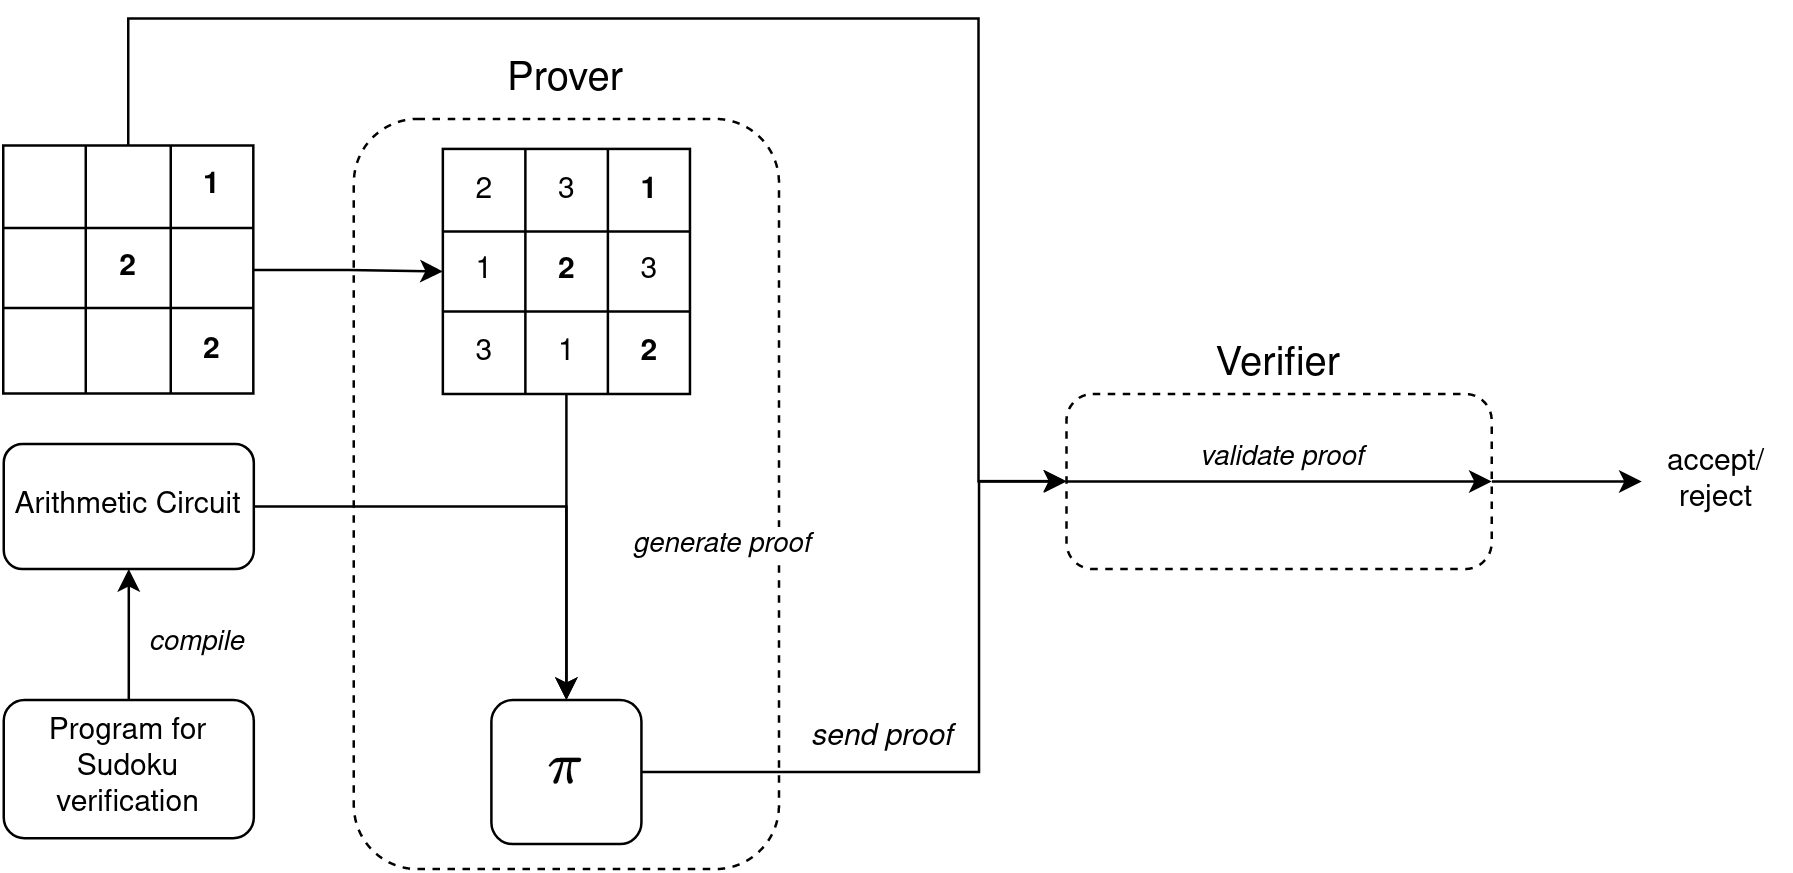
\includegraphics[width=1\linewidth]{figures/sudoku.drawio.png}
    \caption{Sudoku Example}
\end{figure}

% \begin{enumerate}
%     \item Encode circuit with secret and public parameters into polynomials
%     \item Generate a proof that this encoding was indeed done correctly
%     \item Verify that the proofs are valid
% \end{enumerate}



% %%%  ===========================================================================
% %%%  ===POLYNOMIALS=============================================================
% \section{Polynomials}
% % % \hl{reference how snarks work}
% Polynomials are mathematical objects studied for centuries, throughout this time we have figured out many nice and even some useful properties about them. One might ask what is so special about polynomials and it turns out a lot. They serve as a good tool for representing end encapsulating circuits. Let's show a simple observation:

% \begin{lemma}{Intersection of polynomials} \newline
%     Arbitrary two polynomials in form $a_0 + a_1x + a_2x^2 ... a_nx^n = 0; b_0 + b_1x + b_2x^2 ... b_m x^m = 0$ where both $n, m \leq d \in \mathbb{N}$ intersect in no more than $d$ points.
% \end{lemma}

% \begin{proof} \newline
%     To find the intersection points we need to solve equation $a_0 + a_1x + a_2x^2 ... a_nx^n = b_0 + b_1x + b_2x^2 ... b_m x^m$ which will produce yet another polynomial of degree $max(n,m) \leq d$. From the Fundamental Theorem of Algebra we know that a polynomial of degree $d$ cannot have more than $d$ roots.
% \end{proof}

% This a simple yet incredibly crucial observation for most of the proofs that will be carried out in this article. You can think about it as a tool for probabilistic polynomial identity testing, thanks to which we can effectively compare of two polynomials just by evaluating them at a uniformly random point. If polynomials are different we know they could intersect in at most $d$ points. The probability of randomly picking one of these points is $d$ divided by size of the domain. Depending on reasonably chosen parameters usually give negligible chances to guess the point correctly. Keep in mind the the domain size is given by $\lambda$. The observation can be generalized on multi-variate polynomials by Schwartz-Zippel lemma. % % \hl{include citation} To better understand how it works we will look at series of toy protocols, where we improve their faults in iterative manner. We will start with the most simple and crappy one:

% \begin{example} \textit{Polynomial Identity Check}

%     There is a verifier who knows some polynomial $p(x)$ and prover who wants to claim that he also knows coefficients of the polynomial $p(x)$. Say the polynomial has degree $d$ and the domain or evaluation range is $[1, 2^n]$. The prover could convince verifier as follows:
    
%     \begin{enumerate}
%         \item $V$ samples random point $r \in [1, 2^n]$
%         \item $V$ sends the point $r$ to $P$
%         \item $P$ sends back evaluation $p(r)$
%         \item $V$ locally computes $p(r)$ compares to what he got from $P$
%     \end{enumerate}    
% \end{example}

% With each $i$ iterations of this protocol the prover has probability of $(\frac{d}{2^{\lambda}})^i$ of guessing correctly. While this protocol is an interesting proof of concept, by itself it does not achieve much. Both of the parties know the same polynomial the only advantage is that the verifier does not compare coefficients of the polynomial but just one point. What might sound a bit more interesting is that a prover might be able to show that his polynomial $p(x)$ can be factored by $t(x)$ into $p(x) = t(x)h(x)$. 

% \begin{example} \textit{Polynomial Factor Check}

%     P wants to convince $V$ that he knows a polynomial $p(x)$ of degree $d$ with factor $t(x)$. In this protocol $P$ does not want to share $p(x)$ but wants to prove $p(x) = t(x)h(x)$, so naturally $V$ knows $t(x)$.
%     \begin{enumerate}
%         \item $V$ samples a random point $r$
%         \item $V$ sends the point $r$ to $P$
%         \item $P$ performs polynomial division $h(x) = \frac{p(x)}{t(x)}$ and sends evaluations of $p(r), h(r)$ to back to $V$
%         \item $V$ locally evaluates $t(r)$ and checks if $p(r) = t(r)h(r)$
%     \end{enumerate}
% \end{example}

% The protocol relies on the fact that $P$ is able to divide $p(x)$ if and only if $t(x)$ indeed is co-factor. Now we have a protocol in which the verifier is not revealed polynomial $p(x)$ and can relatively succinctly verify if it has some factor so all look good. Or does it? Well, no this protocol is terrible. The verifier gets to know some information about $p$ and that is the evaluation at $r$ and what is much worse the $P$ can cheat very easily in number of different ways:

% \begin{enumerate}
%     \item $P$ does not need to know the coefficients of $p$. He can quite easily calculate evaluation $t = t(r)$ and choose $h(r)$ such that $p(r) = t(r)h(r)$, without the verifier knowing.
%     \item $P$ nothing stops the prover from changing the $p$ on the fly. He know $r$ therefore, it is easy to construct any polynomial which has one shared polynomial with $t(r)h(r)$.
%     \item Nothing is constraining the $P$ to use polynomial of degree $d$. Prover can cheat by using polynomial $\widetilde{p}(x) = p(x)h'(x)$ with arbitrary $h'(x)$ that has bigger degree and also satisfies the factor check.
% \end{enumerate}

% The first two exploits possible because the prover knows $r$ and $t(r)$, thus he can temper with the protocol. Instead we would like to provide encrypted $r$ to the prover, so that he can use it as black box but does not know the real value. We will tackle this problem later by introducing homomorphic encryption, first we need a some understanding of elliptic curves.

\section{Elliptic curves}
The discussed elliptic curves will be over a finite field $\field$ where each for each point $(x, y) \in \field^2$. An elliptic curve is defined as $f(x,y): y^2 = x^3 + ax + b$ with parameters $a, b \in \field$. Points of the curve define a group $\mathbb{G}$ with a neutral element point at infinity $(0, 0)$ and $(x, -y)$ as the inverse element to $(x, y)$. In the following chapters, we will use multiplicative notation, and exponentiation will denote repeated application of the group operation.  We also denote $G$ a generator of the group $\mathbb{G}$. 

\hl{define DLP}

This group is especially interesting due to the hardness of the discrete logarithm problem (DLP), which is considered hard over sufficiently large $\field$. For this reason, $|\field|$ will be viewed as a security parameter of the $\plonk$ protocol. We will rely on the hardness of DLP on elliptic curves, which is standard in many modern cryptographic protocols.


\subsection{Elliptic Curve Arithmetic}
\label{sec:ec-arithmetic}

Given $G^a, G^b$, anyone can perform the operations listed below. However, it is very hard to extract $a, b$ due to DLP. That allows the prover to send some encoded values to the verifier, who will be able to perform arithmetic checks without discovering the original values.

\begin{table}[H]
    \centering
    \begin{tabular}{|l|l|l|l|}
    \hline
    \textbf{Operation}             & \multicolumn{1}{c|}{\textbf{Inputs}} & \textbf{Computation}            & \textbf{Result}    \\ \hline
    Addition              & $G^a, G^b$                  & $G^a \cdot G^b$        & $G^{a+b}$ \\ \hline
    Subtraction          & $G^a, G^b$                  & $G^a \cdot (G^b)^{-1}$ & $G^{a-b}$ \\ \hline
    Scalar multiplication & $G^a, \text{scalar } s$      & $(G^a)^s$              & $G^{as}$    \\ \hline
    Polynomial evaluation &
      \begin{tabular}[c]{@{}l@{}}$\{G, G^{a}, \ldots G^{a^n}\}$ \\ $f(x) = c_0 + c_1x + \ldots c_n x^n$\end{tabular} &
      $\prod_i (G^{a^i})^{c_i}$ &
      $G^{f(a)}$ \\ \hline
    \end{tabular}
\end{table}

The first two operations, addition and subtraction, follow from the definition of the group, and scalar multiplication is just a generalization of the exponentiation. For polynomial evaluation, take arbitrary polynomial $f(x) = c_0 + c_1 x + c_2 x^2 + c_3 x^3 + ... + x^n$ of degree bound $n$. The evaluation of $f(x)$ at some point $a$ can be written as 
$$G^{f(a)} = G^{c_0 + c_1 a + c_2 a^2  + ... + c_k  a^n} = (G^{a^0})^{c_0} \cdot (G^{a^1})^{c_1} \cdot (G^{a^2})^{c_2} \cdot \ldots (G^{a^k})^{c_n} = \prod_{i=0}^n (G^{a^i})^{c_i}$$



% \subsection{Homomorphic Encryption (inspiration how snarks work)}
% Remember the problem from example 2? Now we have all the tools to improve this protocol. We will use encryption function $E(r) = g^r$ where $g$ is a generator of elliptic curve group. Encrypting polynomial evaluated in $r$ with coefficients $c_i$ could be done as $E(r^i)^{c_i} = g^{r^i c_i}$. Evaluation of a polynomial will be denoted as: $E(p(r)) = g^{p(r)} =  (g^1)^{c_0} \cdot (g^{r^1})^{c_1} \cdot (g^{r^2})^{c_2} \cdot \ldots \cdot (g^{r^d})^{c_d}$. In order to make this more clear let's look at a specific example. Say we would like the prover to evaluate polynomial $p(x) = x^3 - 3x^2 +3x$ on the point $r$ without directly revealing $r$. Fist we need to encrypt values $E(r^3), E(r^2), E(r)$ which will be sent to prover. He can then reconstruct the polynomial as follows:

% $$E(r^3)^1 \cdot E(r^2)^{-3} \cdot E(r^3)^2$$
% $$g^{(r^3)^1} \cdot g^{(r^2)^{-3}} \cdot g^{(r^3)^2}$$
% $$g^{r^3 - 3r^2 + 2r}$$


% Given values $E(r^3), E(r^2), E(r)$ can now calculate evaluations $g^{p(r)}, g^{h(r)}$ in the encrypted space. The verifier will also validate the result in encrypted space by checking is $g^{p(r)} = g^{h(r)}g^{t(r)}$. These conditions make life of a dishonest prover much harder, because now he does not know much about the secretly sampled value $r$. % % \hl{more rigorou explanation for why it is harder}
% We have now greatly limited the possibilities of cheating the protocol is still not sound. 

% Remember that there was also a third point, which said that there is nothing constraining the prover to using polynomial of a different degree. Although we have restricted the prover in selection of powers of $r$ we have not restricted him to using them. That is why the verifier need a prove that only the supplied encryption were used to calculate $g^{p(r)}, g^{t(r)}$ and nothing else.


\subsection{Elliptic curve pairing}
\hl{add explanation of groups}

Pairing $e$ is in essence deterministic mapping to another group $e: \mathbb{G}_1 \times \mathbb{G}_2 \rightarrow \mathbb{G}_t$. To be more specific, it is a bilinear mapping that takes two encrypted elements from the source group and combines them into an element of the target group. Since this is a complex topic, we will treat the pairing as a black box; for a more detailed explanation, we refer the reader to \cite{ec-pairings}. For the purposes of this work, it will be sufficient to know that curve pairings have the following properties $\forall a, b \in \field$:
$$e(G_1^a, G_2^b) = e(G_1^b, G_2^a) = e(G_1^{ab}, G_2^1) = e(G_1^1, G_2^{ab}) = e(G_1^1, G_2^a)^b = e(G_1^1, G_2^1)^{ab}$$

In \Cref{sec:ec-arithmetic}, there is no way to calculate $G^{a \times b}$ from $G^a, G^b$. We will use curve pairings to "emulate" this operation $e(G_1^a, G_2^b) = G_t^{ab}$. Note that the operation cannot be performed more than once because the result is in a different target group. Thus, we will be allowed to use this operation in the $\plonk$ protocol only a single time. Not all elliptic curves are pairing-friendly, and this property is rather rare.

\subsection{Multi-scalar Multiplication}
Polynomial evaluation can be performed via multiscalar multiplication (MSM), where elements $\{G, G^a, G^{a^2}, \ldots, G^{a^n}\}$ are pairwise multiplied by scalars $\{c_0, c_1, c_2, \ldots, c_n\}$ and eventually summed. In the group $\mathbb{G}$, the scalar multiplication $(G^{a^i})^{c_i}$ is defined as $c_i$ times repeated group operation $G^{a^i} \cdot G^{a^i} \ldots G^{a^i}$. When dealing with fields in order hundreds of bits, this becomes expensive, and this operation is a major bottleneck of $\plonk$ and many SNARK protocols.

To make this operation faster, it is possible to calculate the elements using the \textit{square and multiply} version, which can be described as:

\begin{equation*}
    (G^{a_i})^n = 
    \begin{cases}
        ((G^{a_i})^2)^{n/2} & 2 \mid n \\
        G^{a_i}((G^{a_i})^2)^{(n-1)/2} & 2 \nmid n 
    \end{cases}
\end{equation*}

The naive way needs to perform $n$ group operations to calculate $(G^a_i)^n$ while \textit{square and multiply} achieves the same result in $\bigO{\log_2{n}}$. The resulting complexity of MSM is $\bigO{n \times  \log_2{\max_i{c_i}} }$.
% $n-1 + \lceil \log_2{c_0} \rceil, \lceil \log_2{c_1} \rceil, \ldots \lceil \log_2{c_n} \rceil \rightarrow \bigO{n \times \lceil \log_2{\max_i{c_i}} \rceil}$. 

\hl{make sure the assumption that the field is much bigger than the degree of the polynomials}
\hl{make simpler delete lambda}
A more efficient way is to use Pipenger's algorithm \cite{Pippengers} with complexity $\bigO{\lambda\frac{n}{\log_2(n)}}$ where $\lambda$ is dependent on the algorithm parameters. There are possible improvements to this algorithm in the form of precomputation and parallelism. In practice, there is also an effort to create a hardware-accelerated version of MSM, described in PipeMSM \cite{pipeMSM}.
% ==============================================================================
% ===POLYNOMIALS================================================================
% ==============================================================================
\section{Polynomial toolkit}

\subsection{Comparing polynomials}
\label{comparing-poly}

Effective comparison of polynomials is one of the building blocks of $\plonk$. We can test if two polynomials are equal just by comparing them at a uniformly random point. 
\begin{theorem}
\label{theorem:poly-intersection}
    Arbitrary two non-identical polynomials $a_0 + a_1x + a_2x^2 ... a_nx^n; b_0 + b_1x + b_2x^2 ... b_m x^m$, where both $n, m \leq d \in \mathbb{N}$ intersect in no more than $d$ points.
\end{theorem}{Intersection of polynomials}

\begin{proof}
    An intersection point $\gamma$ such that $$a_0 + a_1 \gamma + a_2 \gamma^2 \ldots a_n \gamma^n = b_0 + b_1 \gamma + b_2 \gamma^2 \ldots b_m \gamma^m,$$ 
    is a root of the following polynomial of degree $max(n,m) \leq d$
    $$a_0-b_0 + (a_1-b_1)x + (a_2-b_2)x^2 \ldots (a_n - b_n)x^n = 0.$$
    From the Fundamental Theorem of Algebra, we know that a polynomial of degree $d$ cannot have more than $d$ roots.
\end{proof}

If two polynomials are identical, then $\forall x: p(x) = q(x)$, so determining identity based on evaluation at a random point is correct. Two polynomials with different coefficients can be equal at intersection points, so this approach has a soundness error rate. Based on \Cref{theorem:poly-intersection}, two non-identical polynomials might intersect in almost $d$ points, so the probability of randomly selecting one of the intersection points is $\frac{d}{\text{domain size}} = \frac{d}{|\field|}$. This probability is considered negligible. For example, the commonly used elliptic curve $BLS12-381$ has order $\approx 2^{381}$. The failure rate is small enough for most practical purposes, so we can compare two polynomials just by a single evaluation.

\hl{what is usually d give an example}

A multivariate version of the previous observation could be proved by the Schwartz-Zippel lemma \cite{schwartz-lemma}.

\begin{lemma}
\label{sz lemma}
    For domain $D \in \field$ and a polynomial $f(x_1, x_2, \ldots x_n) \in \field[x_1, \ldots, x_n]$ with degree bound $d$ and  independently uniformly at random selected $(r_1, r_2 \ldots r_n) \in D^n$ it holds:
    $$\prob{f(r_1, r_2 \ldots r_n) = 0} \leq \frac{d}{|D|}.$$
\end{lemma}


\subsection{Evaluation domain}
To create the evaluation domain, we use the primitive $n$-th root of unity $\omega \in \field$ for which it holds that $\omega^n = 1$ and $\forall 1 \leq i < n: \omega^i \neq 1$. The evaluation domain $H$ will be constructed as $$H = \{1, \omega, \omega^2 \ldots \omega^{n-1}\}.$$

This domain will be especially useful because it allows for a sparse representation of certain polynomials. This results in numerous benefits, such as faster polynomial evaluation.

\begin{definition}[Vanishing polynomial]
    Denote $Z_H(x)$ the vanishing polynomial for the domain $H$ such that $\forall x \in H: Z_H(x) = 0$ and deg $deg(Z_H) = |H|$.
\end{definition}

Since the vanishing polynomial has roots as the elements of $H$, it could be written as: $$Z_H(x) = (x-1)(x-\omega)(x-\omega^2) \ldots (x-\omega^{n-1}).$$
However, the domain $H$ also allows for a sparse representation of this polynomial $Z_H(x) = x^n-1$. To observe that this holds, we verify $$\forall x \in H: x^n-1 = (\omega^i)^n - 1 = (\omega^n)^i - 1 = 1^i - 1 = 0.$$



    
\subsection{Lagrange basis}
In the $\plonk$ paper, interpolation is performed using the Lagrange basis.

\begin{definition}[Lagrange basis]
    We denote by $L_i$ the $i$th polynomial of the Lagrange basis over $H$ as:
    $$
    L_i(x) = 
        \begin{cases} 
            1 & x = \omega^i \\
            0 & \text{otherwise}
       \end{cases}
    $$
\end{definition}

Given a vector $v = [v_0, v_1, \ldots ,v_{n-1}]$, we interpolate it over the domain $H$ via the polynomial:$$v(x) = \sum_{i=0}^{n-1}v_iL_i(x).$$

The Lagrange basis can be expressed as:  $$L_i(x) = \prod_{k \in H, k \neq \omega^i} \frac{x-k}{\omega^i-k}.$$

The properties of this polynomial are easy to observe. When $x \in H \setminus \{ \omega^i \}$ is plugged into $L_i(x)$, then there is exactly one fraction for which $k = x$, which makes the product 0. If $x = \omega^i$, the consequence is even more trivial because all of the fractions would result in $\frac{\omega^i-k}{\omega^i-k} = 1$, and since $k \neq \omega^i$, $L_i(\omega^i)$ results in 1.

Due to the choice of the evaluation domain, the Lagrange basis also has a sparse representation as presented in \cite{BarycentricLagrange}. 
$$L_i(x) = \frac{b_iZ_H(x)}{x - \omega^i},$$
$$b_i = \prod_{k \in H, k \neq \omega^i} \frac{1}{x_i - x_k}.$$

Notice that each $b_i$ depends only on the elements of the domain $H$. So, all of the values $b_i$ could be precomputed.

%%%  ===========================================================================
%%%  ===COMMITMENT SCHEME=======================================================
\section{Polynomial Commitment Scheme}
A commitment scheme is a cryptographic primitive that makes it possible to commit to a piece of information, ensuring that it remains unchanged throughout the process of verification. One motivation for this mechanism is to prevent the prover from generating proofs depending on the verifier's queries. In the context of $\plonk$, we will rely on the polynomial commitment scheme, where the prover knows the coefficients of some polynomial $f(x)$ and wants to prove evaluation of $f$ at a point given by the verifier. 

A standard polynomial commitment scheme has the following procedures:
\begin{enumerate}
    \item $\mathsf{Setup(\secparam)} \rightarrow \publicparameter$: generate public parameters.
    \item $\mathsf{Commit}(f, \publicparameter) \rightarrow c$: calculate commitment $c$ which binds $\prover$ to the polynomial $f(x)$.
    \item $\mathsf{Open}(z, \publicparameter) \rightarrow (v, \pi):$ given the challenge $z$, $\prover$ returns a pair $(v, \pi)$, where $\pi$ is the proof that $v = f(z)$.
    \item $\mathsf{Verify}(\publicparameter, c, z, v, \pi) \rightarrow \mathsf{accept/reject}$: $\verifier$ checks validity of the claim $f(z) = v$.
\end{enumerate}

\procedureblock{Polynomial Commitment Scheme}{    
    \textbf{Prover } \prover \>\> \textbf{Verifier } \verifier \pclb
    \pcintertext[dotted]{Scheme Setup}
    \mathsf{Commit} \> \sendmessageright*[6cm]{c} \> \\
    \> \sendmessageleft*[6cm]{z} \> z \gets \field \\
    \mathsf{Open} \> \sendmessageright*[6cm]{(v, \pi)} \> \\
    \> \> \mathsf{Verify} \\
    % \>\> \pcreturn accept/reject
}

\hl{odkaz an diagram}
We will require that the commitment is \textit{binding} and \textit{hiding}. Loosely speaking, binding means that the commitment binds the prover to a specific polynomial. Hiding property suggests that the prover does not discover the coefficients of the polynomial $f(x)$. We will define it more formally.

\begin{definition}{Evaluation binding}
    guarantees that any efficient prover is unable to generate a convincing $\pi$ for $v = f(z)$ and $\pi'$ for $v' = f(z)$.
\end{definition}

Computational hiding property says that for polynomial $f(x)$ and its commitment $c$ and any efficient $\adv$, the polynomial $f(x)$ is computationally indistinguishable from a randomly chosen polynomial. We will achieve the hiding of the scheme in \Cref{sec:blinding} with a stronger property — zero-knowledge.


The next notion we formalize ensures that if the verifier accepts the proof, the prover needs to have knowledge of the committed polynomial.

\begin{definition}{Extractable scheme}
    guarantees that for all efficient provers $\prover$ that takes as input public parameters, degree bound $d$ and outputs commitment $c$ $\exists$ efficient extractor algorithm $\extractor$ that has the same input as $\prover$ and produces polynomial $f(x)$ of bound $d$ explaining all of $\prover$ answers to evaluation queries.
    % such that evaluation queries on $f(x)$ correspond to answers of $\adv$ to these queries.
\end{definition}

The extractability of a polynomial commitment is stronger than binding as it was with soundness and knowledge soundness in \Cref{prelim}. It guarantees that for any efficient prover capable of passing all of the checks, the prover must actually “know” a
polynomial p of the claimed degree that explains its answers to all evaluation queries.

% Extractability suggests that the prover needs to have knowledge of $f(x)$ and it can be extracted from him. That follows from the fact that $E$ is efficient and therefore an efficient $\mathcal{A}$ can afford to run it. Since $E$ does not know anything more than $\mathcal{A}$ and can produce $f(x)$ that can use $E$ to get knowledge of $q$, which passes all queries.


\subsection{KZG Polynomial commitment scheme}
The KZG polynomial commitment scheme, based on the pairing (elliptic curve) group, was introduced in \cite{KZG}. It has constant proof size and requires a trusted setup. There are other ways to design polynomial commitment schemes, such as \cite{fri} based on hash functions. We will explain KZG since it is used in the $\plonk$ protocol. This section is heavily inspired by the work of Justin Thaler in \textit{Proofs, Arguments, and Zero-Knowledge} \cite{ProofArgsAndZk}. We will try to explain an imperfect, non-extractable KZG polynomial commitment and provide ideas of the proofs, but for the proper security analysis of KZG, we refer the reader to the Section 15.2 \textit{Proofs, Arguments, and Zero-Knowledge} \cite{ProofArgsAndZk}.

The public parameters $\publicparameter$ of the KZG is the \textit{structured reference string} (SRS) consisting of evaluations $\{G, G^{\tau}, G^{\tau^2}, ..., G^{\tau^{d-1}}, G^{\tau^{d}}\}$, where $d$ is degree bound of committed polynomial and $\tau$ is uniformly randomly chosen $\tau \gets \field$. The setup of the protocol needs to be trusted because if the prover discovers the value $\tau$, it will allow him to forge proofs and, thus, prove any evaluation. So naturally, the setup either needs to be computed by the verifier or via a secure multiparty computation. Below, we list all public information for the KZG scheme:

\begin{enumerate}
    \item $\mathbb{G}_1, \mathbb{G}_2$ are pairing friendly groups both under the field  $\field$ for $p$ prime
    \item $G_1, G_2$ are generators of $\mathbb{G}_1, \mathbb{G}_2$
    \item $e$: is a symmetric bilinear map meaning in $\mathbb{G}_1 \times \mathbb{G}_2 \rightarrow \mathbb{G}'$ the groups $\mathbb{G}_1$ and $\mathbb{G}_2$ are equal.
    \item $d$ is the upper bound on the polynomial degree
    \item SRS evaluations $\{G, G^{\tau}, ... ,G^{\tau^d}\}$
\end{enumerate}

Before we proceed to describe the procedures, we need to introduce an observation that allows us to effectively transform equality checks into divisibility checks. The polynomial we get from the division will be used as the proof of evaluation.  

\begin{lemma}
    \label{evaluation-proof}
    For any degree $d$ univariate polynomial $f \in \mathbb{F}_p[x]$ the assertion $f(z) = v$ is equivalent to checking if there exists a polynomial $w(x) \in \field[x]$ of degree at most $d - 1$ such that: $w(x) = \frac{f(x)-v}{x-z}$.
\end{lemma}

\begin{proof}
    In the forward directions, we have a polynomial $f(x)$, and we know that $f(z) = v$. We can construct $\widetilde{f}(x) = f(x) - v$ which is 0 at $z$. If $\widetilde{f}(z) = 0$ then $z$ is the root of $\widetilde{f}(x)$ so $\widetilde{f}(x)$ could be also written as $\widetilde{f}(x) = (x-z)w(x)$. Now we just reorder the expression:
    $$\widetilde{f}(x) = (x-z)w(x),$$
    $$w(x) = \frac{\widetilde{f}(x) }{x-z},$$
    $$w(x) = \frac{f(x) - v}{x-z}.$$

    In the opposite direction, we have polynomial $w(x) = \frac{f(x) - v}{x-z}$ and want to show that $f(z) = v$. If we have $w(x)$ it means that $\widetilde{f}(x)$ is divisible by $x-z$, so $z$ is the root of $\widetilde{f}(x)$ which implies $f(z) = v$. 
    % To prove $q(z) = v$ implies existence of $w(x)$ we simply plug $z$ into $q(x)-v = w(x)(x-z)$ which results into $0 = w(x)0$. This is satisfied for an arbitrate polynomial. The other way around, we have $w(x) = \frac{q(x) -v}{x-z}$ and want to show that $q(z) = v$. By looking just at $q(x)-v = w(x)(x-z)$, we could notice that if we shift the polynomial $q(x)$ down by $v$, then it has a root at point $z$. For a polynomial $r(x) = q(x) - v$ the evaluation of $r(z) = 0$. In each evaluation, the values of $r$ and $q$ differ by $v$. So if we know that $r(z) = 0$, then it must follow that $q(z) = v$, which is what we wanted to achieve.
\end{proof}

\subsubsection{Commitment}
To commit to $f(x)$ over $\mathbb{F}_p$ $\prover$ sends $c \in \mathbb{G}_1$ which he claims is $f(\tau)$ encoded as elliptic curve point $G_1^{f(\tau)}$. We use the notation $G_1^{f(\tau)} = [f]_1$. However, above, we have said that the prover should not be able to discover $\tau$ under any circumstance, so how does he compute $f(\tau)$? The trick is that he does not have to know $\tau$ to compute the commitment. Recall from \Cref{sec:ec-arithmetic} that function evaluation $f(\tau)$ only requires to know the coefficients of $f(x)$ and $\{G, G^{\tau} \ldots G^{\tau^d}\}$ which is provided as the SRS public key. This way, the prover is able to compute $G^{f(\tau)}$ without knowing $\tau$.

\subsubsection{Opening}
To open for challenge $z$, the prover computes the opening proof polynomial:
$$w(x) = \frac{f(x)-v}{x-z}.$$

By \Cref{evaluation-proof}, we know that proving the existence of $w(x)$ is equivalent to $f(z) = v$. Assuming $\prover$ knows $f(x)$, he is able to calculate $G^{w(\tau)}  = [w_1]$ and evaluate $f(z) = v$. Finally, the prover sends $(v, [w]_1)$ to the verifier. 

\subsubsection{Verification}
The verifier knows $c, v, g^{w(\omega)}$ provided by the prover, $z$ generated by himself and the public SRS. The only check that needs to be done by $\verifier$ is:
$$e(cG_1^{-v}, G_2) \stackrel{?}{=} e(G_1^{w(\omega)}, G_2^{\omega} G_2^{-z}).$$
Note that from the whole SRS, only $(G_1, G_2, G_2^\omega)$ are needed for the evaluation, which is why in many works, SRS is referred to as a prover key and $(g, g^\omega)$ as a verification key. 

\hl{kzg-correctnes make sure this ref in not broken}
To prove correctness: $$e(G_1^{w(\omega)}, G_2^{\omega} G_2^{-z}) = e(G_1^{\frac{f(\omega) -v}{\omega -z}}, G_2^{\omega -z})$$ 
$$= e(G_1, G_2)^{f(\omega) -v} = e(G_1^{f(\omega)-v} G_1, G_2) = e(c G_1^{-v}, G_2).$$

The last step of this expansion is true if and only if $c = g^{f(\omega)}$. For an honest prover who knows $f(x)$, the verification procedure would accept with probability 1, which shows the correctness of the protocol. The complete scheme is summarized in the next figure.

\hl{again cref for cryptocode}

\pseudocodeblock[head=KZG polynomial commitment scheme]{
    \text{Prover } \prover \< \< \text{Verifer } \verifier \\
    \< \< \\[-0.8 \baselineskip] \\
    \mathsf{Commit} \< \sendmessageright*{\relax[f]_1} \> \\
    \< \sendmessageleft*{z} \< z \gets \field \\
    f(z) = v \< \< \\
    w(x) = (f(x) - v) / (x-z) \< \< \\
    \mathsf{Open} \< \sendmessageright*{([w]_1, v)} \< \\
    \< \< \mathsf{Verify} \\
    \< \< e(cG_1^{-v}, G_2) \stackrel{?}{=} e(G_1^{w(\omega)}, G_2^{\omega} G_2^{-z})
}

Why does this commitment scheme need to use pairing groups? Notice that the verifier is not able to calculate "multiplication in exponent" $G^{w(\tau) \times (\omega - z)}$. As suggested in the \Cref{sec:ec-arithmetic}, it is possible to solve this by using pairing.

% Why all of the hassle with curve pairing, what is it used for? A mindful reader might have noticed that otherwise the verifier would not be able to perform the check. In detail the left side $g^{q(w) - v} = g^{q(w)} g^{-v}$ is easily computable, since $\verifier$ gets $g^{q(w)}$ can find exponentiate $g^v$ and then take the negative. Problem is with the right side where $\verifier$ has $g^{w(\omega)}, g^\omega, z$, thus can compute $g^{\omega - z}$, however $g^{w(\omega) (\omega - z)} = g^{w(\omega)^{(\omega - z)}}$. Remember that the value of $\omega$ is secret and should be destroyed immediately after setup, which means $\verifier$ has knowledge of $g^\omega$ but no $\omega$. This means he cannot calculate $(\omega - z)$ and thus is is not possible to compute $w(\omega) (\omega - z)$ in the exponent. Luckily this operation can be performed via curve pairing thanks to the property $e(g^a, g^b) = e(g, g)^{ab}$.

\subsection{KZG analysis}
\label{chap:kzg}

\subsubsection{Hiding}
The verifier gets the commitment $c = G_1^{f(\tau)}$, which is one evaluation of the commitment polynomial, and the real value is infeasible to extract due to DLP. The prove also sends tuple $(v, G^{w(\tau)})$ where $w(\tau)$ cannot be obtained from the proof of opening also because of DLP. However, the evaluation $v = f(z)$ is sent in plaintext form. This means that the verifier discovers some information about the committed $f(x)$. The KZG commitment scheme could be potentially computationally hiding if executed just once. If we do not limit the number of openings, the verifier might eventually get $d$ evaluation of the committed polynomial $f(x)$, which would allow him to reconstruct the polynomial by interpolation.

We cannot rely on the KZG polynomial commitment scheme to sufficiently hide the committed polynomial $f(x)$. Therefore, we will use blinding in \Cref{sec:blinding} to achieve zero-knowledge for specific cases.

% Then, as a part of verification, $\prover$ sends $G^{w(\tau)}$, where $w(\tau)$ is likewise not possible to extract. After executing KZG commitment scheme $\verifier$ has two encrypted evaluations which reveal no information thanks to DLP and one plain text evaluation to the committed polynomial. To properly establish a hiding property, the polynomial $q$ has to be indistinguishable from a randomly chosen polynomial of the same degree. % % \hl{How to construct hiding game}

\subsubsection{Binding}
Binding property is a little harder to establish. First, we introduce the cryptographic assumption SDH.

\begin{definition}{Strong Diffie Hellman Assumption}
    SDH assumes that, given $\publicparameter$, $\prover$ has no efficient way of computing a pair $(z, G^{\frac{1}{\tau - z}})$. 
\end{definition}

This assumption is stronger than DLP itself. We will show that this assumption needs to hold. Otherwise, $\prover$ would be able to give two different openings for the same challenge, which breaks the evaluation binding property.

\begin{lemma}
    Assuming the Strong Diffie-Hellman assumption holds, $\prover$ can provide only one valid opening $v$ for any challenge $z$ in the KZG scheme. 
\end{lemma}

\begin{proof}
    For a contradiction, we can say that $\prover$ is able to prove two different openings $v \neq v'$ of committed $f(x)$ at a challenge $z$. This would require calculating two different proofs of opening $w(\omega), w'(\omega)$:
    \[
    \begin{array}{cc}
         w(\tau) = \frac{f(\tau) - v}{\tau - z} & w'(\tau) = \frac{f(\tau) - v'}{\tau - z} \\
    \end{array}
    \]
    
    $$w(\tau) - w'(\tau) = \frac{v' - v}{\tau - z}$$
    $$\frac{1}{\tau - z} = \frac{w(\tau) - w'(\tau)}{v' - v}$$
    $$G^{\frac{1}{\tau - z}} = \frac{1}{{v' - v}}G^{w(\tau) - w'(\tau)}$$

    We get a contradiction because we can use such a prover to break the SDH assumption.
\end{proof}

\subsubsection{Extractable scheme}
To make KZG extractable, we need to modify it. The SRS will be twice as long containing pairs $$\{(G_1, G_1^{\psi}), (G_1^{\tau}, G_1^{\tau \psi}), (G_1^{\tau^2}, G_1^{\tau^2 \psi}) \ldots (G_1^{\tau^d}, G_1^{\tau^d \psi})\} \text{ for } \psi \gets \field, \tau \gets \field$$

\begin{definition}[Power Knowledge of Exponent assumption]
    For any efficient $\mathcal{A}$ given access to SRS, whenever $\adv$ outputs group elements $a, b \in \mathbb{G}$ such that $a = b^{\psi}$ then  $\adv$ needs to know the coefficients that explain $a = \prod_{i=0}^d = G^{c_i \tau^i}$ and $b = \prod_{i=0}^d = G^{c_i \tau^i \psi^i}$.
\end{definition}

Now, the commitment will be a pair $c = (G_1^{f(\tau)}, G_1^{f(\tau \psi)})$. The calculation of the witness polynomial remains the same, and the verifier now needs to perform two checks:

\begin{equation}
    \label{extractability1}
    e(G_1^{f(\tau)} G_1^{-v}, G_2) \stackrel{?}{=} e(G_1^{w(\tau)}, G_2^{\tau} G_2^{-z})
\end{equation}

\begin{equation}
    \label{extractability2}
    e(G_1^{f(\tau)}, G_2^\psi) \stackrel{?}{=} e(G_1^{f(\tau \psi)}, G_2)
\end{equation}

The correctness of \Cref{extractability1} holds based on the correctness of the previous KZG explanation and the correctness of \Cref{extractability2} holds because of:

\[
\begin{array}{cc}
     G_1^{f(\tau)} & G_1^{f(\tau \psi)} \\
     \prod_i (G_1^{\tau^i})^{c_i} & \prod_i (G_1^{\tau^i \psi})^{c_i} \\
     \prod_i (G_1^{\tau^i})^{c_i} & \prod_i (G_1^{\tau^i})^{c_i \psi} \\
     \relax[f]_1 & [f]_1^\psi \\
\end{array}
\]

Very intuitively, this variant of the KZG polynomial commitments scheme remains binding because the modification scheme only extends to one more verification check, but the first one already binds the commitment to a specific polynomial. To prove the extractability of the scheme, we rely on the second verification check, which simplifies to $g^{q(\psi \omega)} = g^{\omega} g^{\psi}$. From the PKoE, it needs to follow that $\adv$ has knowledge of the coefficients and, therefore, knows the polynomial $f(x)$. More details about the proof can be found in Proofs, Arguments, and Zero-Knowledge \cite{ProofArgsAndZk}.


% \subsubsection{Time analysis}
% To analyze the complexity of the final protocol we want to know how to KZG polynomial commitment scheme performs. The big advantage is that the commitment is constant in size because it is always just one group element. On the other hand $SRS$ is a lot bigger with $d$ elements from $\mathbb{G}_1$ and one element from $\mathbb{G}_2$. This requires significant computation but is done only once. Moreover, the prover requires only 2 elements from $SRS$. 

% In the prover (committer) algorithm, there needs to be calculated commitment $C$ and witness $W$ and each requires a single MSM. Evaluation of $v$ can be done in constant time. Moreover to generate the witness the prover needs to do a polynomial division which is $O(n^2)$ in the common approach.

% The verifier needs to compute $g^{-v}$ and also $g^z$ and two pairings. 1 $\mathbb{G}_1$ scalar multiplication, 1 $\mathbb{G}_2$ scalar multiplication and 2 pairings.

\subsubsection{Blinding}
\label{sec:blinding}
We have discussed the KZG commitment scheme, which is not zero-knowledge. Openings clearly reveal some information about the committed polynomial. To make $\plonk$ zero-knowledge, we will randomize the committed polynomial. The $\plonk$ protocol  suggests to blind a polynomial $f(x)$ as follows: $$\widetilde{f}(x) = Z_H(x) \times \text{some expression} + f(x)$$

Notice that the polynomials $f(x), \widetilde{f}(x)$ agree on all points of domain $H$ because $Z_H$ evaluates to zero over $H$. The checks of the $\plonk$ protocol only verify properties on the evaluation domain $H$, which is why it does not matter that $f(x), \widetilde{f}(x)$ might not match outside of $H$.

Consider that some polynomial $f(x)$ should be opened at challenge points $(z_1 \ldots z_{k})$ randomly chosen by the verifier. We alter the committed polynomial with uniformly randomly and independently chosen blinding scalars $(b_1, b_2, \ldots, b_{k+1}) \gets \field$ as $$\widetilde{f}(x) = (b_1 + b_2x + b_3x^2 ... + b_{k+1}x^{k})Z_H(x) + f(x)$$

Notice that the degree of the blinding polynomial depends on $k$, the number of openings. Does the opening of $\widetilde{f}(x)$ reveal any information about $f(x)$? Well, of course, it does, because for $\forall x \in H: f(x) = \widetilde{f}(x)$. However, $|H|$ is orders of magnitude smaller than $|\field|$, and the probability of randomly choosing an element of $H$ is considered to be negligible. Let's examine the case when $x \neq H$.

\begin{definition}[$k$-blinded polynomial]
    A polynomial $\widetilde{f}(x)$ is constructed as
    $$\widetilde{f}(x) = b_k(x)Z_H(x) + f(x)$$
    where $b_k(x) = b_1 + b_2x + b_3x^2 \ldots + b_{k+1}x^{k} + b_{k+2}x^{k+1}$ is a blinding polynomial with coefficients chosen independently and uniformly randomly and $Z_H(x)$ is polynomial vanishing on domain $H$.
\end{definition}


% \begin{definition}
%     A protocol $(\ldots)$ has $k$-wise zero-knowledge if there exists a probabilistic poly-time simulator $S$ such that for all interactive non-uniform polynomial time adversaries $\adv$

%     \[
%     \operatorname{Pr}
%     \left[
%     \begin{array}{c}
%         srs \gets \mathsf{Gen}(d) \\
%         c \gets \mathsf{Commit}(srs, q) \\
%         (z_1, z_2, ..., z_k) \gets \adv \\
%         (y, v_1, v_2, ..., v_k) \gets \mathsf{Eval}(srs, q, z)
%     \end{array}
%     :
%     \adv(c, (z_1, z_2, ..., z_k), (v_1, v_2, ..., v_k), g^{w(\tau)}) = 1
%     \right]
%     \]
    
%     \[
%     =\operatorname{Pr}
%     \left[
%     \begin{array}{c}
%         srs \gets \mathsf{Gen}(d) \\
%         (c, (v_1, v_2, ..., v_k), y) \gets \mathsf{Sim}(srs, (z_1, z_2, ..., z_k)) \\ 
%     \end{array}
%     :
%     \adv(c, (z_1, z_2, ..., z_k), (v_1, v_2, ..., v_k), y) = 1
%     \right]
%     \]
    
% \end{definition}

% \hl{use the definition and just specify L as language }


% \begin{definition}{Honest verifier zero-knowledge (HVZK)}
%     An interactive proof system $\langle \prover, \verifier \rangle$ honest verifier zero-knowledge if there exists
%     a probabilistic polynomial time simulator $\mathsf{Sim}$ with access to the verifier such that:
%     $$\forall x \in \mathcal{L}: \mathsf{Sim}(x) \approx View_{V}(\langle \prover, \verifier \rangle(x))$$
    
%     Where $\mathsf{Sim}(x)$ and $View_{V}(\langle \prover, \verifier \rangle(x))$ are distributions with the randomness of $\verifier$, and $View_{\verifier}(\langle \prover, \verifier \rangle(x))$ all entries in the honest transcript.
% \end{definition}

We would like to show that proving at most $k$ polynomial evaluation of $k$-blinded polynomial using the KZG polynomial commitment scheme is honest verifier zero-knowledge as captured by \Cref{hvzk}. In the context of KZG, the transcript of $k$ opening proofs for committed polynomial $f(x)$ with an evaluation proof polynomials $w_1(x), \ldots w_k(x)$ will be denoted as $$(C = G_1^{f(\tau)}, \bar{z} = \{z_1, \ldots, z_k\}, \bar{v} = \{v_1, \ldots, v_k\}, \bar{W} = \{G_1^{w_1(\tau)}), \ldots, G_1^{w_k(\tau)})\} .$$ 

\begin{definition}[Honest Transcript]
    The honest transcript is $(C, \bar{z}, \bar{v}, \bar{W})$ generated from the interaction of a non-malicious prover and verifier where the prover knows the committed polynomial and the verifier accepts the provided openings. 
\end{definition}

To prove that blinding guarantees honest verifier zero-knowledge, we need to show the construction of a simulator that produces an indistinguishable transcript from an honest transcript. First, we describe a few useful observations. We will again define the zero-knowledge property specific to this case.

\begin{definition}[Honest Verifier Zero-Knowledge for KZG analysis]
    The polynomial commitment scheme $(\mathsf{Setup}, \mathsf{Commit}, \mathsf{Open}, \mathsf{Verify})$ is honest verifier zero-knowledge (HVZK) if there is an efficient simulator $\simulator$ for any combination of a function $f(x)$ such that the distribution:
    $$(C, \bar{z}, \bar{v}, \bar{W}): 
    \begin{array}{c}
        \publicparameter \gets \mathsf{Setup}(\secparam) \\
        C \gets \mathsf{Commit}(f, \publicparameter) \\
        (v, W) \gets \mathsf{Open}(z, \publicparameter)
    \end{array}
    $$
    % \publicparameter \gets \mathsf{Setup}(\secparam), c \gets \mathsf{Open}(f, \publicinput), (v, W) \gets \mathsf{Open}(\publicparameter, z)$$
    is computationally indistinguishable from
    $$(C, \bar{z}, \bar{v}, \bar{W}) \gets \simulator(\publicparameter)$$
\end{definition}

\begin{lemma}
\label{lemma:addition-randomness}
    $\forall x \in \field, a \gets \field$ where $a$ is non-zero element the function $f_a(x) = x + a$ defines a random permutation of elements of $\field$.
\end{lemma}

\begin{proof}
    To show that $f_a(X)$ is a permutation we want:
    $$\{0, 1, 2, \ldots, p\} = \{0+a, 1+a, 2+a, \ldots, p+a\}$$
    
    Assume there exist $x_1, x_2 \in \field, x_1 \neq x_2: f_a(x_1) = f_a(x_2)$. Then $x_1 + a = x_2 + a \implies x_1 = x_2$, which is a contradiction. Therefore we can say that $f_a(x)$ is injective. Since adding two field elements of the field results in another element of the same field the $f_a$ needs to be subjective. From there it follows that $f_a(x)$ is a permutation function determined by the randomness of $a$.
\end{proof}


\begin{lemma}
\label{lemma:multiplication-randomness}
    For the generator $G_1$ of a group $\mathbb{G}_1$ and a random element $a \gets \mathcal{U}_{\field}$ the group element $G_1^a$ is a uniformly random element of the group generated by $G_1$.
\end{lemma}

\begin{proof}
    Since $a$ is chosen uniformly at random from the field, and $G_1^a$ maps each element in the field to a unique element in the group $\mathbb{G}_1$, the image of this function  must also be uniformly distributed across the group.
\end{proof}

\begin{lemma}
\label{lemma:kwise-eval}
    Given prime $p$ and a polynomial over a finite field $\field$ of degree bound $k$ with independently randomly chosen coefficients we can evaluate it at $k$ independently randomly chosen values and get $k$ independent uniformly random field elements.
\end{lemma}

The above lemma is used in constructing $k$-wise independent hash functions first described by \cite{WEGMAN-kwise-hash}, therefore we do not include the proof. The intuition is that a polynomial of degree $k$ is uniquely defined by $k+1$ points, which can be interpolated. When provided only $k$ points, each polynomial of degree $k$ is equally probable. Since each of the polynomials has a uniform probability, we get that any $k$-tuple of distinct arguments is equally likely to be mapped to any $k$-tuple of evaluations.

\begin{lemma}
\label{lemma:blinded-kwise-eval}
    Evaluating $k$-blinded polynomial at values $(x_1, \ldots, x_k) \in \field^k \setminus H$ gives independent uniformly randomly distributed evaluations.
\end{lemma}

\begin{proof}
    We know that $k$ evaluations of the blinding polynomial $b(x)$ will give $k$ independent uniformly random evaluations based on the \Cref{lemma:kwise-eval}. If those are added to some fixed polynomial $f(x)$, then the blinded polynomial $\widetilde{f}(x)$ produces evaluations that are independently random based on lemma \Cref{lemma:addition-randomness}.
\end{proof}

With all of the tools needed, we can finally show that commitment to a blinded polynomial $\widetilde{f}(x)$ reveals no information about the former polynomial $f(x)$. 

\begin{theorem}[KZG Blinding]
\label{theorem:blinding}
    KZG commitment scheme with $k$-blinded polynomial is honest verifier zero-knowledge for $k$ openings.
\end{theorem}

The principle of this proof is to construct a simulator $\simulator$ that can produce honest-looking transcripts $(C, z, v, W)$. More formally, the transcripts generated by the simulator $\simulator$ need to be indistinguishable from actual \textit{honest transcript}. In this construction, we rely on the honesty of $\verifier$ to independently sample challenges from $\mathcal{U}_{\field}$. The zero-knowledge property could be broken by challenging $\prover$ only on points from the evaluation domain $H$. That would undo the blinding, and the verifier would get an evaluation of $p(x)$, which clearly leaks some information. If the verifier was honest, then sampling $x \gets \mathcal{U}_{\mathbb{F}_p}$ such that $x \in H$ happens only with probability $\frac{|H|}{|\field|}$ which is negligible.

% The HVZK property holds only for $k-1$ repetitions because the commitment is the evaluation of $\widetilde{p}(X)$ itself. 

\begin{proof}
    First, we analyze the distribution of the honest execution. 
    \begin{itemize}
        \item $C$: We know that evaluation of $\widetilde{f}(X)$ give independent uniformly distributed results and thanks to lemma \Cref{lemma:multiplication-randomness} $G_1^{\widetilde{f}(X)}$ is also uniformly randomly distributed.
        \item $z$: By definition of the protocol $z \gets \mathcal{U}_{\field}$.
        \item $v$: Since $z \gets \mathcal{U}_{\field}$ we know that $\widetilde{f}(z)$ will be also uniformly distributed thanks to \Cref{lemma:blinded-kwise-eval}.
        \item $W$: Is uniquely determined by $C, z, v$. Let's first look at the distribution of $w(\tau) = \frac{\widetilde{f}(\tau) - v}{\tau - z}$. In the numerator, we calculate $C - v$, and we already know that both are uniformly distributed. This is divided by $\tau - z$ where $\tau$ is fixed and $z \gets \mathcal{U}_{\field}$. Therefore, $w(\tau)$ is the division of two random field elements, by \Cref{lemma:multiplication-randomness}, $W$ will also be random. 
    \end{itemize}

    The construction of the simulator $\simulator(d)$ is surprisingly simple. $\simulator$ can create random polynomial $r(x) \gets \field^d[X]$ by independently sampling random coefficients. By the \Cref{lemma:kwise-eval} $r(x)$ can give up to $d$ random evaluations, which are sufficient because $d \gg k$. Consequently, the $\simulator$ will just run the prescribed prover algorithm for polynomial $r(x)$, and all elements of the generated transcript will be as well uniformly randomly distributed. We know that the verification of the verifier would accept this solution because $\simulator$ can calculate the witness for $r(z) = v$ in the prescribed way.
\end{proof}

The simulator can generate a valid transcript indistinguishable from a honest transcript just by picking a random function. This means that the verifier does not discover anything about the committed blinded polynomial, and the only thing $\verifier$ can tell is if the evaluation of the committed polynomial is correct. That is exactly what we wanted to achieve.

You might be concerned about the honesty assumption about the verifier. However, in a practical scenario, the $\plonk$ protocol is run in a non-interactive way where the prover interacts with a random oracle using the Fiat-Shamir heuristic. The randomness of the challenges is guaranteed by this oracle, which is assumed to be trusted and not by a verifier that can be potentially malicious.

\subsubsection{Batched Multivariate PCS}
Say that the committer knows polynomials $f_1, f_2$ and wants to prove evaluations at randomly selected challenge $f_1(z) = v_1, f_2(z) = v_2$. Rather than checking each claim independently, it is possible to batch them. We can perform a batched check using uniformly randomly selected $u$. 

\begin{equation}
    \label{batch-kzg}
    u f_1(z) + f_2(z) \stackrel{?}{=} u v_1 + v_2
\end{equation}

Naturally, this approach is correct because if $f_1(z) = v_1, f_2(z) = v_2$, then for any $u$, the \Cref{batch-kzg} holds. Notice that we can think about both $u f_1(z) + f_2(z)$ and $u v_1 + v_2$ as linear functions with variable $u$. If two linear functions are not identical, they have at most one intersection point, so the soundness error of the batching is at most $1 / \mathbb{F}_p$, which is sufficiently low. With a very high probability, it holds that: $$f_1(z) = v_1, f_2(z) = v_2 \iff u f_1(z) + f_2(z) =u v_1 + v_2$$

This suggests that it is sufficient to verify the opening of the batched polynomial. The commitment $[f_{batch}]_1$ can be computed by the verifier as $u[f_1]_1 + [f_2]_1$. Therefore, the prover just needs to send commitments $[f_1]_1, [f_2]_1$, opening $f_{batch}(z)$ and proof to the opening. Why is this better? The prover only needs to calculate one proof of the opening for the batched polynomial $f_{batch}$. If we performed separate polynomial commitment schemes for $f_1(x), f_2(x)$, there would need to be two opening proofs. The additional work put on the verifier and the prover is far lower than computing and verifying the opening proof. 

\hl{add reference to the scheme}

\pseudocodeblock{
    \text{Prover } \prover \< \< \text{Verifer } \verifier \\[][\hline]
    \< \< \\[-0.5 \baselineskip] \\
    \mathsf{Commit} \< \sendmessageright*{\relax[f]_1, \relax[f]_2} \> \\
    \< \sendmessageleft*{z, u} \< z, u \gets \field \\
    f_{batch}(x) = u f_1(x) + f_2(x) \< \< \\
    f_{batch}(z) = u f_1(z) + f_2(z) \< \< \\
    \text{compute opening proof } \pi \\ 
    \mathsf{Open} \< \sendmessageright*{(f_{batch}(z), \pi)} \< \\
    \< \< \relax[f_{batch}] = u \relax[f]_1 + \relax[f]_1 \\
    \< \< \mathsf{Verify}  \text{ opening } f_{batch}(z) \\
}

\subsection{KZG in the evaluation form}
\label{sec:kzg-evaluation-form}
The standard KZG polynomial commitment scheme was described using polynomials in the evaluation form. However, one can bypass interpolation and work entirely in the evaluation representation as explained by Justin Drake \cite{plonk-without-fft}. In this section, we will show how it is possible to use the polynomial commitment scheme with polynomials in the evaluation form.

\subsubsection{Sparse Lagrange Basis}
As mentioned in the $\plonk$ paper, the Lagrange basis has sparse representation over the evaluation domain generated by a primitive $n$-th root of unity. It could be written $\forall 1 \leq i \leq |H|$ as:
$$\forall 1 \leq 1 \leq |H|: L_i(x) = \frac{b_i Z_H(x)}{x - \omega^i}.$$

From the findings in Barycentric Lagrange interpolation \cite{BarycentricLagrange}, the constant terms $b_i$ are
$$b_i = \prod_{j \neq i} \frac{1}{\omega^i - \omega^j}.$$

Notice that $b_i$ depend only on the domain $H$ and thus can be precomputed in the protocol setup.

\subsubsection{Commitment}
Let $f(x)$ be a function with a degree bound $n$. We will consider it in evaluation form on $H$ as $\{f(1), f(\omega), f(\omega^2) \ldots f(\omega^{n-1})\}$, which means that it could be written as: $$f(x) = \sum_{i=0}^{n-1} f(\omega^i)L_i(x).$$

Now, the commitment could be calculated as follows:
$$[f]_1 = G^{f(\tau)} = G^{\sum_{i=0}^{n-1} f(\omega^i) L_i(\tau)} = \prod_{i=0}^{n-1} (G^{L_i(\tau)})^{f(\omega^i)}$$

Notice that $G^{L_i(\tau)}$ are actually commitment to the Lagrange basis $[L_i(\tau)]_1$. Again, since the Lagrange basis is dependent just on the domain $H$, this commitment could be precomputed. 

\subsubsection{Evaluation proof}
In the standard form, the opening proof is computed as $$\frac{f(X)-f(z)}{x-z}.$$

As a result, the opening proof polynomial can be computed as:
$$w(\tau) = \sum_{i=0}^{n-1} \frac{f(\omega^i)-f(z)}{\omega^i-z} L_{i}(\tau),$$
$$[w]_1 = \prod_{i=0}^{n-1} \frac{f(\omega^i)-f(z)}{\omega^i-z} [L_{i}]_1,$$

$$\text{where } f(z) = \sum_{i=0}^{n-1} \frac{b_i Z_H(z)}{z-\omega^i}f(\omega^i).$$


\section{Fiat-Shamir transform}
From the description of SNARKs, we would like to construct a protocol that is non-interactive. The $\plonk$ protocol achieves this by applying the Fiat-Shamir heuristic \cite{fiat-shamir} to an interactive protocol. Essentially, this allows the prover to use a random oracle, which generates the challenges instead of the verifier. The precise description of this technique is beyond the scope of this work, but this transformation needs to be handled with care because incorrect application may introduce vulnerabilities as described in Weak Fiat-Shamir Attacks \cite{weak-FS}.

In the case of $\plonk$, the random oracle is a cryptographic hash function $\mathcal{H}$, which takes variable-length input and gives fixed-length output. The input to the hash is the protocol transcript, which is a concatenation of:
\begin{itemize}
    \item common preprocessed input described in \hyperref[chap:round0]{setup}
    \item public input $PI$
    \item polynomial commitments computed by the prover so far
    \item polynomial openings computed by the prover so far
\end{itemize}

Given the protocol transcript and access to the random oracle, anyone can reconstruct the challenges. If the prover tried to cheat and picked the challenges by himself, then KZG verification would fail with a very high probability. The verification phase of KZG essentially checks that: $$w(\tau) \stackrel{?}{=} \frac{f(\tau) - v}{\tau - z}$$
    
However, if the prover tries to forge the proof and uses a challenge $z'$ not determined by the random oracle, the check becomes: $$\frac{f(\tau) - f(z')}{\tau - z'} \stackrel{?}{=} \frac{f(\tau) - f(z')}{\tau - z}$$

The values $\tau, z$ are fixed because $\tau$ is determined by the generation of SRS and $z$ by the random oracle. That means we are checking the equality of two different polynomials evaluated at $z'$. From \Cref{sz lemma}, there is only a negligible probability that this check would succeed.


\section{Arithmetization}
\label{chap:arithmetization}

The program on which the protocol is run is usually written in a high-level language, which is eventually compiled into an arithmetic circuit. We will not go into details, but curious a reader can look into paper \cite{circom} about Circom. As mentioned in the \Cref{arithmetic-circuit}, any binary circuit could be transformed into an arithmetic circuit, and in the following section, we will explain how to check the integrity of the computation of an arithmetic circuit.

\subsection{Gate equations}
As in every other $\plonk$ explainer, we will also show the process of arithmetization on an example circuit. Consider a circuit for computing $(x_1 + x_2)(x_2s_1)$ where $x$ are public inputs, and $s$ is a secret number, which only the prover knows. Since we know that there are at most binary gates, we can think of each gate as a row of a table, where columns are in order: left input, right input, and gate output.

\begin{figure}[H]
    \centering
    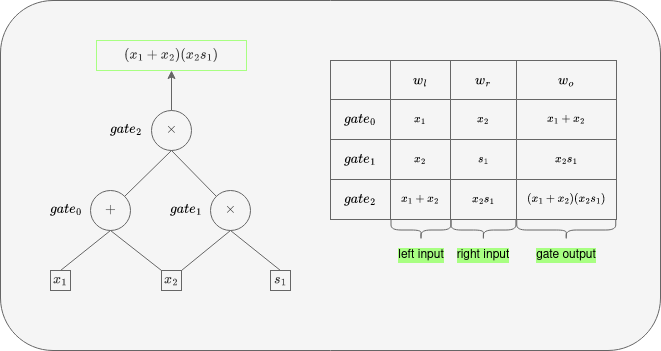
\includegraphics[width=1\linewidth]{figures/arithmetization.drawio.png}
    \caption{Toy Circuit}
    \label{fig:toy-circuit}
\end{figure}

The objective is to efficiently encode an arithmetic circuit into a set of polynomials. The first step is to encode each gate as an equation. Considering only gates for addition and multiplication, each gate could be written as one of the following:

\begin{align}
    \label{eq:primitive_gate_constraints}
    \text{\textit{addition:} } \text{left input} + \text{right input} = \text{gate output} 
    \\
    \text{\textit{multiplication:} } \text{left input} \times \text{right input} = \text{gate output}
\end{align}

That is a good start, but we could create an equation that can check the validity of both gate types. First, we denote the columns of the computational table as vectors $w_l, w_r, w_o$. By assigning $x_1 = 2, x_2 = 1, s_1 = 3$ for the \Cref{fig:toy-circuit} we get $w_l = [2, 1, 3], w_r = [1, 3, 3], w_o = [3, 3, 9]$. The values in the computation table represent the witness $(\publicinput, \witness)$, where $\publicinput$ are values of $x_1, x_2$ and the rest of the circuit is private $\witness$. 

To specify the type of the gate, we use selectors: $q_l$ left, $q_r$ right, $q_o$ output, $q_m$ multiplication, $q_c$ constant. These are vectors of size $n$ selecting the type of gate that we want to use. For example, if we are dealing with gate $i$, that is a multiplication gate, then $q_{m_i} = 1$; otherwise, it is always set to 0. The selectors could be combined to obtain the equation for gate $i$:

\begin{equation}
    \label{gate-constraint}
    w_{l_i}w_{r_i}q_{m_i} + w_{l_1}q_{l_i} + w_{r_i}q_{r_i} + w_{o_i}q_{o_i} + q_{c_i} + PI_i = 0
\end{equation}

Consider the example circuit and variable assignment $x_1 = 2, x_2 = 1, s_1 = 3$, and for simplicity, all unassigned selectors will have value 0. Then, it is possible to perform these operations:

\begin{itemize}
    \item \textit{addition:} $q_{l_i} = q_{r_i} = 1, q_{o_i} = -1$ \\
        For the addition gate, we want to keep only the addition and output terms of the equation. The rest will cancel out, thanks to the remaining selectors being 0.
    \item \textit{multiplication:} $q_{m_i} = 1, q_{o_i} = -1$ \\
        To engage a multiplication gate, we assign the selector such that only the multiplication and output terms of the equation remain.
    \item \textit{constant assignment:} \\
        Besides the operations of addition and multiplication, it is possible to do constant assignments (not illustrated on the example circuit). Say that we want the left input of a $gate_i$ to be equal to some constant $c$. To construct the equation for this gate, we can assign $q_{l_i} = 1, q_{c_i} = -c$, and the equation then simplifies to $w_{l_i} = c$, checking exactly what we want. This work, respectively, also for the right input, we just set the selectors as $q_{r_i} = 1, q_{c_i} = -c$.
\end{itemize}

$PI_i$ is public input, which is engaged only for the public input nodes (leaves of the graph). For all inner nodes, $PI_i = 0$. Notice that using the selector polynomial, some terms are canceled out so that we get to the separate gate constraints described in the beginning \eqref{eq:primitive_gate_constraints}. Below is a table with the explicit assignment of the selector for the specific example. 

% \begin{figure}[H]
%     \centering
%     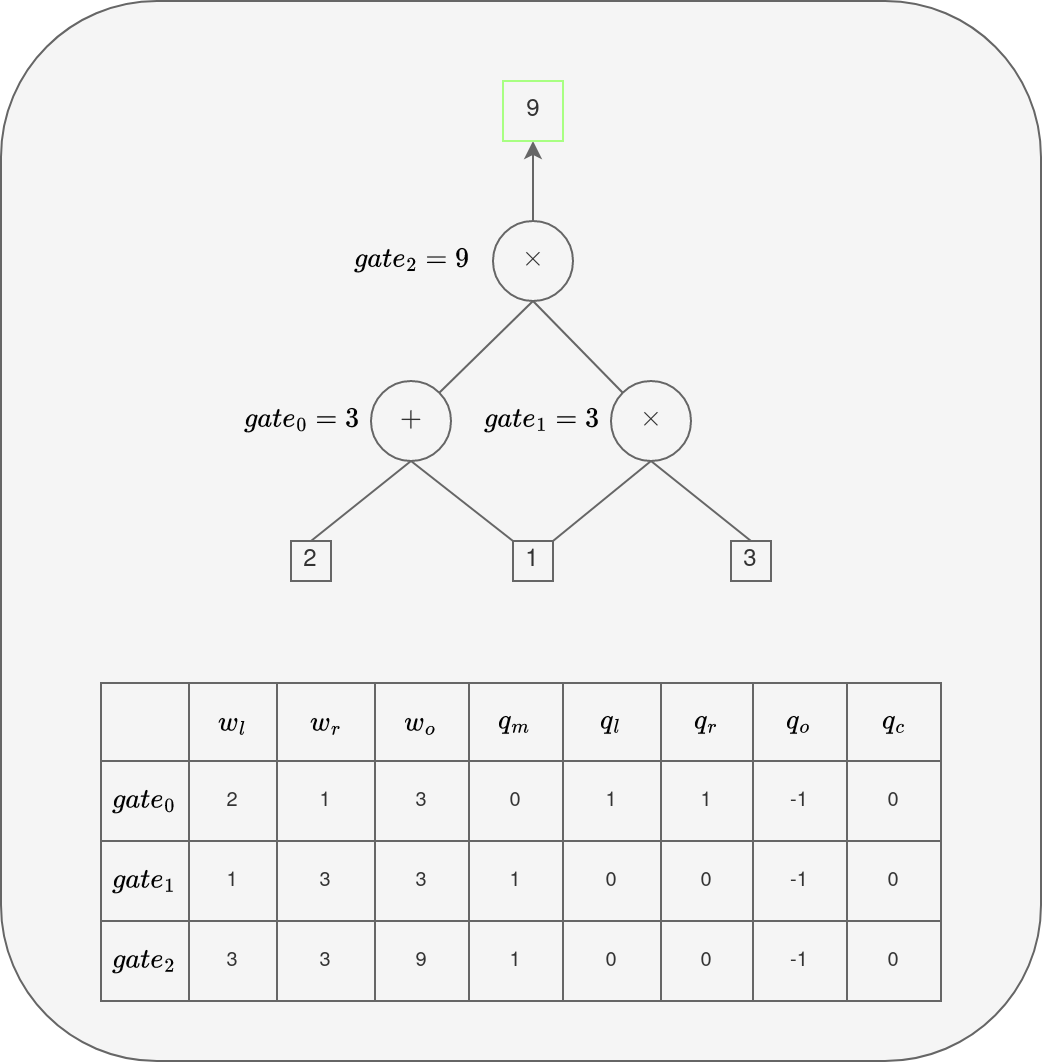
\includegraphics[width=0.75\linewidth]{figures/arithmetization_evaluated.drawio.png}
%     \caption{Evaluated diagram}
%     \label{fig:evaluated-circuit}
% \end{figure}

\begin{table}[H]
\begin{tabular}{|c|c|c|c|c|c|c|c|c|}
\hline
         & $w_l$ & $w_r$ & $w_o$ & $q_m$ & $q_l$ & $q_r$ & $q_o$ & $q_c$ \\ \hline
$gate_0$  & 2     & 1     & 3     & 0     & 1     & 1     & -1    & 0     \\ \hline
$gate_1$ & 1     & 3     & 3     & 1     & 0     & 0     & -1    & 0     \\ \hline
$gate_2$ & 3     & 3     & 9     & 1     & 0     & 0     & -1    & 0     \\ \hline
\end{tabular}
\end{table}

% Now we can get a bit closer to the arithmetization that is used in $\plonk$ we merge the witness vector $w_l, w_r, w_o$ into single $w$ such that: $$w_l = [w_0, \dots, w_{n-1}], w_r = [w_n, \dots, w_{2n-1}], w_o = [w_{2n}, \dots, w_{3n-1}]$$ 
% Now the witness $w$ encapsulates all of the values flowing through the circuit, where some of the values are public and some are secret. The verifier needs to check the output of the circuit and the public input, so naturally, these two will be public. The rest of the values remain private.

% To get the full gate equation we add one last thing. The public input to the circuit will be denoted by vector $PI$, remember that public input is a subset of the witness. In contrast to selector $q_c$, $PI$ can be changed for each execution of the circuit while 
% $q_c$ constants (surprisingly) remain bound to a specific circuit. For all (inner) nodes not related to input $PI$ will be set to 0. The full $\plonk$ gate equation looks like this:
% \begin{equation}\label{gate-constraint}
%     w_{i}w_{n+i}q_{m_i} + w_{i}q_{l_i} + w_{n+i}q_{r_i} + w_{2n+i}q_{o_i} + PI_i + q_{c_i} = 0 
% \end{equation}

% Let's revise this on our beloved Sudoku game. Imagine the prover is trying to convince the verifier that he knows the solution to a \href{https://en.wikipedia.org/wiki/Sudoku}{Sudoku problem}. Then the circuit is a program that checks if the Sudoku is filled validly and the prover wants to show that he can fill in such numbers that this program accepts his solution. Here the public input (public part of the witness) could be the initial state of the Sudoku problem as well as the dimensions of the board. Naturally private witnesses are the numbers that need to be filled in the board that the prover claims to know and does not want to share. We should also mention that there is a convention that the correct result of the circuit should be 0. That is the same as saying the output of the program is 0 if it succeeds.


\subsection{Transcription into polynomials}
It is possible to write express computation of each gate in the circuit as equation \Cref{gate-constraint}. But a much more elegant way is to condense all of the constraints into a single equation by interpolating the vectors.

\[
\begin{array}{cc}
    a(x) = \sum_{i=0} L_i(x)w_{l_i} & b(x) = \sum_{i=0} L_i(x)w_{r_i} \\
    c(x) = \sum_{i=0} L_i(x)w_{o_i} & q_l(x) = \sum_{i=0} L_i(x)q_{l_i}  \\
    q_{r_i}(c) = \sum_{i=0} L_i(x)q_{r_i} & q_m(x) = \sum_{i=0} L_i(x)q_{m_i}  \\
    q_{c_i}(x) = \sum_{i=0} L_i(x)q_{c_i} & PI(x) = \sum_{i=0} L_i(x)PI_i  \\
\end{array}
\]

This enables to represent gate constraints for the whole circuit $\CRKT$ as:
\begin{equation}
    \label{eq:gate-contraints}
    a(x)b(x)q_m(x) + a(x)q_l(x) + b(x)q_r(x) + c(x)q_o(x) + q_{c_i} + PI(x) = 0
\end{equation}

% This section was inspired by the lecture of Dan Boneh which is available on \href{https://zkhack.dev/whiteboard/}{ZK Whiteboard}. Since in the group of elliptic point we had only operation with addition and multiplication these will also be the only gates that we will use. Subtraction and division will be simulated by computing additive and multiplicative inverses. It is possible to work also with custom gates but for the simplicity this will be discussed in another section. For now we will consider only 2 binary gates. 

% Let's see how a specific circuit can be transformed into a polynomial. Take arithmetic operations $(x_1 + x_2)(x_2 + w_1)$ where $x$ are public inputs and $w$ is a secret witness. This can be visualized as a computation graph where the first sum is computed in addition $gate_0$, second sum in addition $gate_1$ and finally the product in $gate_2$.

% % \begin{table}[ht]
% %     \centering
% %     \begin{tabular}{ l | l l l}
% %      inputs:   & $x_1$ & $x_2$ & $w_1$       \\ 
% %      \hline
% %      $gate_0$: & $x_1$ & $x_2$ & $x_1 + x_2$ \\ 
% %      $gate_1$: & $x_2$ & $w_1$ & $x_2 + w_1$ \\ 
% %      $gate_2$: & $x_1 + x_2$ & $x_2 + w_1$ & $(x_1 + x_2)(x_2 + w_1)$ \\
% %     \end{tabular}
% %     \caption{Arithmetic circuit as a table}
% % \end{table}

% Notice how the first two columns show input and the third one output. The number in the right corner is 77 which is output of the arithmetic circuit. We set notation $|C|$ as number of gates in $C$, and also $|I| = |I_x| + |I_w|$ as number of public inputs plus number of private inputs. For case of binary gates the total number of elements in the computation trace is $d = 3|C| + |I|$ and we will also have set $\Omega = \{1, \omega, \omega^2, ..., \omega^{d-1} \}$. Now we are able to specify polynomial which partially represents the table. 

% In the original paper the each gate $i$ could be represented by a equation:

% $$q_{l_i} a_i + q_{r_i} b_i+ q_{o_i} c_i + q_{m_i} a_i b_i + q_{c_i} = 0$$

% where $a, b, c$ are left right and output wires and $q$ are selector polynomials. Specifically $q_l, q_r, q_o, q_m, q_c$ stand for left right output multiplication and constant, these are called selector and specify encode the structure of the circuit . Now for each gate we can perform three operations:
% \begin{itemize}
%     \item addition: by assigning 1 to selectors $q_l, q_r$, -1 to $q_o$ and 0 to remaining  
%     $a + b = c$
%     \item multiplication: by assigning 1 to $q_m$, -1 to $q_o$ and 0 to remaining $a \times b = c$
%     \item constant assignment: is done when binding to some public variable. we can bind it to the left variable by assigning $q_l = 1$, $q_c$ value we want to assign and rest is zero. $b = q_c$
% \end{itemize}

% \begin{table}[h]
%     \centering
%     \begin{tabular}{ l | l l l}
%      inputs:   & $t(\omega^{-1})= x_1$ & $t(\omega^{-2})=x_2$ & $t(\omega^{-3})=w_1$ \\ 
%      \hline
%      $gate_0$: & $t(\omega^{0})=x_1$  & $t(\omega^{1})=x_2$  & $t(\omega^{2})=x_1 + x_2$ \\ 
%      $gate_1$: & $t(\omega^{3})=x_2$  & $t(\omega^{4})=w_1$  & $t(\omega^{5})=x_2 + w_1$  \\ 
%      $gate_2$: & $t(\omega^{6})=x_1 + x_2$ & $t(\omega^{7})=x_2 + w_1$  & $t(\omega^{8})=(x_1 + w_2)(x_2 + w_1)$ 
%     \end{tabular}
%     \caption{Arithmetic circuit as a table}
% \end{table}

% % Now the polynomial will be interpolated. For example with FFT in time $d \log_2{d}$. This encoding has one flaw, can you spot it? We are not able to distinguish types of the polynomials and that is why we need selector polynomial. 

% To make this more succinct it would be nice to represent the whole circuit as a single polynomial. The key point to realize here is that system of equations in the same form could be interpreted as a single equation over polynomials. Suppose we have a vector like $v=(5,8,13)$. We can convert the vector into a list of points $(0,5),(1,8),(2,13)$ simply using the index of the value in the vector as the x-coordinate. Then there is a unique degree-2 polynomial function that passes through these points. Notice that we are entirely free to choose any domain we want. In $\plonk$ the polynomials are interpolated over the domain of roots of unity. The $n$-th root of unity is simply a group element that satisfies $x^n = 1$ and for $i<n, x^i \neq 1$. Let's have a set $\Omega = \{1, \omega, \omega^2, \omega^3 ..., \omega^n-1\}$

% To make this complete we need to realize that gate wire constraints $a, b, c$ are different for each of the equation and we can just transform them to polynomial to arrive to:
% $$L(x)a(x) + R(x)b(x) + O(x)\CRKT(x) + M(x)a(x)b(x) + O(x) + \CRKT(x) = 0$$


% By transcribing the problem we are reinterpreting the problem in terms of polynomial. We are asking the prover to give us witness $w$ such that together with the public input $x$ a specific program encoded circuit $C$ will give out some value. In the general case we are asking for such $w$ that $\CRKT(x,w) = 0$. Right now we will consider gates just with standard group operations. By that we mean addition and multiplication. In later sections we will see that it is also possible to construct $\plonk$ with custom gates, for now we will make our life easier by dealing only with binary gates.

% During the process of arithmetization the the $\verifier$ needs to make sure that $\prover$ did not cheat in any way. In particular we need to have gate constraints, which are equations between wires that are attached in the same gate. Secondly we will also want to have copy constraints that guarantee that for two consecutive gates the output of the first one is input to the second one. 


 
%%%  ===========================================================================
\section{Circuit checks}
\label{sec:checks}
We can encode arbitrary circuits with polynomials. The following objective is to convince the verifier that the prover knows such a secret witness $\witness$, for which $\CRKT(\publicinput, \witness) = 0$. The prover needs to guarantee the integrity of computing the circuit, and it turns out the verifier needs a lot of convincing since there are numerous ways to cheat. The prover needs to show that the following:
\begin{enumerate}
    \label{plonk-checks}
    \item correct public inputs are provided (input check)
    \item Gates are computed correctly (gate check)
    \item Gates are wired correctly (wiring check)
    \item The output of the circuit is zero (output check)
\end{enumerate}

Most of the checks are descriptive, besides the wiring check. Considering the example circuit \eqref{fig:toy-circuit}, this check ensures that outputs of $gate_0, gate_1$ are indeed provided as inputs to $gate_2$. This is also referred to as copy constraints because we want to make sure that the output of some gate is correctly copied to the input of another gate. Before proceeding to the implementation of this check, we will show how to perform zero tests on some domains.

\subsection{Zero Test}
\label{zero-test-on-h}

Observe that if some polynomial $f(x)$ is zero on $H$, then every element of $H$ has to be its root. A polynomial that has roots in all elements of the domain was denoted as $Z_H(x)$. That means we can factor the polynomial as $f(x) = g(x)Z_H(x)$. Therefore, if a polynomial is zero on $H$, it has to be divisible by the vanishing polynomial $Z_H(x)$. 

To put this into context, this test can be made into a standalone protocol with a polynomial commitment scheme. Below is a sketched diagram of how it works. In the $\plonk$ protocol, we will use this check, but the zero checks are not run independently on each polynomial. Instead, they are batched into the quotient polynomial $t(x)$ in \Cref{chap:round3}.

% % \pseudocodeblock{
% %   \textbf{Prover} \< \< \textbf{Oracle} \< \< \textbf{Verifier} \\
% %   \text{work} \< \< \< \< \\
% %   p(x), q(x) = p(x) / Z_H(x) \< \< \< \< \\
% %   \text{Add to transcript} \< \< \< \< \\
% %   \< \sendmessageright{top=transcript} \< \< \< \\
% %   \< \< z \gets \mathbb{F}_p \< \< \\
% %   \< \sendmessageleft{top=z} \< \< \< \\
% %   \< \sendmessagerightx{8}{p(z), q(z)} \< \\
% %   % \< \< \< \sendmessageright{top=Work result, bottom=Bottom message} \< \\
% %   \< \< \< \< \text{work} \\
% %   \< \< \< \< \text{verify KZG evaluation} \\
% %   \< \< \< \< Z_H(z) = z^n - 1 \\
% %   \< \< \< \< p(z) \stackrel{?}{=} q(z)Z_H(z) \\
% % }


% % %   \< \sendmessageright{top=transcript} \< \< \< \\
% % %   \< \< z \gets \mathbb{F}_p \< \< \\
% % %   \< \sendmessageleft{top=z} \< \< \< \\


% \begin{enumerate}
% \label{plonk-checks}
%     \item $P$ correctly encodes all of the inputs (input check)
%     \item Gates are computed correctly (gate check)
%     \item Gates are wired correctly (wiring check)
%     \item The output of the circuit is zero (output check)
% \end{enumerate}

% % % \hl{why is the input chosen such that the output is zero}

% Let $\omega \in \mathbb{F}_p$ be a primitive $k$-th root of unity for which $\omega^k = 1$. Then we can define a set $\Omega = \{1, \omega, \omega^2, ... \omega^{k-1}\}$ and $f \in \mathbb{F}_p^{\leq d} (X)$. Now there are some tasks, that prove might want to show to the verifier. Especially we will be interested into zero-test which shows that $f$ is identically zero on the set $\Omega$. This test uses a simple algebra fact:

% \begin{lemma}
%     $f$ is zero on $\Omega$ if and only if $f$ is divisible by $(x^k - 1)$
% \end{lemma}

% \begin{proof}
%     Let's start with reverse implication $\leftarrow$. If $f$ is divisible by $(x^k - 1)$ that means it can be factored into $f(x) = g(x)(x^k - 1)$. Now what happens if we plug some value of $\Omega$ into the function? For 1 it is obvious that the polynomial will result to zero and for others can be considered as $\omega^i, i<k$. Now using that fact that $\omega^k = 1$:
%     $$(x^k - 1) = ((\omega^{i})^k - 1) = ((\omega^{k})^i - 1) = (1^i - 1) = 0$$
    
%     $\rightarrow$ if $f$ is zero on $\Omega$ than plugging in any $\omega^i \in \Omega$ should result in zero and that is achieved when $f$ is divisible by $(x^k - 1)$ as seen in the previous case.
% \end{proof}

% This test can be transformed in a scheme. The prover would compute $q(x) = \frac{f(x)}{(x^k -1)}$ and will commit to $f, q$ using polynomial commitment scheme, which could be KZG. Then the verifier will sample a random $r \in \mathbb{F}_p$ and ask for evaluation of $f(r), q(r)$, the resulting verification will just compare: $f(r) = q(r)(r^k - 1)$. By % % \hl{lemma x} the probability that these polynomials are identical based on evaluation of a single point is sufficient. The verifier needs to compute $r^k$ which can be done in $O(log k)$

% Besides that a product check would be also very useful for us: $c = \prod_{\omega \in \Omega} f(\omega)$

% % % \hl{Perhaps add diagram for zero test}


\pseudocodeblock[head=Zero test]{
    \text{Prover } \prover \< \< \text{Verifer } \verifier \\
    \< \< \\[-0.5 \baselineskip]
    f(x), g(x) = f(x) / Z_H(x) \< \sendmessageright*{\relax[f]_1, [g]_1} \< \< \\
    \< \sendmessageleft*{z} \< z \gets \field \\
    \text{evaluate } f(z), g(z) \< \< \\
    \text{compute opening proofs } \pi_1, \pi_2 \< \< \\
    \< \sendmessageright*{f(z), g(z), \pi_1, \pi_2} \< \\
    \< \< \text{verify KZG openings } \pi_1, \pi_2 \\
    \< \< Z_H(z) = z^n - 1 \\
    \< \< f(z) \stackrel{?}{=} g(z)Z_H(z)
}

\begin{theorem}
    Zero-test is correct and computationally sound, assuming $\frac{d}{p}$ is negligible.
\end{theorem}

\label{is this sufficient?}
\begin{proof}
    We have already discussed the properties of KZG in \cref{chap:kzg} and the Schwartz-Zippel lemma in \Cref{comparing-poly}. 

    This check satisfies correctness because if $f(x)$ is zero on $H$, then it can be factored into $Z_H(x)g(x)$. The verifier can check the KZG opening and compare polynomials using the Schwartz-Zippel lemma.

    The zero test is also computationally sound because if the polynomial $f(x)$ is
    not zero on the whole domain $H$, then it cannot be divided by $Z_H(x)$. As a result, the prover cannot provide $g(x)$ that would satisfy $f(z) = g(z)Z_H(z)$ with non-negligible probability, which follows from the Schwartz-Zippel lemma.
\end{proof}


\subsection{Output Check}
Notice that the output of the circuit is always the output of the last gate of the circuit. This means the output of the circuit will be encoded as the last element of the witness. All the prover needs to do is show that $\CRKT(\omega^{n-1}) = 0$. This can be performed in a secure way using a polynomial commitment scheme where the verifier asks to open the polynomial $c(x)$ at $\omega^{n-1}$.

\begin{lemma}
    \label{output-correctness-soundness}
    The output check is correct and sound.
\end{lemma}

The properties of this check depend on the polynomial commitment scheme, and we have already discussed the validity of KZG in \Cref{chap:kzg}.

\subsection{Gate Check}
We have managed to encode the gate constraints by the equation  \Cref{eq:gate-contraints}. Using the zero test, it is possible to verify that $\forall x \in H:$
$$a(x)b(x)q_m(x) + a(x)q_l(x) + b(x)q_r(x) + c(x)q_o(x) + q_{c_i} + PI(x) = 0$$


\begin{lemma}
    \label{gate-correctness-soundness}
    The gate check is correct and computationally sound
\end{lemma}

\begin{proof}
    This follows from the properties of the zero test \Cref{zero-test-on-h}
\end{proof}

\subsection{Input Check}
We have encoded the public input is encoded using \Cref{eq:gate-contraints}. That means checking if correct public inputs were provided to the circuit can be encoded in the gate equation.

\begin{lemma}
    \label{input-correctness-soundness}
    The public input check is correct and sound
\end{lemma}

This follows from \Cref{gate-correctness-soundness}.

\subsection{Wiring Check}
\label{sec:wiring-check}
The structure of a circuit requires some values to be identical. The edges (wires) indicate that the output of the gate at one side should be passed as the input to the other gate. To ensure that the program is computed correctly, the prover needs to show that the values were copied correctly.

This check is performed using permutations. The structure of the circuit induces some equivalence classes. We will try to show that the copy constraints are satisfied by performing a permutation on the equivalence classes. For this purpose, we will choose rotation because it changes the position of every element. The diagram below \Cref{fig:permutation-function} shows how the permutation function would look for \Cref{fig:toy-circuit}.

\begin{figure}[H]
    \label{fig:permutation-function}
    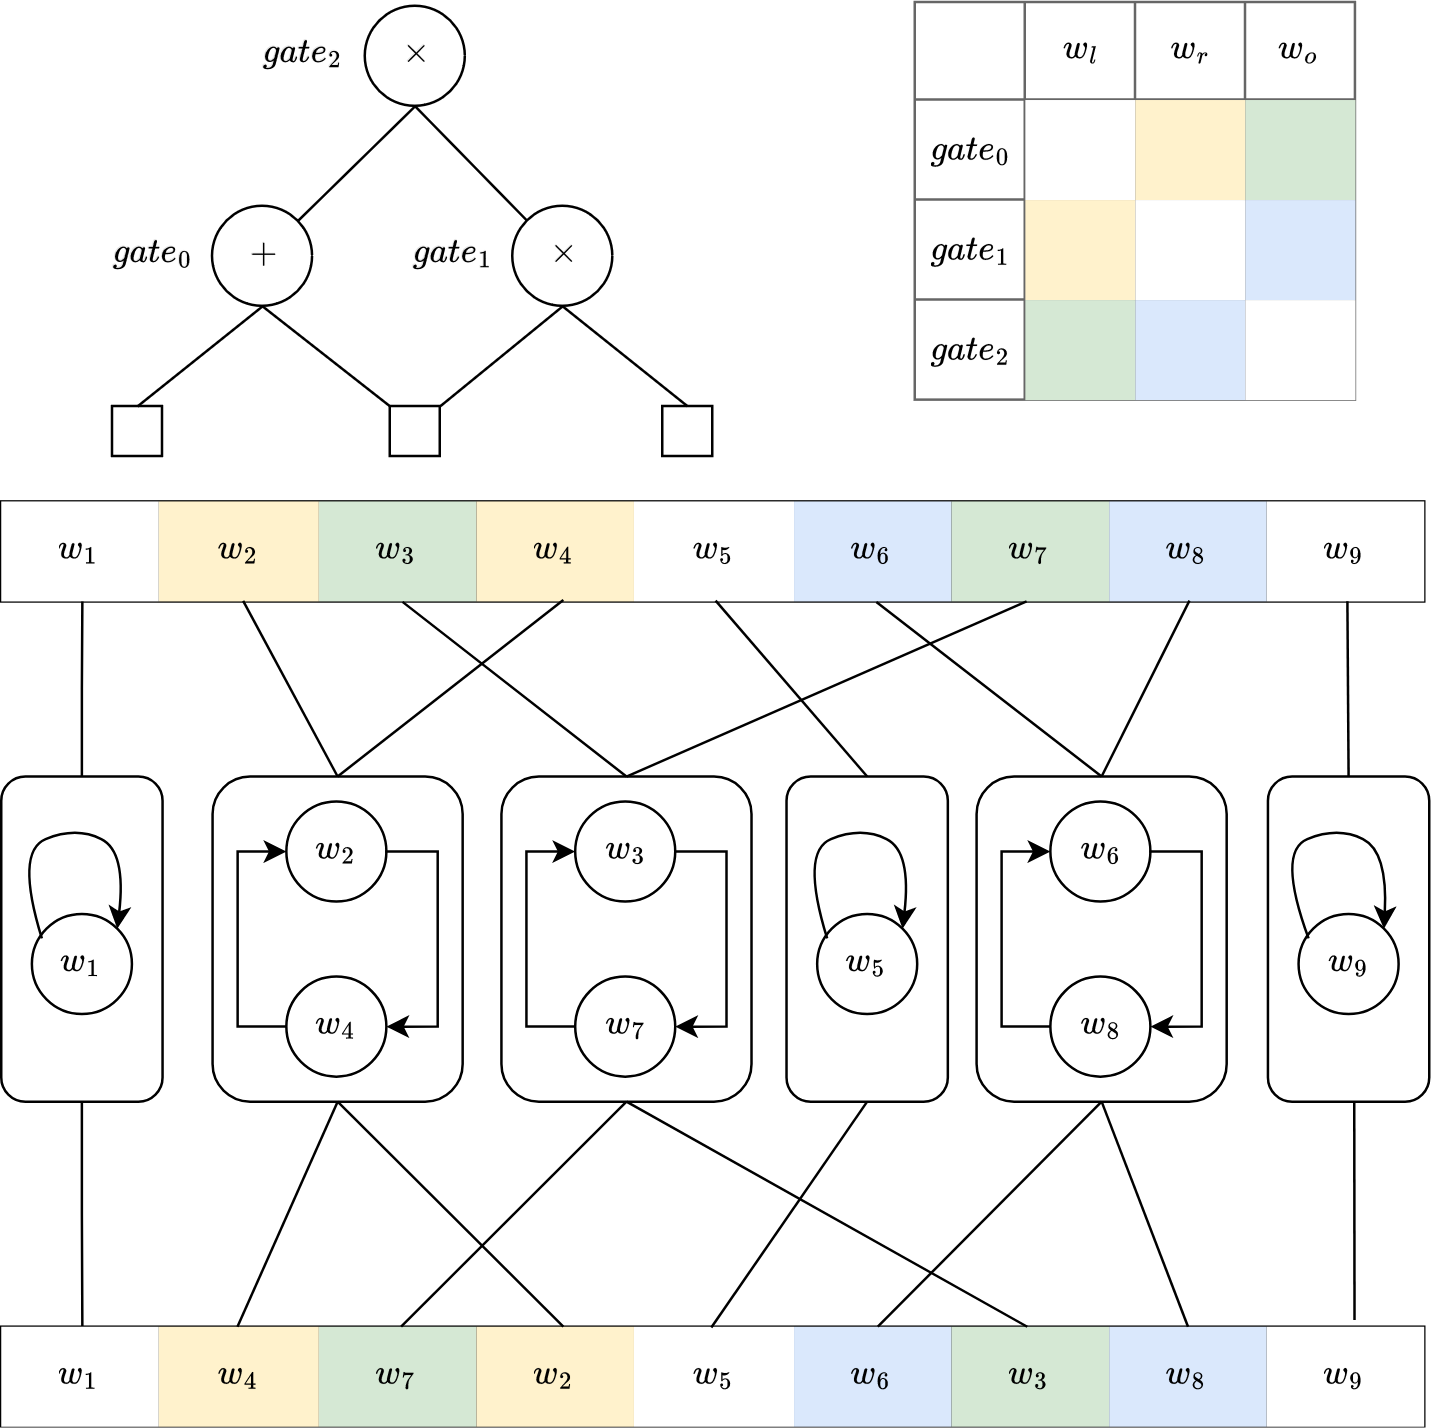
\includegraphics[width=0.75\linewidth]{round-figures/round2/permutation_function.drawio.png}
    \caption{Rotation of equivalence classes}
\end{figure}

It might look complicated, but essentially, we just did a clockwise rotation on the groups of variables of the circuit. Since we have changed the variables with equal values, the circuit should work the same as before and produce the same output. If all of the gate equations were true before the shuffling, then they would succeed also after this shuffling. On the other hand, if the prover did not do the arithmetization correctly and the gate wiring is not the same as in the former circuit, this check would detect it (with very high probability). That is the core idea that will be used in the permutation check.

\begin{lemma}
    \label{permutation-correctness-soundness}
    Consider vector $v = [v_1, v_2 \ldots v_n]$, constraints $v_i = v_j, v_k = v_l \ldots$ and a permutation function $\sigma$ that permutes the equivalence classes determined by the constraints. All of the contains are satisfied if and only if $v = \sigma(v)$.
\end{lemma}

\begin{proof}
    \textcolor{white}{there is nothing on this line:)}
    
    \begin{enumerate}
        \item[$\Rightarrow$] If all of the contains are satisfied and $\omega$ permutes only the indices inside the permutation classes, then the values remain unchanged. 
        \item[$\Leftarrow$]  If the vector remain unchanged after performing the permutation $\sigma$ then all of the elements in the equivalence classes induced by the permutation function must be the same and thus the constraints hold.
    \end{enumerate}
\end{proof}


\chapter{PLONK Rounds}

Now that we finally have all of the components needed let's construct the protocol. The $\plonk$ protocol has a one-time trusted setup algorithm that generates the common preprocessed input. Part of this setup is to generate the \textit{structured reference string} for polynomial commitments. The prover has a routine proving algorithm that is split into 5 rounds in the original paper, this is the approach we will take as well. Finally, there is an algorithm for the verifier, that is very much implicit. There will be a provided diagram to show how the protocol works. Below is the legend for these diagrams.


\begin{figure}[H]
    \centering
    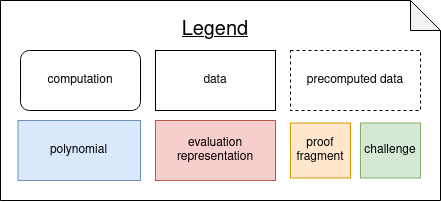
\includegraphics[width=0.5\linewidth]{round-figures/legend.drawio.png}
    \caption{Legend for the Plonk diagrams}
    
\end{figure}



\begin{figure}[ht]
    \centering
    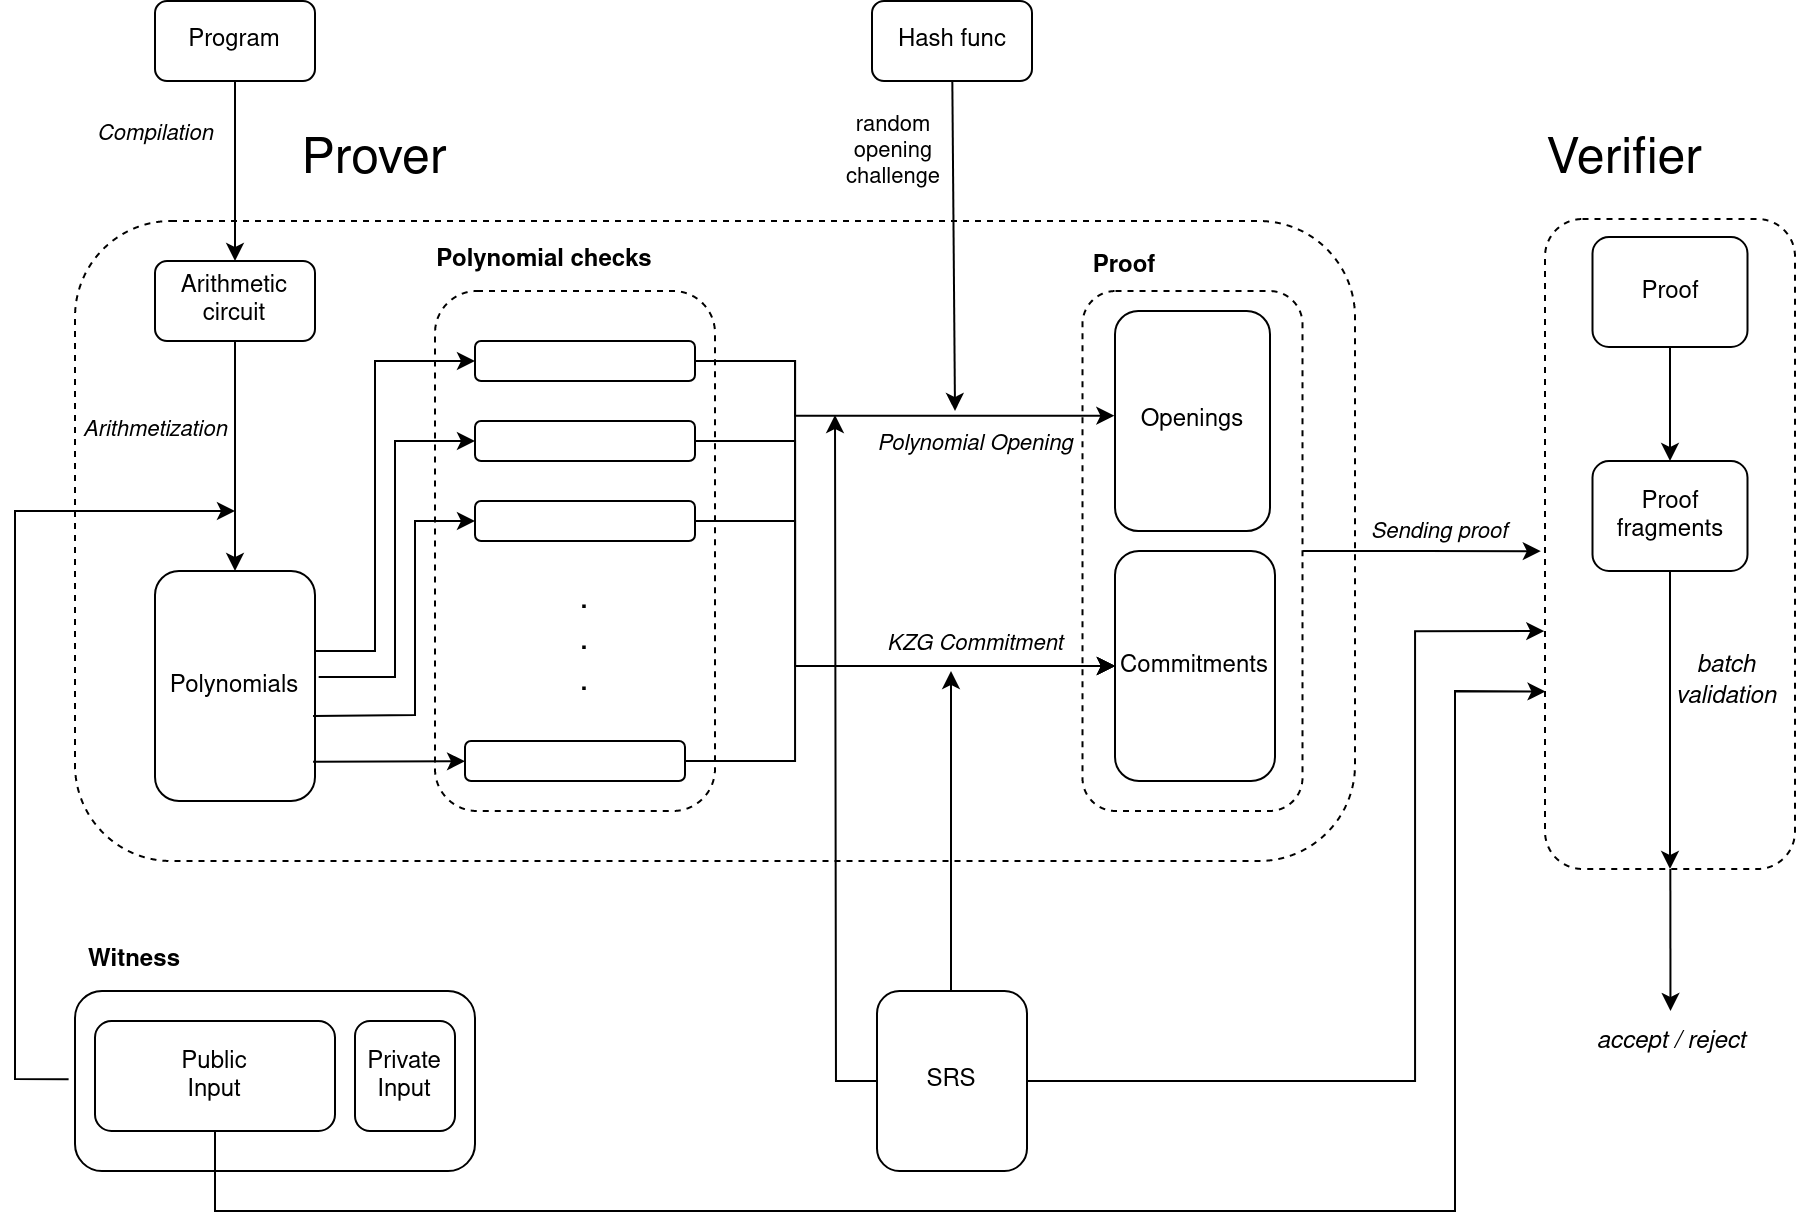
\includegraphics[width=1\linewidth]{round-figures/round1/plonk_better_overview.drawio.png}
\end{figure}

Throughout reading the protocol keep in mind that we will be aiming for following complexities:
\begin{itemize}
    \item proof size: $O(\log{d})$
    \item verifier time: $O(\log{d})$
    \item prover time: do not know need to find
\end{itemize}

% ==============================================================================
% ===SETUP======================================================================
% ==============================================================================
\section{Setup algorithm}
\label{chap:round0}
The setup algorithm describes the calculation of the common pre-processed input. It is not considered a routine protocol round. The only trusted part is the public key \textit{structured reference string} $SRS$ that is not tied to the structure of an arithmetic circuit but to the upper bound of the number of the circuit gates. This means that the circuit could be updated without the need to perform a trusted setup and $SRS$ can be reused. It is important to note that the $SRS$ cannot be generated by the prover because discovering the key $\tau$ would allow one to forge commitments and therefore give invalid evaluations.

\begin{figure}[H]
    \centering
    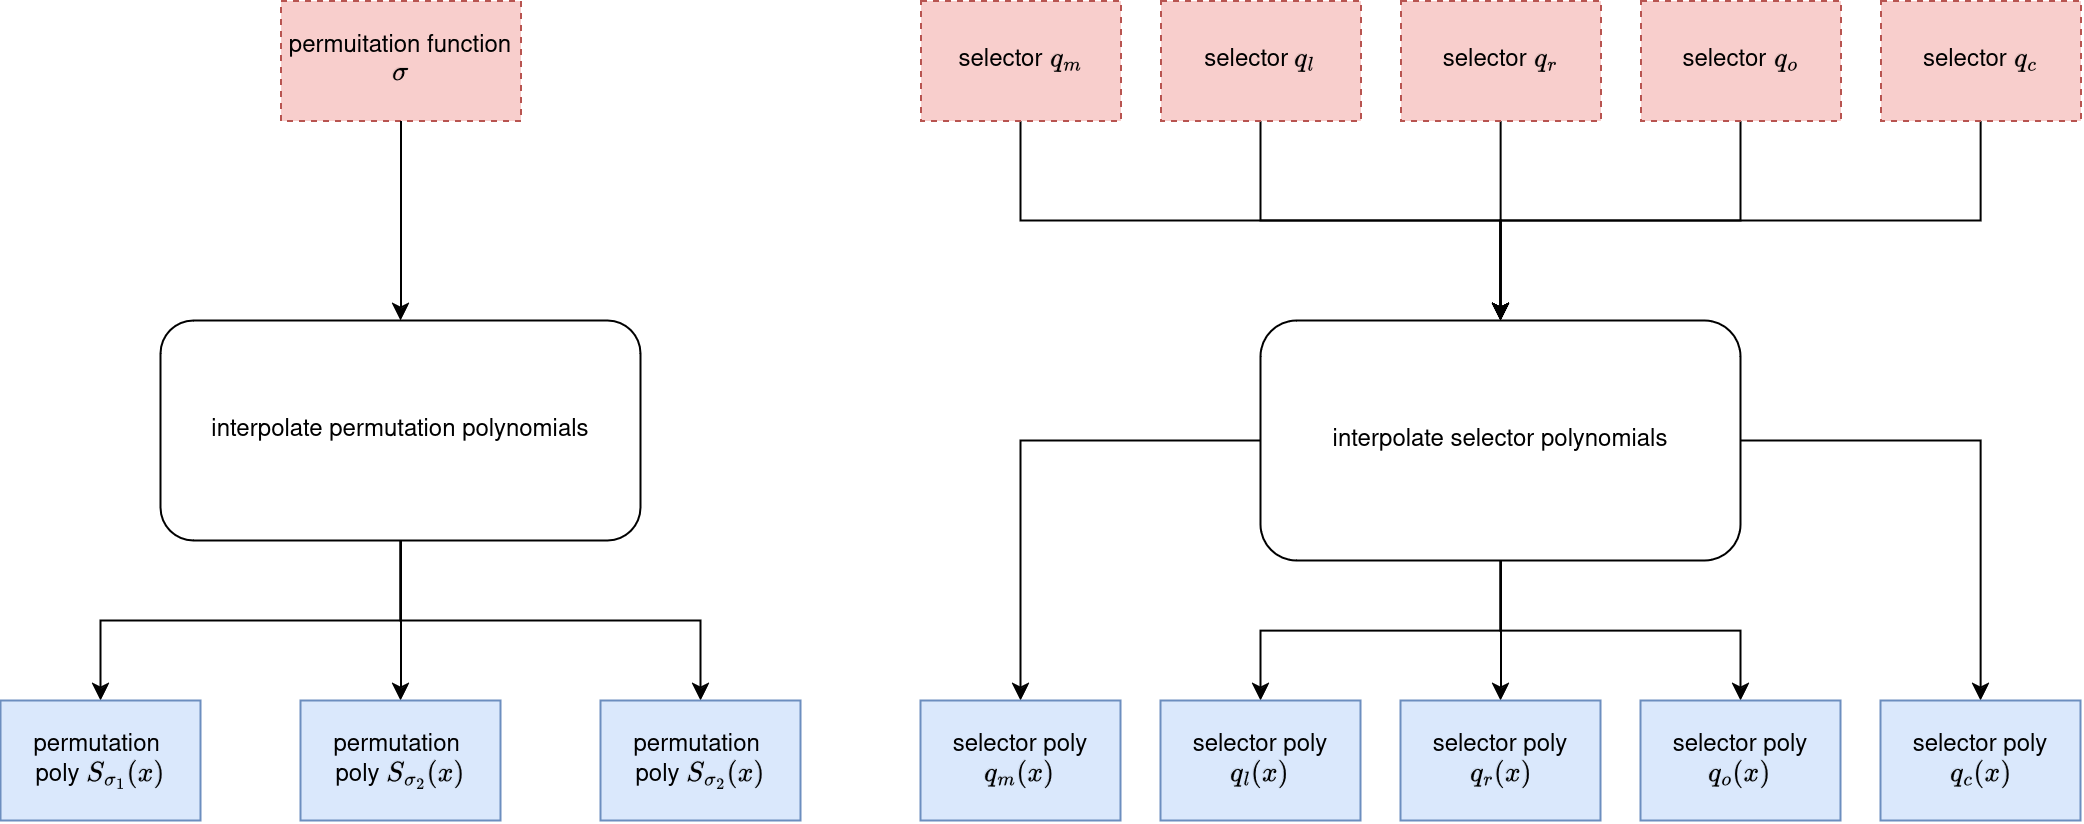
\includegraphics[width=1\linewidth]{round-figures/setup/round0.drawio.png}
    \caption{Setup algorithm}
    
\end{figure}


\subsection{Public Information }
All of the parties have information $(\field, \mathbb{G}_1, \mathbb{G}_2, \mathbb{G}_t, e, G_1, G_2, G_t, SRS)$ where $\field$ is a prime field, $(\mathbb{G}_1, \mathbb{G}_2, \mathbb{G}_t)$ are groups of points on elliptic curves and $e$ is efficiently computable group pairing $e: \mathbb{G}_1 \times \mathbb{G}_2 \rightarrow \mathbb{G}_t$. Lastly $G_1, G_2$ are group generators for which holds $e(G_1, G_2) = G_t$. All of the information above needs to be available to any party to perform arithmetic operations on elliptic curves. Moreover, there needs to be a KZG setup ceremony generating the \textit{structured reference string} SRS which is public.

Some input to the circuit might be public. This means we are able to split the witness $w$ into public $w_{pub} = (w_i)_{i\in [l]}$ and private $w_{priv} = (w_i)_{i = l+1}^{3n}$ where $l < n$ is the number of public inputs to the circuit. The public input is encoded as a polynomial:
$$PI(x) = \sum_{i \in [l]} - w_{pub_i} L_i(x)$$


\subsection{Preprocessed Input}
Below is summed up the common preprocessed input that is available to both parties. Each of the components will be described in detail in the following rounds.

\begin{itemize}
    \item number of gates: $n$
    \item $k_1, k_2 \in \field$ are needed to create cosets $k_1 H , k_2 H$ of group $H$ such that the union $H' = H \cup k_1 H \cup k_2H)$ contains $3n$ distinct elements. This will be explained in the round 2.
    \item $SRS$ for KZG: $([1]_1, [\tau]_1, [\tau^2]_1, ..., [\tau^{n+5}]_1, [1]_2, [\tau]_2)$ 
    \item permutation function: $\sigma^*: [3n] \rightarrow H'$ 
    \item selector polynomials: $q_m(x), q_l(x), q_r(x), q_o(x), q_c(x)$ interpolated from selector vectors explained in arithmetization
    \item permutation polynomials: $S_{\sigma_1}, S_{\sigma_2}, S_{\sigma_3}$ interpolated from $\sigma^*$ in detail in round 2
\end{itemize}


% ==============================================================================
% ===ROUND1=====================================================================
% ==============================================================================
\section{Round 1}
\label{chap:round1}

The proof generation starts by computing the wire polynomials and committing to them. In this chapter, we will also explain:

Round overview:
\begin{enumerate}
    \item Generate random blinding scalars $(b_1, ... b_9) \in \field$ just some numbers needed to introduce randomness 
    \item Compute wire polynomials $a, b, c$
    \item Compute and output commitments $[a]_1, [b]_1, [c]_1 \in \mathbb{G}_1$ 
\end{enumerate}

\begin{figure}[H]
    \label{fig:round1}
    \centering
    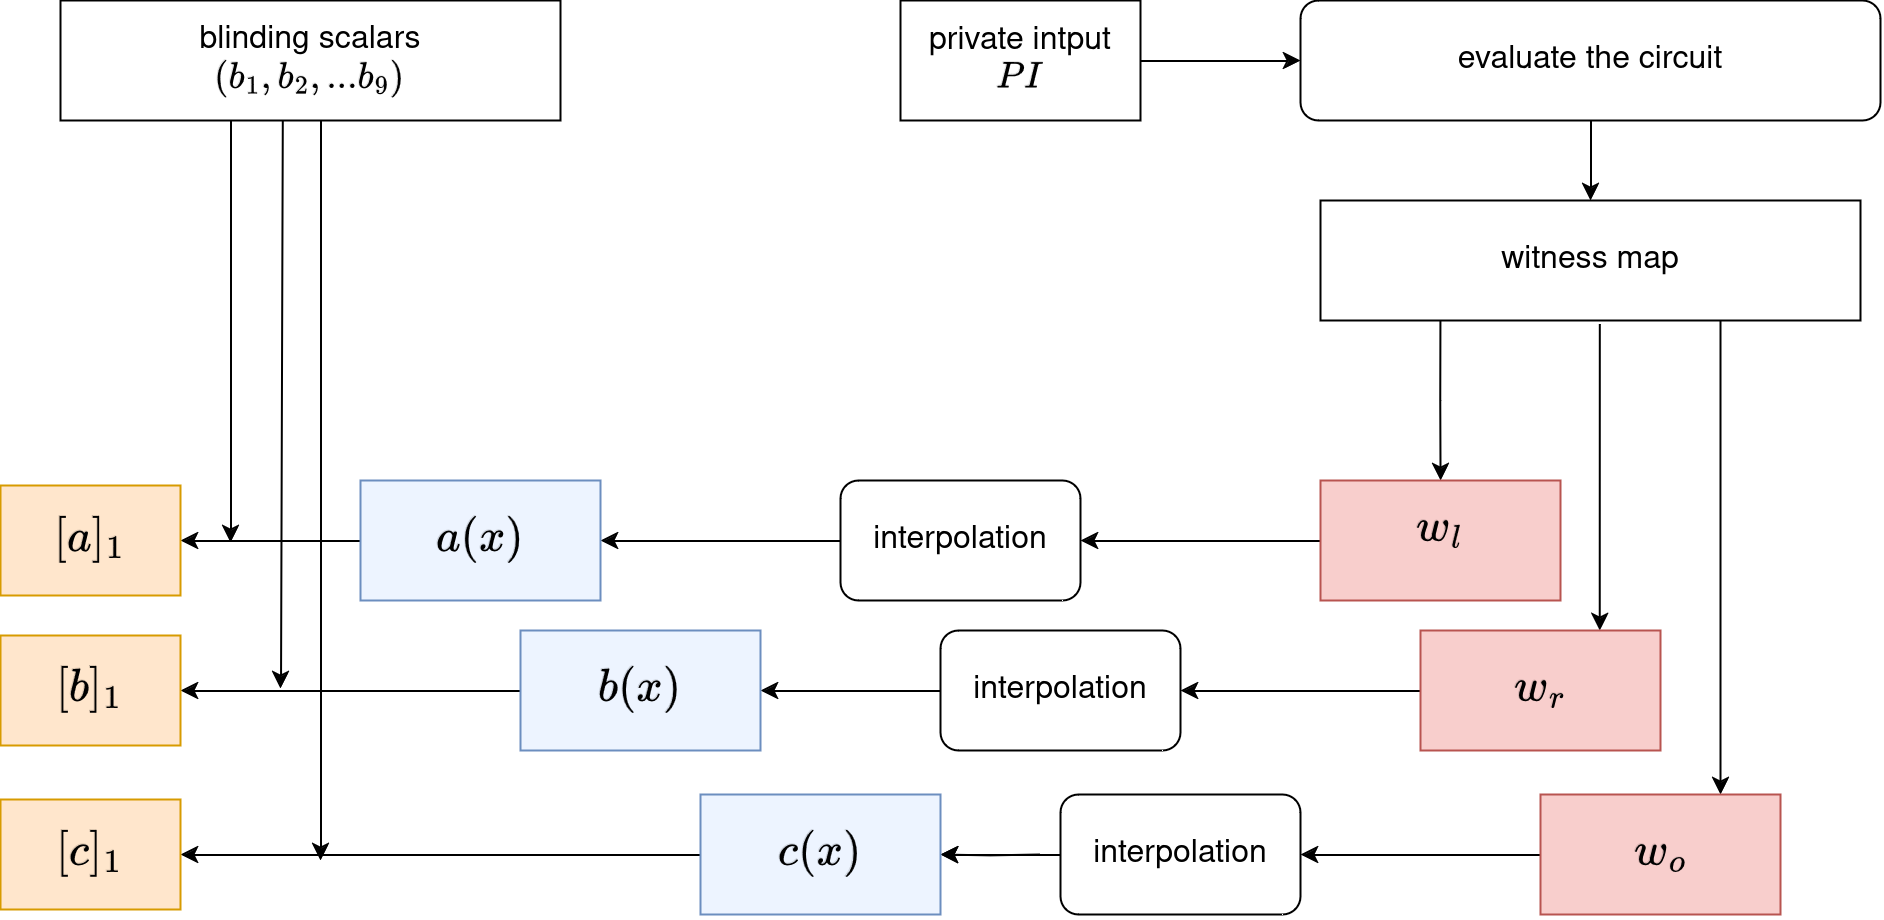
\includegraphics[width=1\linewidth]{round-figures/round1/round1.drawio.png}
    \caption{Round 1 Diagram}
\end{figure}


% \begin{note}[Intuition on why does this maintain the zero-knowledge property?]
%     Assume that the challenges for openings $z_1, z_2, \ldots, z_k$ are not in $H$ so $Z_H$ does not vanish on any of the challenges. The zero-knowledge (insanely informally) suggests that looking at the openings $p'(z_i)$ should give no information about $p(z_i)$. To the verifier openings, $p'(z_i)$ should look like uniformly randomly selected numbers. If there was any pattern in the openings the pattern might provide some (perhaps useful) information about the secret polynomial $p$. 

%     Take $b_1 + b_2x + b_2x^2 ... + b_{k+1}x^{k}$ as a blinding polynomial. Then the opening polynomial could be written as $p'(x) = b(x)Z_H + p(x)$. Now we notice that each set of openings $p'(z_1), p'(z_2), p'(z_3), \ldots p'(z_k)$ produces unique blinding polynomial. We take as a fact that a polynomial of degree $k$ is uniquely defined by $k+1$ points. This means that the polynomial $b(x)$ could be constructed by interpolating points: $\{(z_1, b(z_1)), (z_2, b(z_2)), (z_3, b(z_3)) \ldots, (z_k, b(z_k))\}$ form  $$b(z_i) = \frac{p'(z_i) - p(z_i)}{Z_H}$$

%     The last step is to realize that if we fix the secret polynomial $p(x)$ then by choosing the blinding polynomial we could get just about any set of opening points. Given that the coefficients of the blinding polynomial were chosen independently uniformly randomly we can say that the set of opening points $p'(z_1), p'(z_1), p'(z_1), \ldots, p'(z_k)$ produces also uniform distribution. Keep in mind that this trick only works if the blinding polynomial has a sufficient degree.
% \end{note}



\subsection{Computing wire polynomials}
Remember that we got the witness values in the arithmetization as columns of the computational table. The domain is chosen as $H = \{1, \omega, \omega^2, \ldots, \omega^{n-1}\}$ where $\omega^n = 1$. Choosing such a domain allows for a sparse representation of the vanishing polynomial as $Z_H(x) = x^n -1$ based on \cref{lemma:vanishing-poly}.

By pairing this domain with the witness $w$ we get the wire polynomials in the evaluation domain. To make commitments the polynomial needs to be in the coefficient form to evaluate it at the point $\tau$. Conversion to the coefficient form can be achieved by applying the Lagrange interpolation.

Finally, to make sure that the commitment to the wire polynomials does not leak information about the wire polynomial, they should be blinded. As described in \cref{theorem:blinding} this construction maintains the zero-knowledge property. The prover needs to uniformly randomly sample 9 blinding scalars $(b_1, b_2, \ldots, b_9)$. In round 1 there are sampled 9 blinding scalars, even though we only need 6. The remaining will be used in the next rounds.

\procedureblock[linenumbering]{$Round1_{\prover}$}{
    (b_1, \ldots, b_9) \sample \field^9 \\
    a(x) = (b_1x + b_2)Z_H(x) + \sum_{i=0}^{n-1} w_i L_i(x) \\
    b(x) = (b_3x + b_4)Z_H(x) + \sum_{i=0}^{n-1} w_{n+i} L_i(x) \\
    c(x) = (b_5x + b_6)Z_H(x) + \sum_{i=0}^{n-1} w_{2n+i} L_i(x) \\
    \pcreturn [a]_1, [b]_1, [c]_1
}


% ==============================================================================
% ===ROUND2=====================================================================
% ==============================================================================
\section{Round 2}
\label{chap:round2}

In this round awaits a big challenge - ensuring copy constraints of the circuit. We will see how it is possible to ensure the wiring constraints thanks to clever tricks. We will start by ensuring that constraints hold for inter-vector checks and then extend it to intra-vector checks.

Round overview:
\begin{enumerate}
    \item Receive permutation challenges $(\beta, \gamma) \in \field$ from the prover
    \item Compute permutation polynomial $z(x)$
    \item Compute and output commitment $[z]_1 \in \mathbb{G}_1$
\end{enumerate}

\begin{figure}[H]
    \centering
    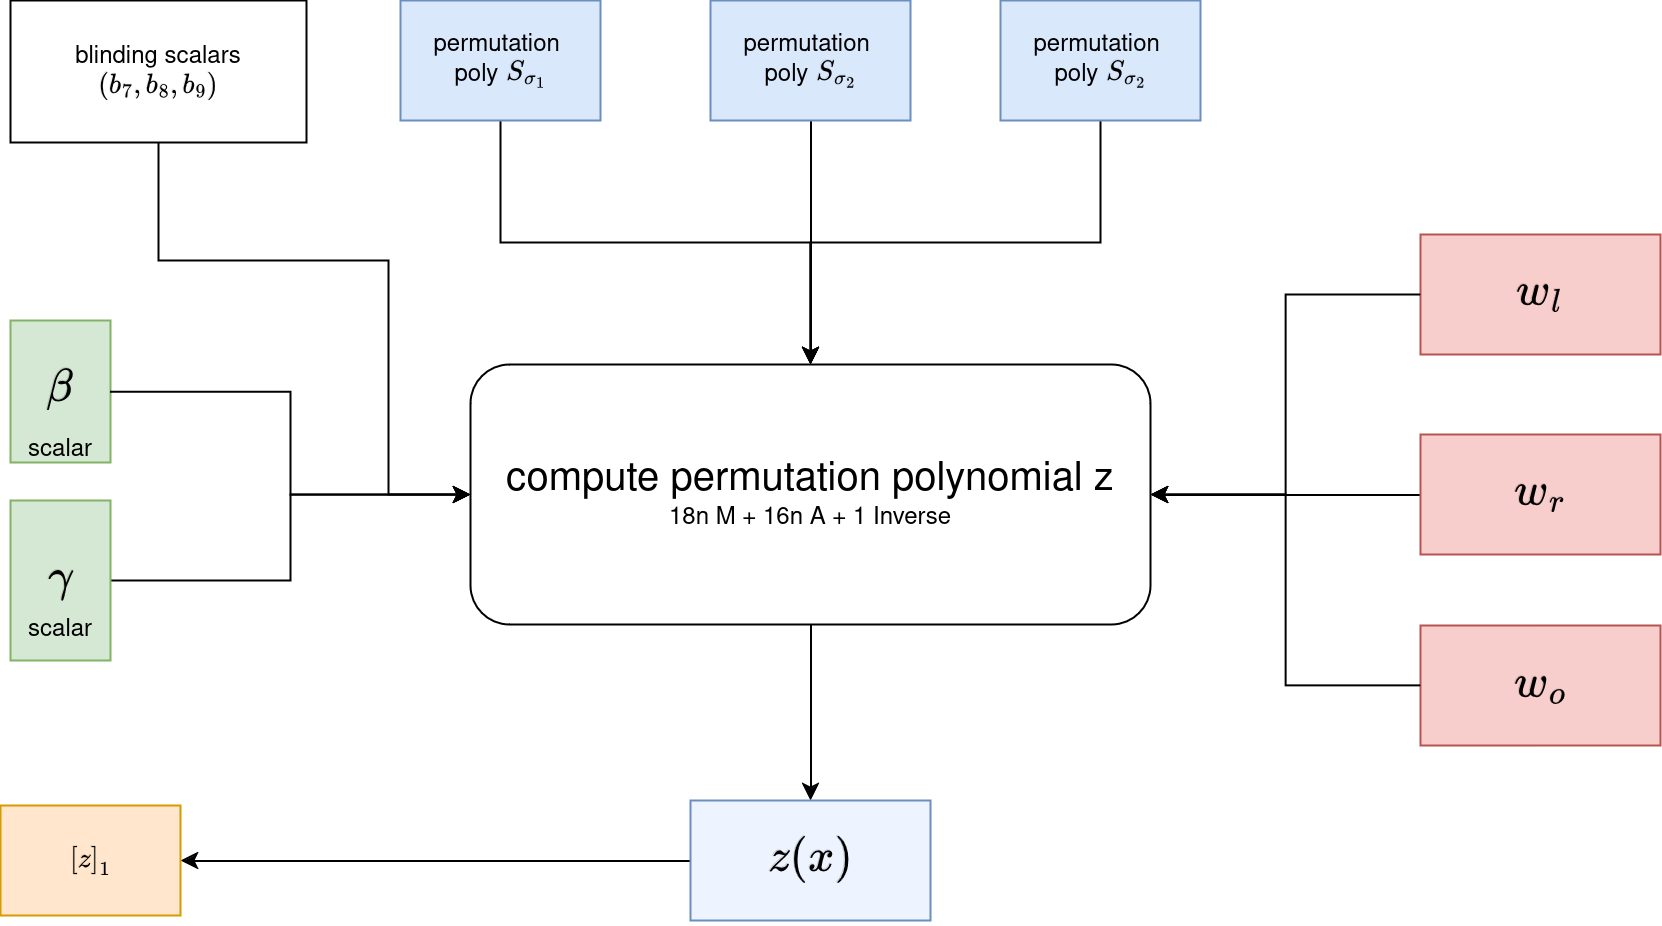
\includegraphics[width=1\linewidth]{round-figures/round2/round2.drawio.png}
    \caption{Round 2 Diagram}
    \label{fig:round2}
\end{figure}




\subsection{Intra-vector check}
We already know that the wire check could be efficiently checked by applying a suitable permutation function. Now we would like to show that this function indeed is a permutation and maintains the form of the vector. Given vectors $w$ and permutation function $\sigma$ we would like to efficiently verify that $\sigma$ is permutation. The brute-force approach has complexity $\bigO{n^2}$, on the other hand, naive approaches like performing sum checks are not reliable enough. Instead, the check could be performed by sampling uniformly random element $\beta$ and verifying $(w_1 + \beta)\ldots(w_n + \beta) \stackrel{?}{=} (\sigma(w_1) + \beta)\ldots(\sigma(w_n) + \beta)$. The trick is to think about these terms as polynomials with variable $\beta$, then we could use the theorem about polynomial intersection.

\begin{lemma}
    For vector $w$ of size $n$ and a function $\sigma$ of degree $n$ it is possible to verify that $\{w_1, w_2, \ldots, w_n\} \stackrel{?}{=} \{\sigma(w_1), \sigma(w_2), \ldots, \sigma(w_n) \}$ by $\prod_{i=0}^n (w_i + \beta) \stackrel{?}{=} \prod_{i=1}^n (\sigma(w_i) + \beta)$ with probability $\frac{n}{|\field|}$.
\end{lemma}

\begin{proof}
    Considering both $\prod_{i=0}^n (w_i + \beta) \text{and} \prod_{i=1}^n (\sigma(w_i) + \beta)$ as function in terms of $\beta$ they will have degree $n$ and thanks to the theorem about the number of the intersection \cref{theorem:poly-intersection} the probability of randomly hitting an intersection is $\frac{n}{|\field|}$.
\end{proof}

That looks promising. To use this check in the context of $\plonk$ we will be dealing with a tuple of field elements. The evaluation domain $H$ is set to be the $n$-th root of unity, so each point is in the form of tuple $(\omega^{i}, w_i)$ where $\omega^i \in H$. The permutation check is done very similarly but now we need to use two variables. Moreover, we need to change the image of the permutation function $\sigma_l: [1, 2, ... n] \rightarrow [1, \omega, \omega^2 ... \omega^n-1]$
$$\prod_{i = 1}^{n} w_i + \omega^{i-1} \beta + \gamma \stackrel{?}{=} \prod_{i = 1}^{n} w_i + \sigma_l(i) \beta + \gamma$$ 


The failure probability could be again determined by looking at the number of intersections of two polynomials. To show this formally we would again need to invoke the Schwartz-Zippel lemma but now for a multivariate case, \cite{MultivariateSZLemma}. Rephrasing this means that checking the statements shown below are equivalent except for negligible failure.

$$\{(\omega, w_{l_1}), (\omega^2, w_{l_2}), \ldots (\omega^{n-1}, w_{l_{n-1}})\} \stackrel{?}{=} \{(\omega, \sigma_l(1)), (\omega^2, \sigma_l(2)), \ldots (\omega^{n-1}, \sigma_l(n-1)\}$$
$$\iff$$
$$ 1 \stackrel{?}{=} \prod_{i = 1}^{n-1} \frac{w_i + \omega^i \beta + \gamma}{w_i + \sigma_l(i) \beta + \gamma}$$

From here on we could create a permutation polynomial for intra-vector case by interpolating below values over the domain $H$.

\begin{equation}
    \label{eq:intra-interpolation}
    (\frac{w_1 + \omega \beta + \gamma}{w_1 + \sigma_l(1) \beta + \gamma},
    \frac{(w_1 +  \omega \beta + \gamma)(w_2 + \omega^2 \beta + \gamma)}{(w_1 + \sigma_l(1) \beta + \gamma)(w_2 + \sigma_l(2) \beta + \gamma)}, \ldots,
    \prod_{i = 1}^{n-1} \frac{w_i + \omega^i \beta + \gamma}{w_i + \sigma_l(i) \beta + \gamma})
\end{equation}

This is great we have covered the core idea. Now we need to generalize this into inter-vector check and add blinding.

\subsection{Inter-vector check}
The first step in generalizing the previous inter-vector check is changing the permutation function. Remember the permutation function $\sigma^*$ from the setup? It will also implement rotation on equivalence classes of the circuit just on a different domain. Recall that the witness is composed of 3 columns of a computational trace table. The table has $n$ rows so the size of the witness $w$ would be $3n$. We can take the permutation function $\sigma: [1, 2, \ldots, 3n] \rightarrow [1, 2, \ldots, 3n]$. Now let's construct alternative domain $H' = H \cup (k_1H) \cup (k_2H)$, where $k_1, k_2 \in \field$ are chosen such that $H, k_1H, k_2H$ are distinct meaning $\forall p, q, r: \omega^p \neq \omega^q k_1 \neq \omega^r k_2$. The permutation function $\sigma^*$ will create mapping $[1, 2, \ldots, 3n] \rightarrow H'$ which means $i \rightarrow \omega^i, n+i \rightarrow k_1 \omega^i, 2n+i \rightarrow k_2 \omega^i$. Now we can construct functions:
$$f(i) = (w_{i} + \omega^i\beta + \gamma)(w_{n+i} + \omega^i\beta k_1 + \gamma)(w_{2n+i} + \omega^i\beta k_2+ \gamma)$$

\hl{the reason for using cosets is most probably to not get zero in the denominator}
\hl{explain how are the cosets constructed}

$$g(i) = (w_{i} + \sigma^*(i)\beta + \gamma)(w_{n+i} + \sigma^*(n+i \beta + \gamma)(w_{2n+i} + \sigma^*(2n+i)\beta + \gamma)$$

To perform an inter-vector check we would need to verify: $1 \stackrel{?}{=} \prod_{i=1}^{n-1} f(i) / g(i)$. This expression might be undefined when $g(i)$ is 0 however this only happens with negligible probability. But still, when it happens, the protocol will be aborted.

\subsection{The Permutation Polynomial}
Now we have all of the ingredients to construct the permutation polynomial. In this section, we will only show how to compute it. In the following round, the prover also has to convince the verifier that this polynomial was computed correctly. The permutation polynomial is defined as follows:

\begin{definition}[Permutation polynomial]
    $$
    z(x) = 
    \begin{cases} 
          1 & x = \omega \\
          \prod_{j=1}^{i-1} \frac{f(j)}{g(j)} & x = \omega^i \text{ where } i \in \{2, 3, \ldots, n\}
    \end{cases}
    $$
\end{definition}

Again, we are taking the product of ratios, where the numerator represents the former set and the denominator represents the permuted set. If each of these ratios is 1 that means the permutation did not change the set.

How do we construct this polynomial? We will proceed as usual and perform Lagrange interpolation of these values:
$$\frac{f(1)}{g(1)}, \frac{f(1)f(2)}{g(1)g(2)}, \frac{f(1)f(2)f(3)}{g(1)g(2)g(3)}, \ldots, \prod_{i=1}^{n-1} \frac{f(i)}{g(i)}$$

That means the almost final permutation polynomial could be written as:
$$\Tilde{z}(x) = \sum_{i=1}^{n-1} L_{i+1}(x) \prod_{j=1}^i \frac{f(i)}{g(i)}$$

Notice that this polynomial will be zero on $\omega$ because in the sum there are langrange basis $(L_2(x), L_3(x), \ldots, L_n(x))$. To enforce that the permutation polynomial evaluates to 1 on $\omega$ we add Lagrange basis $L_1(x)$ to $\Tilde{z}(x)$. To finish it up just add blinding scalars but this time we will need a blinding polynomial of degree 2 because later there will be two openings of $z$ (in $W_{\challenge}(x), W_{\challenge\omega}(x)$).

\begin{equation}
    z(x) = (b_7x^2 +b_8x +b_9)Z_H(x) + L_1(x) + \Tilde{z}(x)
\end{equation}

\procedureblock[linenumbering]{$Round2_{\prover}$}{
    \beta, \gamma \gets H \\
    z(x) = (b_7x^2 +b_8x +b_9)Z_H(x) + L_1(x) + \Tilde{z}(x) \\
    \pcreturn [z]_1
}



% ==============================================================================
% ===ROUND3=====================================================================
% ==============================================================================
\section{Round 3}
\label{chap:round3}

In the previous rounds we have created some constraints now it is time to aggregate them. The prover needs to combine these checks as well as convince the prover that the permutation polynomial was computed as it is specified by the protocol. But that is not all we also need to handle the problem with polynomials exceeding the degree bound $n$. 

\begin{figure}[H]
    \centering
    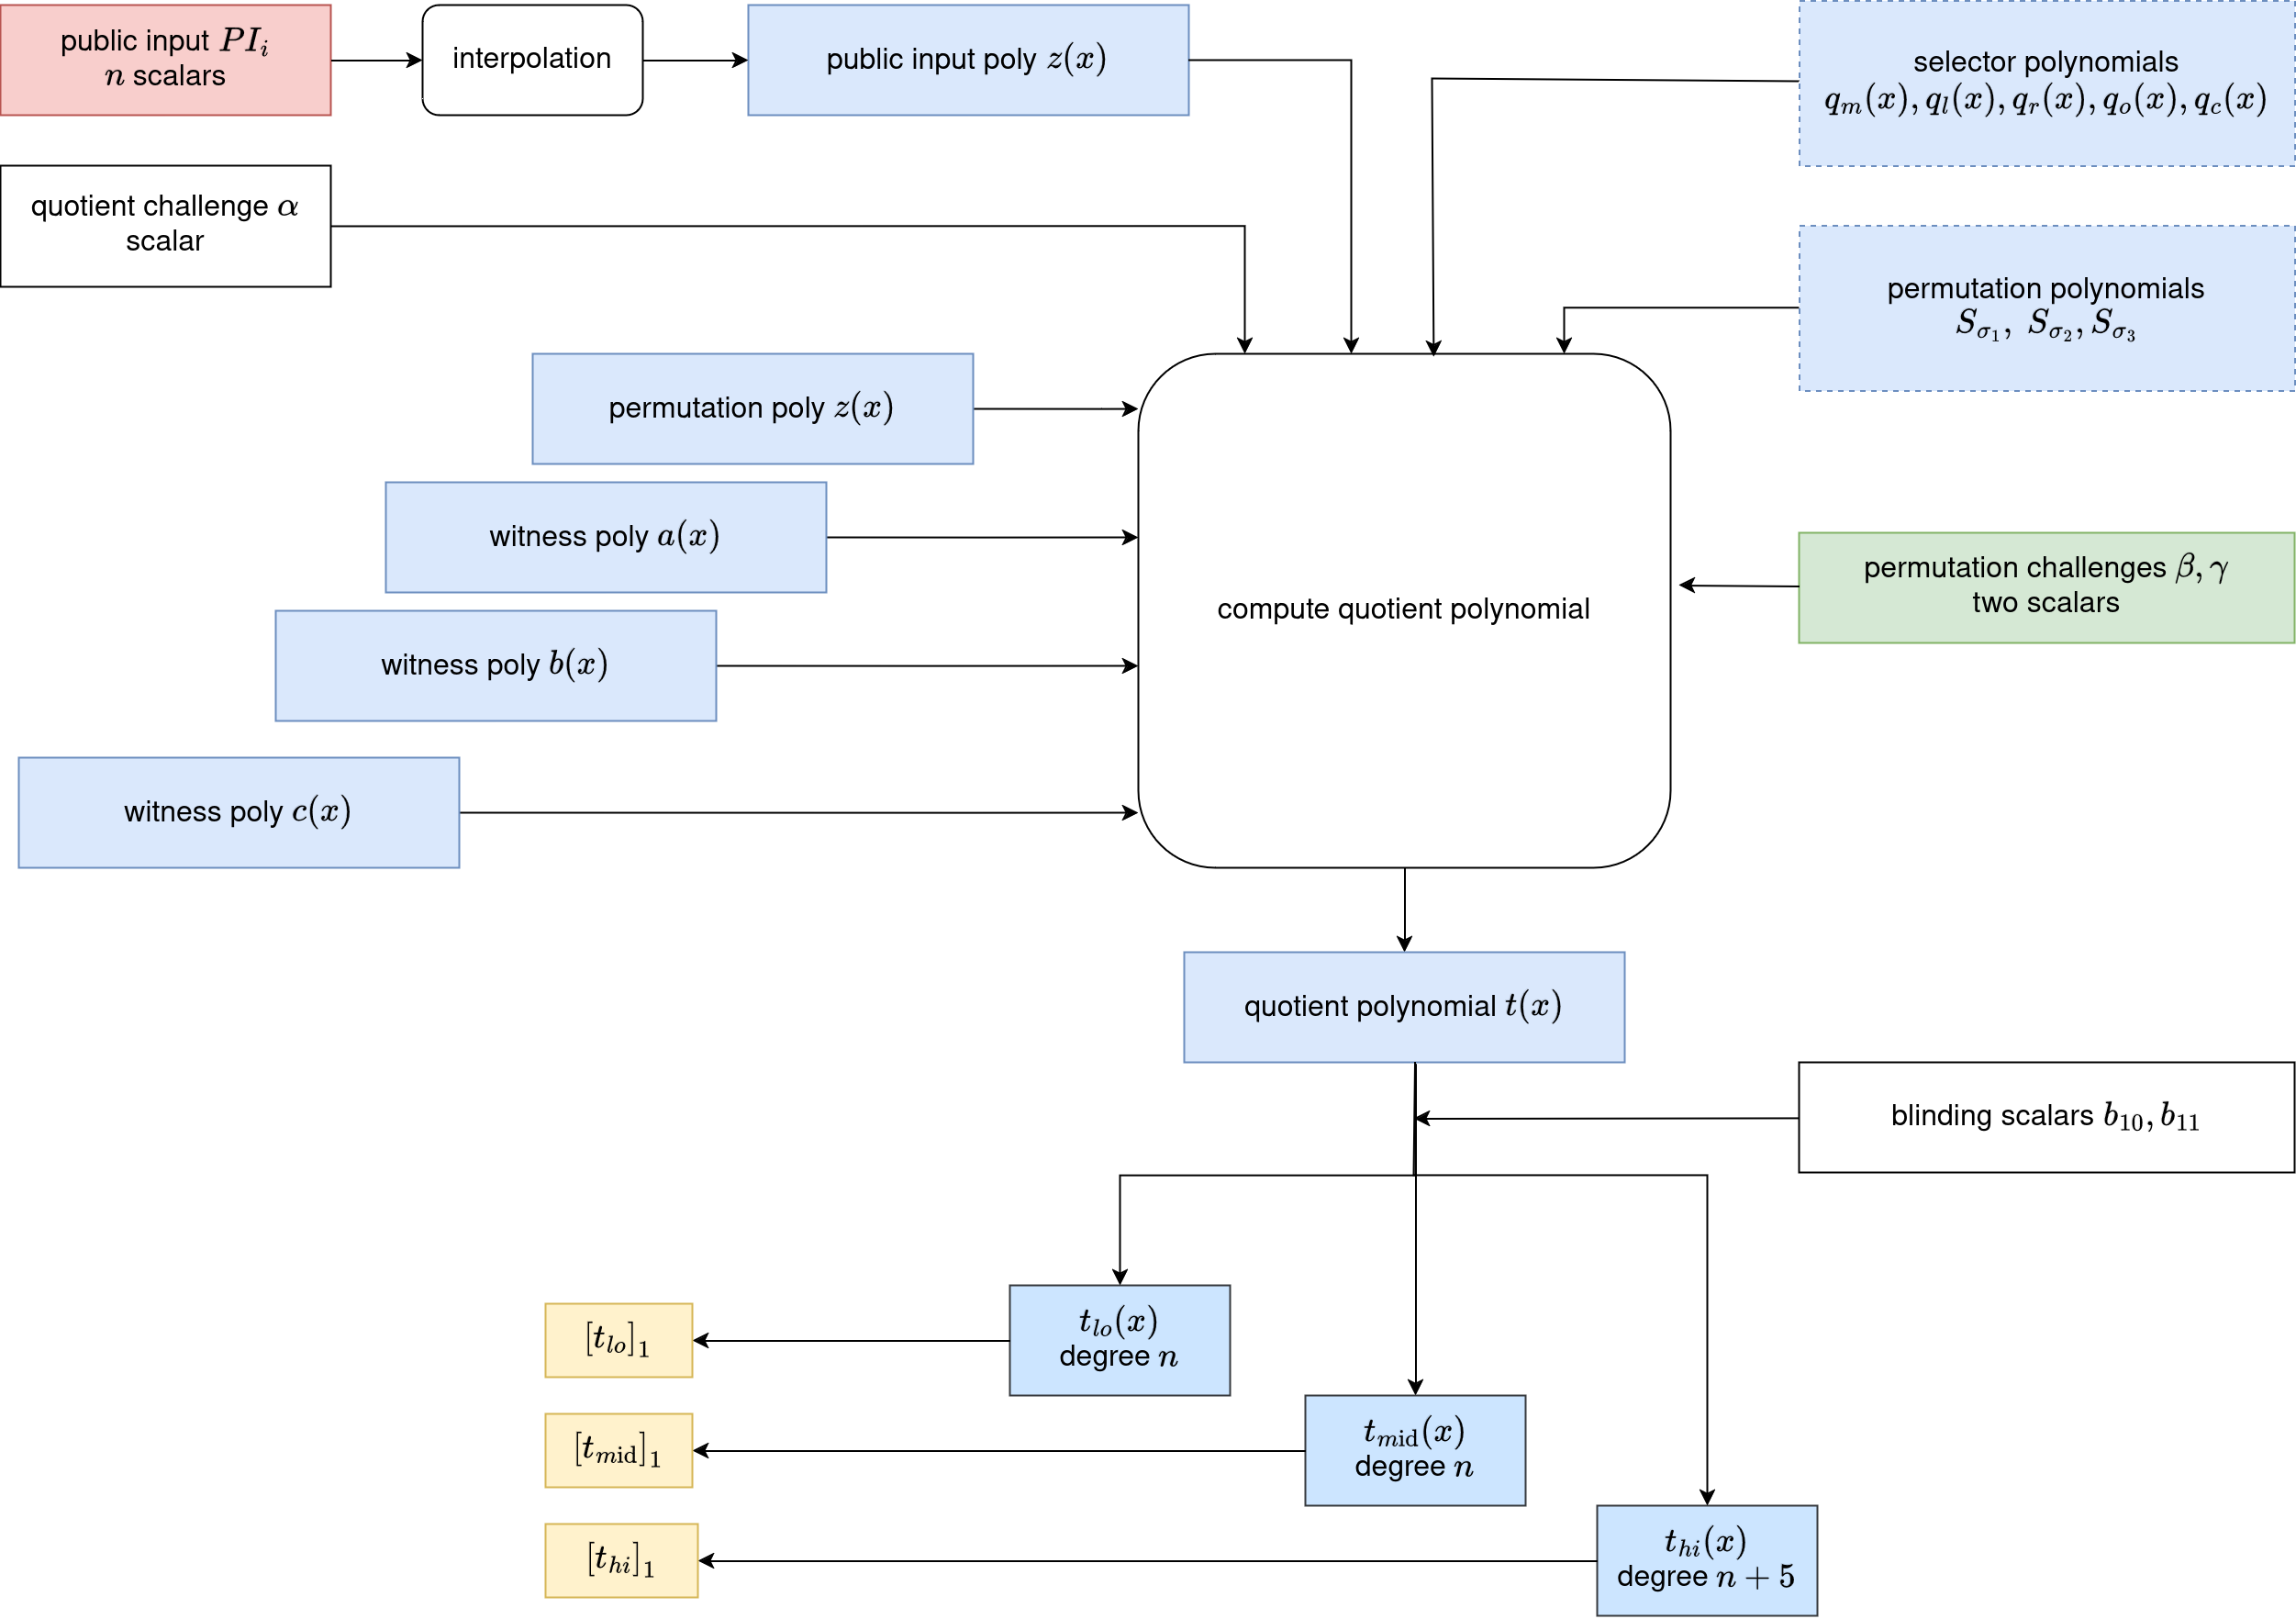
\includegraphics[width=1\linewidth]{round-figures/round3/round3.drawio.png}
    \caption{Enter Caption}    
\end{figure}


In the last round we have computed and committed to $z(x)$ however, we did not prove that it was computed correctly. Specifically we have promised that $z(\omega) = 1$, otherwise for $x = \omega^i$ it is cumulative product $\prod_{j=1}^i f(i) / g(i)$. This is the same as checking:

\begin{enumerate}
    \item $(z(x)-1)L_1(x) = 0$
    \item $z(x)f'(x) = g'(x)z(x\omega)$
\end{enumerate}

$$\Tilde{f}(x) = (a(x) + x \beta + \gamma)(b(x) + x \beta k_1+ \gamma)(c(x) + x \beta k_2+ \gamma)$$
$$\Tilde{g}(x) = (a(x) + \beta S_{\sigma_1}(x) + \gamma)(b(x) + \beta S_{\sigma_2}(x)+ \gamma)(c(x) + \beta S_{\sigma_3}(x) + \gamma)$$

This is not immediately obvious and we will try to show it shortly


In this blog we will not be constructing the quotient polynomial from the bottom. First we will introduce the quotient polynomial in it's full beauty and then dissect it. The quotient polynomial denoted as $t(x)$ in the paper consist of sum of 3 expressions 
$t = t_1 + t_2 + t_3$:
\begin{equation}\label{quotient1}
    t_1(x) = (a(x)q_{l}(x) + b(x)q_{r}(x) + c(x)q_{o}(x) + a(x)b(x)q_{m}(x) + PI(x) + q_{c_i})\frac{1}{Z_H(x)}
\end{equation}

\begin{equation}\label{quotient2}
    t_2(x) = (f'(x)z(x))\frac{\alpha}{Z_H(X)} - (g'(x)z(\omega x))\frac{1}{Z_H(x)}
\end{equation}

\begin{equation}\label{quotient3}
    t_3(x) = (z(x)-1)L_1(x\frac{1}{Z_H(x)}
\end{equation}

$$t(x) = t_1(x) + t_2(x) \alpha + t_3(x) \alpha^2$$

The quotient polynomial might be long but it is composed of elements that pretty much make sense. So let's just work through it.

\subsection{Computing quotient polynomial}

\subsubsection{3rd term}
This corresponds to checking the first part of definition of $z(x)$. So let's prove it is correct: 
\begin{theorem}[First property of permutation polynomial]
    $\forall x \in H: (z(x)-1)L_1(x) = 0 \implies z(\omega) = 1$
\end{theorem}

\begin{proof}
    For $x \neq \omega$ the Lagrange basis evaluate to 0 and there is not any constraint for $z(x)$. However for $x = \omega$ we get $z(\omega) - 1 = 0$ meaning that $z(\omega)$ indeed must be equal to 1.
\end{proof}

\subsubsection{2nd term}
\begin{theorem}[First property of permutation polynomial]
    $\forall i \in [n]: z(\omega^i)f'(\omega^i) = g'(\omega^i)z(\omega^{i+1}) \implies \forall i \in [n]: z(\omega^i) = \prod_{j=1}^{i-1} \frac{f'(\omega^j)}{g'(\omega^j)}$
\end{theorem}

\begin{proof}
    We will show this by induction. For the base case $i=1$ we get:
    $$z(\omega)f(\omega) = g(\omega)z(\omega^2)$$
    $$z(\omega^2) = \frac{f(\omega)}{g(\omega)}$$
    We know that $z(\omega) = 1$ there is already check for that, the rest simplifies easily. For the case $i =k+1$
    $$z(\omega^{k+1})f(\omega^{k+1}) = g(\omega^{k+1})z(\omega^{k+2})$$
    $$\prod_{j=1}^k \frac{f(\omega^j)}{g(\omega^j)} f(\omega^{k+1}) = g(\omega^{k+1})z(\omega^{k+2})$$
    $$\prod_{j=1}^k \frac{f(\omega^j)}{g(\omega^j)} \frac{f(\omega^{k+1})}{g(\omega^{k+1})} = z(\omega^{k+2})$$
    $$z(\omega^{k+2}) = \prod_{j=1}^{k+1} \frac{f(\omega^j)}{g(\omega^j)}$$    
\end{proof}


\subsubsection{1st term}
This might feel familiar and in fact it very much should. These are the gate constraints introduced in the overview \eqref{chap:arithmetization}. Including them in the quotient polynomial makes sure that they indeed hold for each gate. 

Each of the check pass if the designated polynomial is zero on the evaluation domain. We would like to combine like to batch these checks such that $t(x) = 0 \iff t_1(x) = 0 \wedge t_2(x) = 0 \wedge t_3(x) = 0$. To achieve this we will construct the quotient polynomial as:
$$t(x) = t_1(x) + t_2(x)\alpha + t_3(x)\alpha^2$$

Why does this work? The set $\forall \alpha \in \field \{1, \alpha, \alpha^2\}$ is linearly independent:
$$a + b\alpha + c\alpha^2 = 0 \iff a = b = c = 0 $$

To see this let's first assign $\alpha = 0$ which implies that $a = 0$. Now we are left with $b\alpha + c\alpha^2 = 0$. Now we can pick we make following assignment:
$$\alpha = 1: b + c = 0$$
$$\alpha = 1^{-1}: -b + c = 0$$
$$b+c -b +c = 0$$

Here we get that $c = 0$ which means that $b$ also needs to be 0.


\subsection{Splitting quotient polynomial}

Now we can finally construct the quotient polynomial $t(x)$. However, the problem is that the degree of the polynomial is too big. We want our polynomials to have the maximum degree of $n$ to be able to commit to them. We assumed so in the setup while creating SRS and the whole KZG commitment scheme relies on it. We can split $t(x)$ into $< n$ degree polynomials $t_{lo}'(x), t_{mid}'(x)$ and $t_{hi}'(x)$ of degree at most $n+5$ such that: $$t(x) = t_{lo}'(x) + x^nt_{mid}'(x) + x^{2n}t_{hi}'(x)$$

Why $t_{hi}$ has degree bound $n+5$? Look just at $t_2$ where we multiply $\Tilde{f}(x)z(x)$. The degree of $\Tilde{f}(x)$ is $3(n+1)$ because of each of $a(x), b(x), c(x)$ have degree of $n+1$ since they interpolate $n$ points. The permutation polynomial has degree $n+2$ which makes it $4n+5$ and then division by $Z_H$ with degree $n$ resulting in $3n+5$.


How can we split the quotient polynomial? We simply compute the quotient polynomial and take $c_0 + c_1x + c_2x^2 + ... + c_n x^n $ as polynomial $t_{lo}$. Then take $c_{n+1}x^{n+1} + c_{n+2}x^{n+2} + ... + c_{2n}x^{2n}$ divide it by $x^n$ and create $t_{mid}$ with degree $n$. Then we do a similar thing for $t_{hi}$ but divide it by $x^{2n}$.
$$t(x) = t_{lo}(x) + x^n t_{mid}(x) + x^{2n}t_{hi}(x)$$

Nice this looks better, but we also need to blind them. $b_{10}, b_{11} \in \field$ and use them as follows: $t_{lo}(x) = t_{lo}'(x) + b_{10}x^n , t_{mid}(x) = t_{mid}'(x) - b_{10} + b_{11}x^n, t_{hi}(x) = t_{hi}'(x) - b_{11}$. Now we are ready to calculate commitments with degree at most $n+5$: $[t_{lo}(s)]_1, [t_{mid}(s)]_1, [t_{hi}(s)]_1$.

\procedureblock[linenumbering]{$Round3_{\prover}$}{
    \alpha \sample \field \\
    t(x) =  t_1(x) + t_2(x) \alpha + t_3(x) \alpha^2 \\
    t(x) -> t_{lo}, t_{mid}, t_{high} \\
    \pcreturn [t_{lo}]_1, [t_{mid}]_1, [t_{high}]_1 \\
}

% ==============================================================================
% ===ROUND4=====================================================================
% ==============================================================================
\section{Round 4}
\label{chap:round4}

\begin{enumerate}
    \item Compute evaluation challenge $\challenge \in \field = \challenge$
    \item Compute and output opening evaluations $\overline{a}, \overline{b}, \overline{c}, \overline{z_\omega}, \overline{S}_{\sigma_1}, \overline{S}_{\sigma_2}$
\end{enumerate}

\begin{figure}[H]
    \centering
    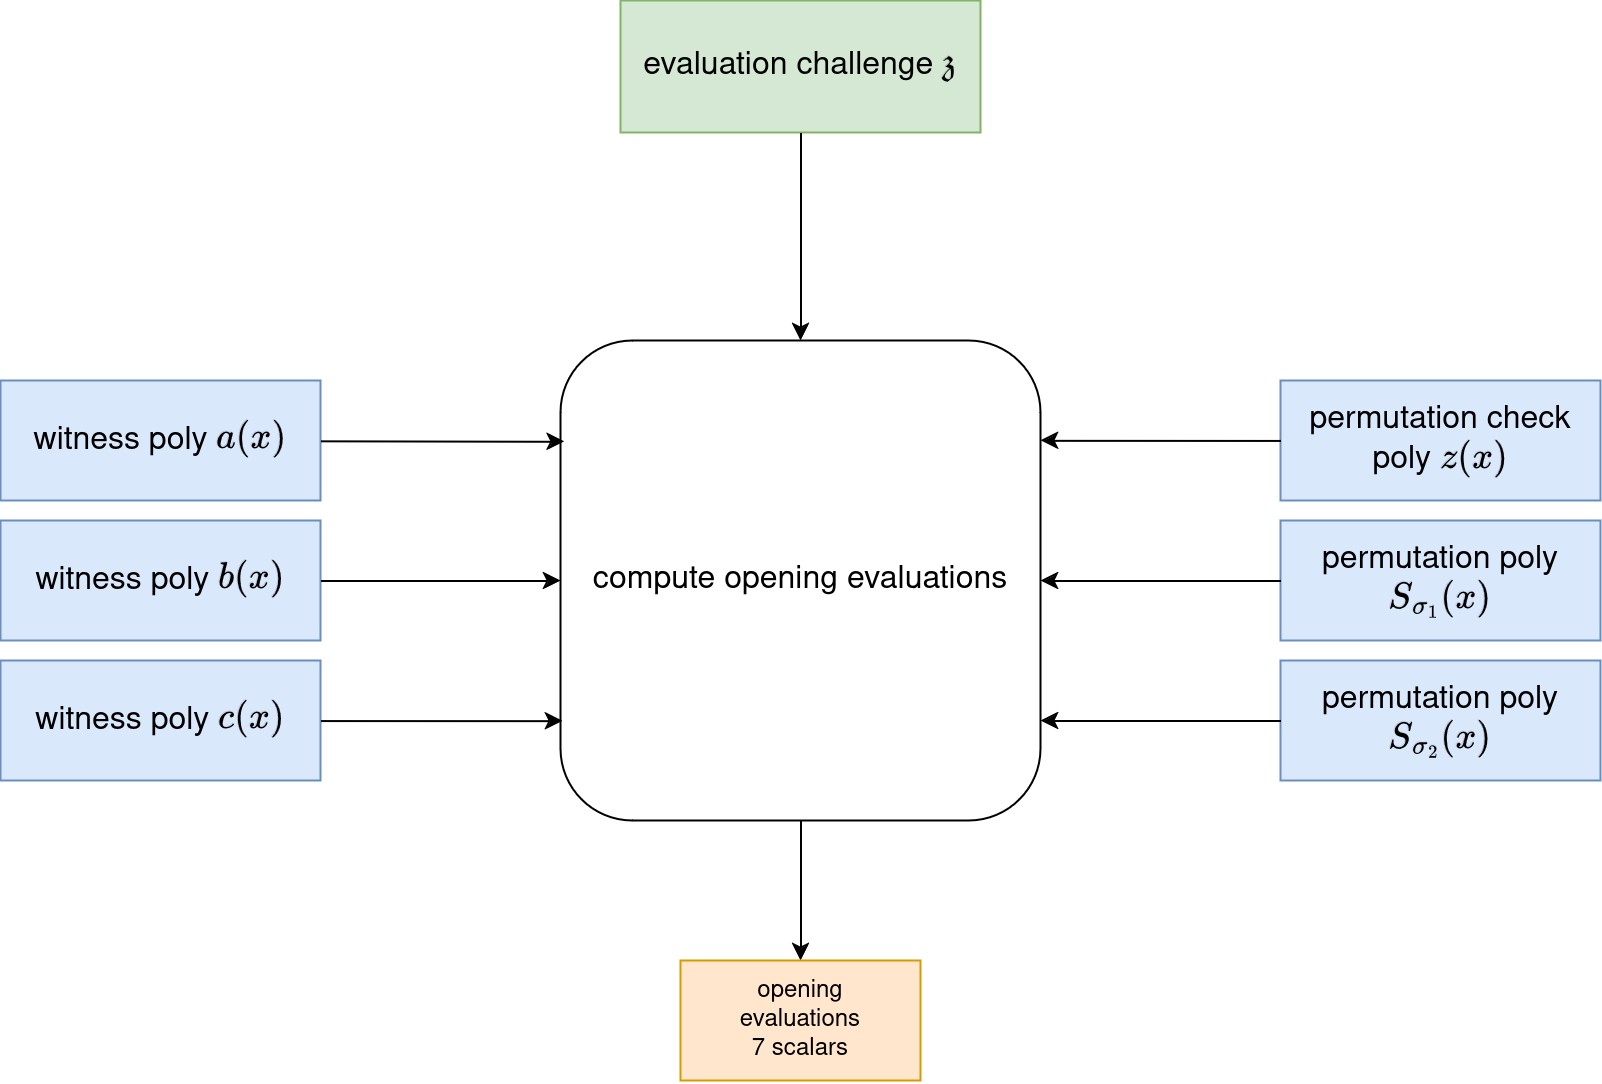
\includegraphics[width=1\linewidth]{round-figures/round4/round4.drawio.png}
    \caption{Enter Caption}
    
\end{figure}

In this round the prover computes evaluation opening, know in the business as linearisations, which are denoted with a horizontal line above. The openings are performed at a random point $\challenge$. In interactive case $\challenge$ is chosen by the verifier, here it is given by a hash function applied to transcript of the prover computation. All the prover has to do is calculate and output: $\overline{a} = a(\challenge), \overline{b} = b(\challenge), \overline{c} = c(\challenge), \overline{z_\omega} = z(\omega\challenge),\overline{S}_{\sigma_1} = S_{\sigma_1}(\challenge), \overline{S}_{\sigma_2} = S_{\sigma_2}(\challenge)$. Is is as simple as that. Now let's look at a way to minimize number of opening to minimize protocol communication costs.

\subsection{Linearization trick}
Imagine that the prover wants to show that $h_1(x)h_2(x) - h_3(c) = 0$ over a specified domain. Then he sure needs to commit to each to these polynomials and send their openings at a random point $\challenge$, resulting in 3 commitments and 3 openings. Verifier needs to check $\forall x \in H: h_1(x)h_2(x) - h_3(c) = 0$ which thanks to \href{https://en.wikipedia.org/wiki/Schwartz%E2%80%93Zippel_lemma}{Schwartz-Zippel} simplifies to checking just at a single random point $\challenge$. 

There is a better approach, utilizing the linearisation polynomial $l(x) = \overline{h}_1 h_2(x) - h_3(x)$ which as usual evaluates to zero over the domain $H$. As before the prover needs to send commitments $[h_1]_1, [h_2]_1, [h_3]_1$. However now he will send only 2 openings of $\overline{h_1} = h_1(\challenge)$ and $\overline{l} = l(\challenge) = \overline{h_1}h_2(\challenge) - h_3(\challenge)$. Notice that the number of the commitments stays the same because the verifier can calculate $[l]_1 = \overline{h}_1[h_2]_1 + [h_3]_1$. This is possible because commitments are additively homomorphic. The verifier checks that $l(\challenge) = 0$ which is equivalent to $h_1(\challenge)h_2(\challenge) - h_3(\challenge) = 0$ from how we defined $l(x)$. Keep in mind there is not anything complex, you can see the difference in the comparison below. The left diagram has 3 opening and the right one is the modified one with 2 opening and the linearisation polynomial.

\begin{figure}[H]
    \centering
    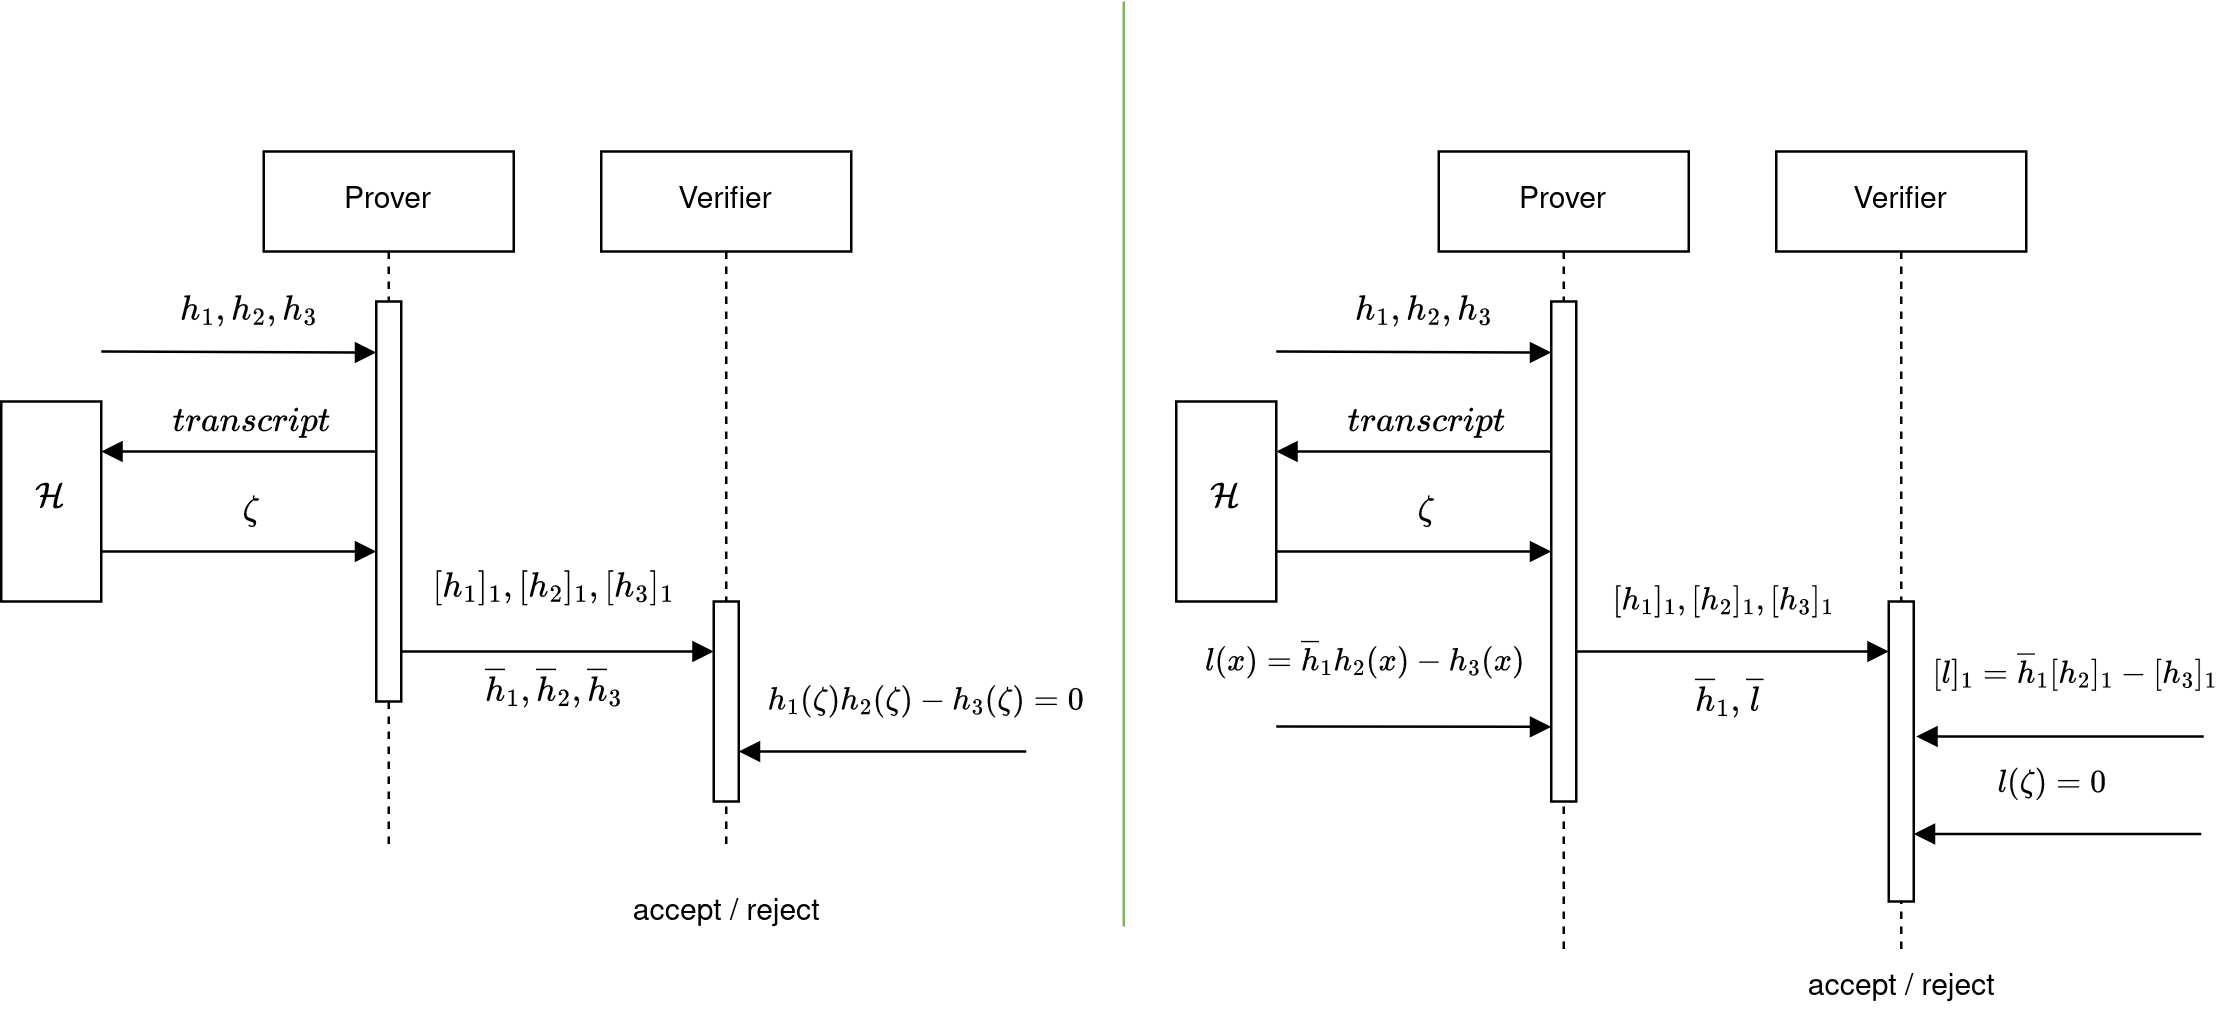
\includegraphics[width=1\linewidth]{round-figures/round4/linearisation_trick.drawio.png}
    \caption{Linearization trick}
\end{figure}

Why do we need to send $\overline{h}_1$?
Elliptic curve pairing which are not homomorphic for multiplication, meaning we cannot multiply to commitments so it is not possible to compute commitment to $l$ as $[l]_1 = [h_1]_1[h_2]_1 - [h_3]_1$. By sending $\overline{h}_1$ we can calculate the multiplication $\overline{h}_1[h_2]_1$ since here we perform multiplication by opening which is effectively a constant.

The linearisation trick is the reason why we are not sending evaluation at $\challenge$ for selector polynomials $q_l(x), q_r(x), q_m(x), q_c(x)$, permutation function $S_{\sigma_3}$ and permutation $z(x\omega)$ in the following round. That already is a significant improvement. If you are asking why do we need $z(x\omega)$ it is to check for 2. part of definition for the permutation polynomial $z(x)$.

\procedureblock[linenumbering]{$Round4_{\prover}$}{
    \challenge \\
    \overline{a} = a(\challenge), \overline{b} = b(\challenge), \overline{c} = c(\challenge), \overline{z_\omega} = z_\omega(x), \overline{S}_{\sigma_1} = S_{\sigma_1}(x), \overline{S}_{\sigma_2} = S_{\sigma_2}(x) \\
    \pcreturn \overline{z_\omega}, \overline{S}_{\sigma_1}, \overline{S}_{\sigma_2}
}

% ==============================================================================
% ===ROUND5=====================================================================
% ==============================================================================
\section{Round 5}
\label{chap:round5}

Previously we have seen how to perform linearisation trick to minimize the number of openings. We will use this knowledge in the grand finale of the prover algorithm. Here all of the constraints will be combined to generate the proof $\pi$ which will be sent to the verifier.

\begin{enumerate}
    \item Compute opening challenge $v \in \field$
    \item Compute linearisation polynomial $r(x)$
    \item Compute opening proof polynomial $W_{\challenge}(x)$
    \item Compute opening proof polynomial $W_{\challenge\omega}(x)$
    \item Return proof $\pi$
\end{enumerate}

\begin{figure}[H]
    \centering
    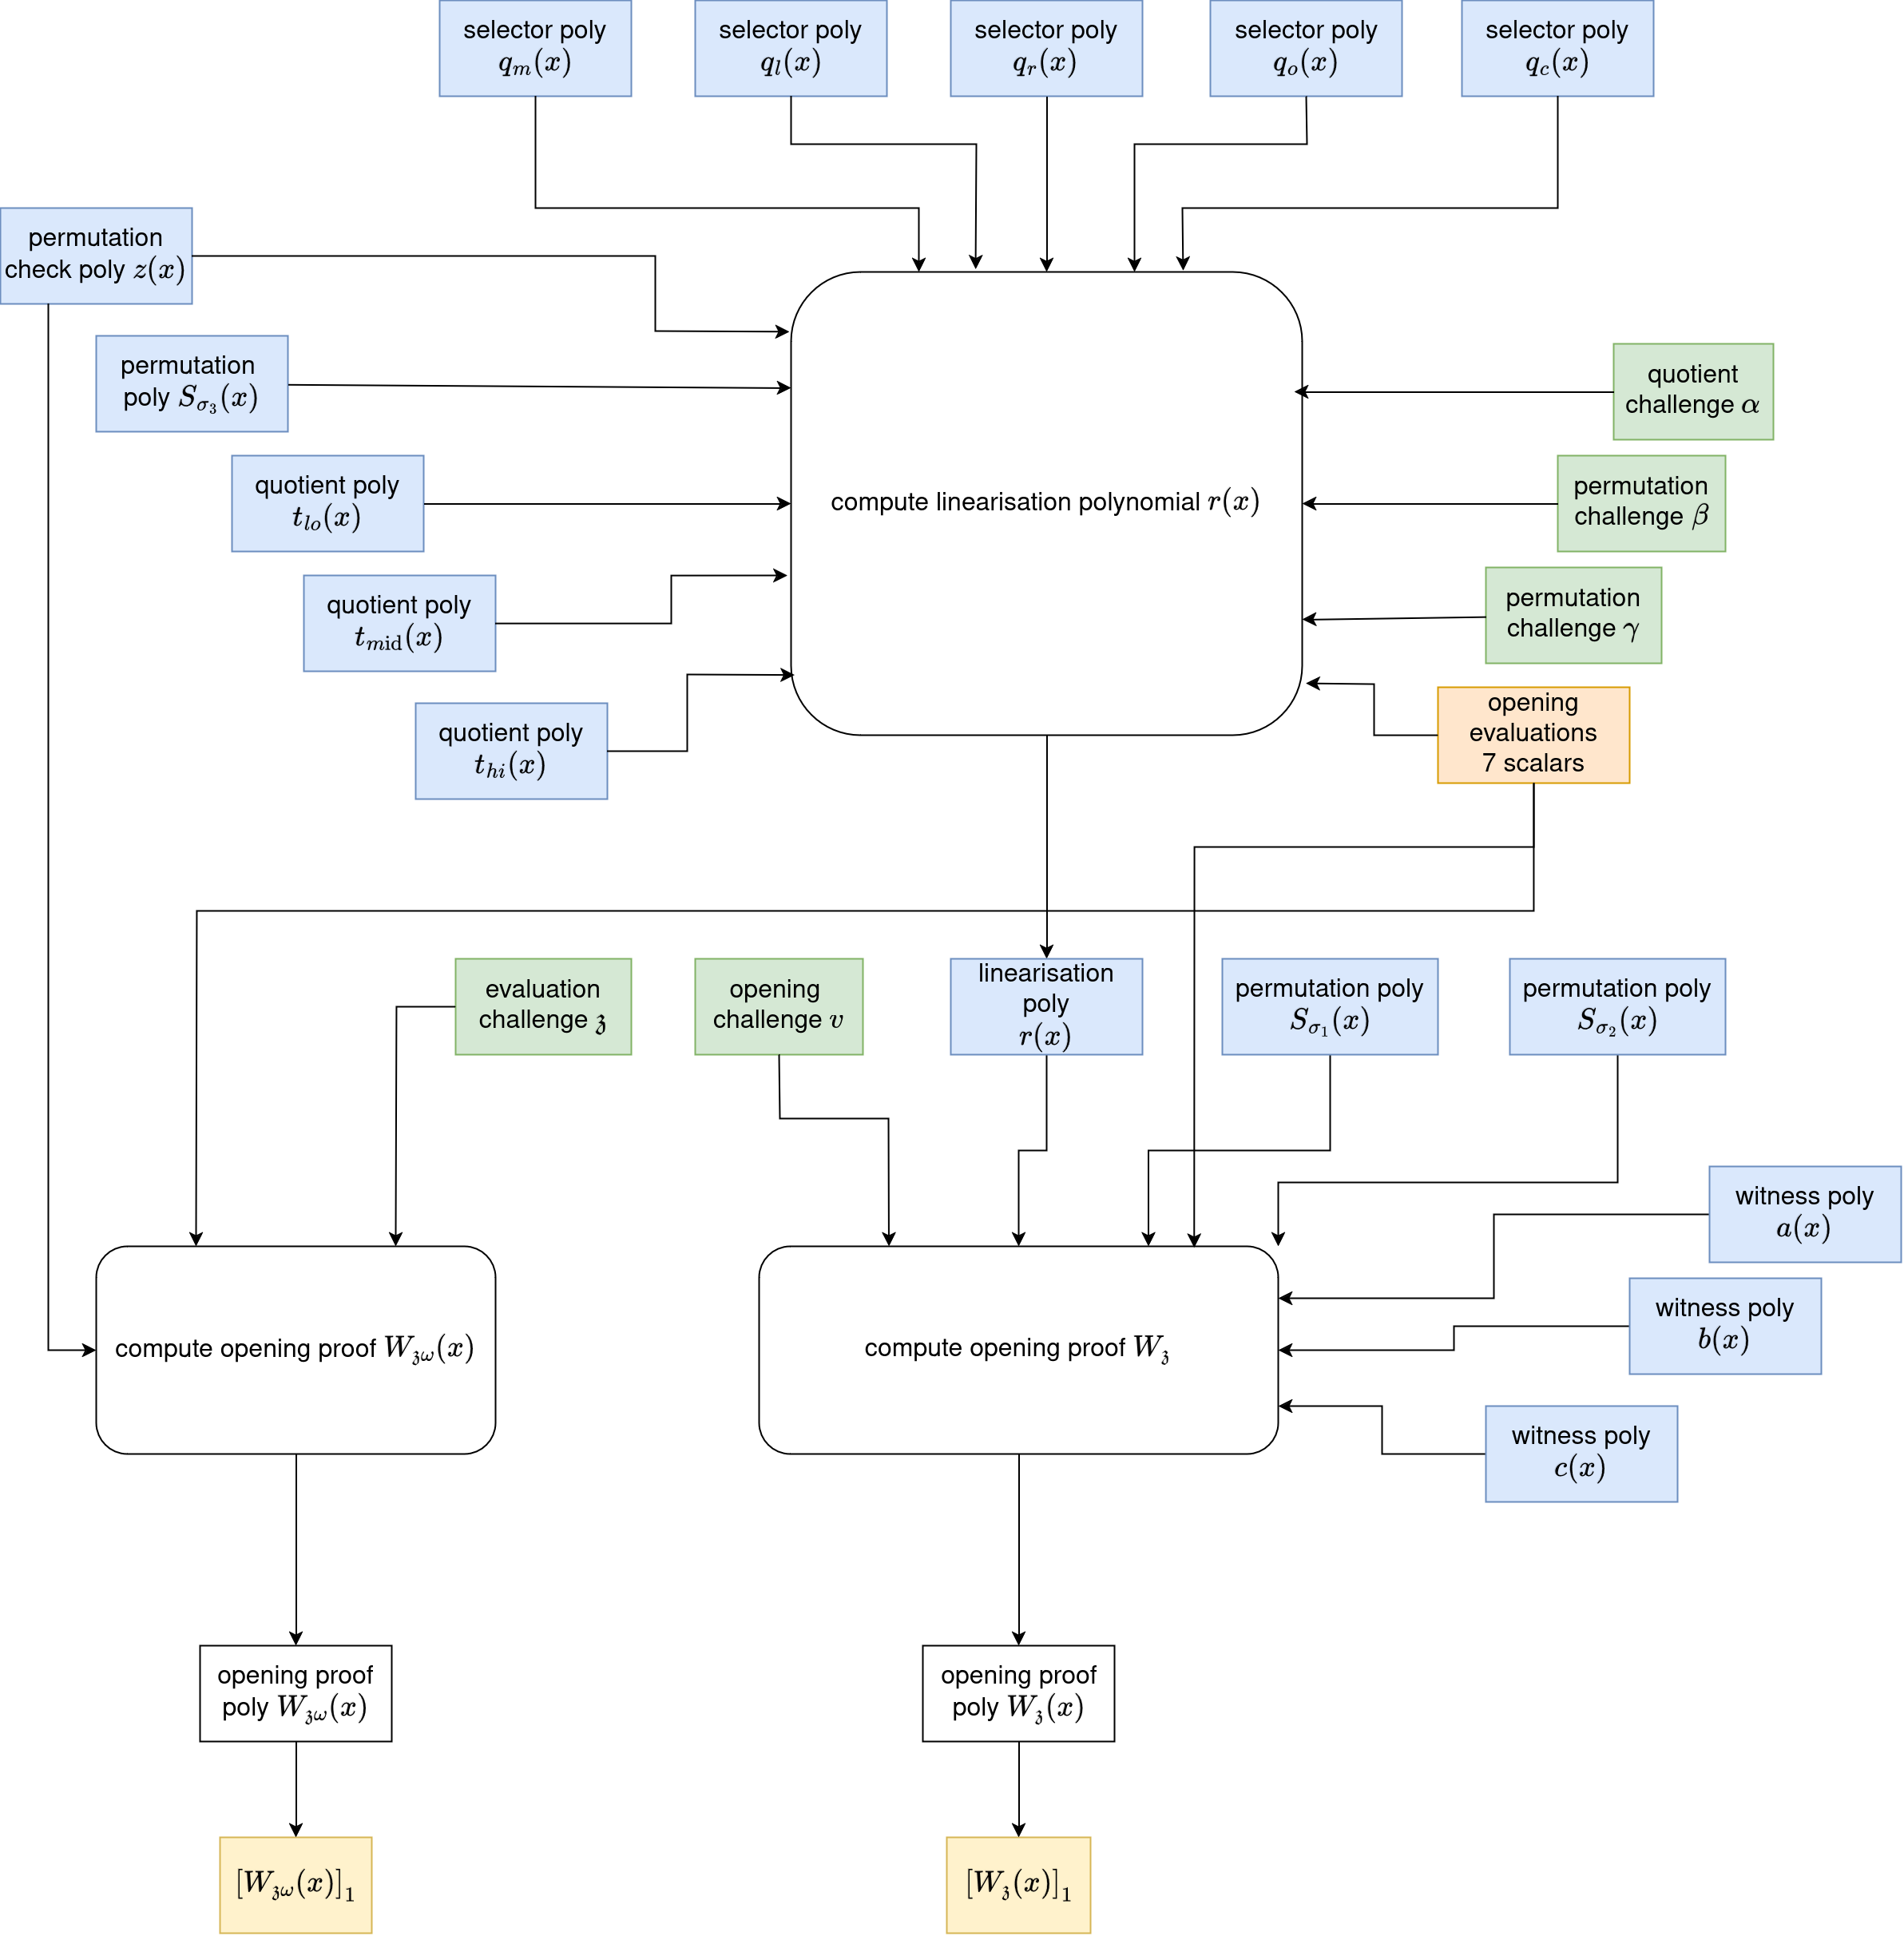
\includegraphics[width=1\linewidth]{round-figures/round5/round5.drawio.png}
    \caption{Enter Caption}
    
\end{figure}

\subsection{Linearisation polynomial}
Prover computes linearisation polynomial $r(x)$ which is a linear combination of all commitments. This polynomial is created using the evaluations from the round 4. Recall from the third round: 
\begin{equation}\label{pseudo-linearisation-poly}
    t_{lo} + x^{n}t_{mid}(x) + x^{2n}t_{hi} = t(x) = \frac{s(x)}{Z_H(x)}
\end{equation}

We know that the quotient polynomial should evaluate to zero over the domain $H$, therefore needs to exists a polynomial $s$ for which above holds. From that we can construct the linearisation polynomial:
$$r(x) = s(x) - Z_H(\challenge)(t_{lo}(x) + \challenge^n t_{mid}(x) + \challenge^{2n}t_{hi}(x)$$

Notice that this polynomial is just rewritten \eqref{pseudo-linearisation-poly} from which follows that it should be zero when evaluated at the point $\challenge$. In the full form the quotient polynomial could be written as:

\begin{multline}
    r(x) = [\overline{a}\overline{b}q_m(x) + \overline{a}q_l(x) + \overline{b}q_r(x) + \overline{c}q_o(x) + PI(\challenge) + q_c(x)] \\
    + \alpha [
        (\overline{a} + \beta \challenge + \gamma)(\overline{b} + \beta k_1 \challenge + \gamma)(\overline{c} + \beta k_2 \challenge + \gamma)z(x) \\
        - (\overline{a} + \beta \overline{s}_{\sigma_1} + \gamma)(\overline{b} + \beta \overline{s}_{\sigma_2} + \gamma)(\overline{c} + \beta S_{\sigma_3}(x) + \gamma)\overline{z}_{\omega}
    ] \\
    + \alpha^2 [(z(x) -1)L_1(\challenge)] \\
    - Z_H(\challenge)(t_{lo}(x) + \challenge^n t_{mid}(x) + \challenge^{2n} t_{hi}(x))
\end{multline}

Here the polynomial $s$ is substituted by the \textit{gate check} + \textit{1. permutation check} + \textit{2. permutation check}. It is good to notice which variables are linearised. They are the ones without the horizontal line: $q_m, q_l, q_r, q_o, q_c, z, S_{\sigma_3}$. This is determined by the linearization trick described in the previous post \eqref{chap:round4}. After you understand why those could be linearized and others not make sure to understand that the prover is able to calculate the commitment to $r(x)$ from the proof $\pi$ at the end of this post. 

\subsection{Opening proof polynomial}

\subsubsection{First opening proof polynomial}
Prover calculates $W_{\challenge}(x)$ the opening proof polynomial to verify that linearisation polynomial $r(x) = 0$ over $H$, by opening a single evaluation $\challenge$. This a form of aggregation and is essentially the same as checking that each of the constraints obtained in $r(x)$ evaluate to 0. Besides the verifier also needs to check for correctness of $a(x), b(x), c(x), S_{\sigma_1}(x), S_{\sigma_2}(x)$. These are combined into linearly independent set using $(1, v, v^2, v^3, v^4, v^5)$ where $v \in \field$ is given from $\mathcal{H}(transcript)$. Linear independence is used for similar reason as in the quotient polynomial.

\begin{multline}
    W_{\challenge}(x) = \frac{1}{x - \challenge} (
        r(x) 
        + v(a(x) - \overline{a})) 
        + v^2(b(x) - \overline{b})) \\
        + v^3(c(x) - \overline{c})) 
        + v^4(S_{\sigma_1}(x) - \overline{S}_{\sigma_1})) 
        + v^5(S_{\sigma_2}(x) - \overline{S}_{\sigma_2})) 
\end{multline}

The prover needs to show that all of the terms are divisible by $x - \challenge$ meaning that $\challenge$ is a root for each of them.

Let's be a bit more specific about previous check
If $x - \challenge$ divides a polynomial, in our case $r(x)$, that means there needs to exist $s(x)$:
$$\frac{r(x)}{z-\challenge} = s(x)$$
$$r(x)= s(x)(x-\challenge)$$
That means $r$ has $\challenge$ as root. The rest of the polynomials are in the form: $(p(x) - \overline{p})$. The check essentially says: if $x - \challenge$ divides $p(x) - \overline{p}$ then $p(\zeta) = \overline{p}$ meaning the polynomial was linearised correctly.
$$\frac{p(x) - \overline{p}}{x-\challenge} = s(x)$$
$$p(x) - \overline{p}= s(x)(x-\challenge)$$

If evaluated at $\challenge$ we would indeed get $\overline{p} = p(\challenge)$


\subsubsection{Second opening proof polynomial}
Prover calculates $W_{\challenge\omega}(x)$. Recall that in the quotient polynomial $t(x)$ both $z(x), z(z\omega)$ appear. Thanks to the linearization trick in \eqref{chap:round4} it is sufficient to compute $\overline{z_\omega}$. The evaluation $\overline{z}$ is not needed and commitment to $r(x)$ can be computed without it. However as $z(x)$ is opened at $\challenge\omega$ instead of $\challenge$ we need a separated opening polynomial $W_{\challenge\omega}(x)$, which is the final polynomial that the prover needs to calculate.

$$W_{\challenge\omega}(x) = \frac{z(x)-\overline{z}_{\omega}}{x - \challenge\omega}$$

This polynomial checks that $z(\challenge\omega) = \overline{z}_\omega$ in the same way as described for the opening polynomial $W_{\challenge}(x)$.



\section{Return Proof}
Now the prover can finally send the whole proof:
$$\pi = ([a]_1, [b]_1, [c]_1, [z]_1, [t_{lo}]_1, [t_{mid}]_1, [t_{hi}]_1, [W_{\challenge}]_1, [W_{\omega\challenge}]_1, \overline{a}, \overline{b}, \overline{c}, \overline{z_\omega}, \overline{S}_{\sigma_1}, \overline{S}_{\sigma_2})$$





\chapter{Security and Efficiency}
\label{chap:4}

The role of the prover is to convince the verifier about the valid execution of a specified arithmetic circuit by showing that conditions form \Cref{sec:checks} are satisfied. This is done by constructing specific polynomials and proving their evaluation at uniformly randomly selected points using the KZG polynomial commitment scheme. It might not be directly clear from the diagram \Cref{fig:full-diagram}, but the whole protocol is basically a batched KZG for polynomials that prove valid execution of the circuit.

\begin{figure}
    \centering
    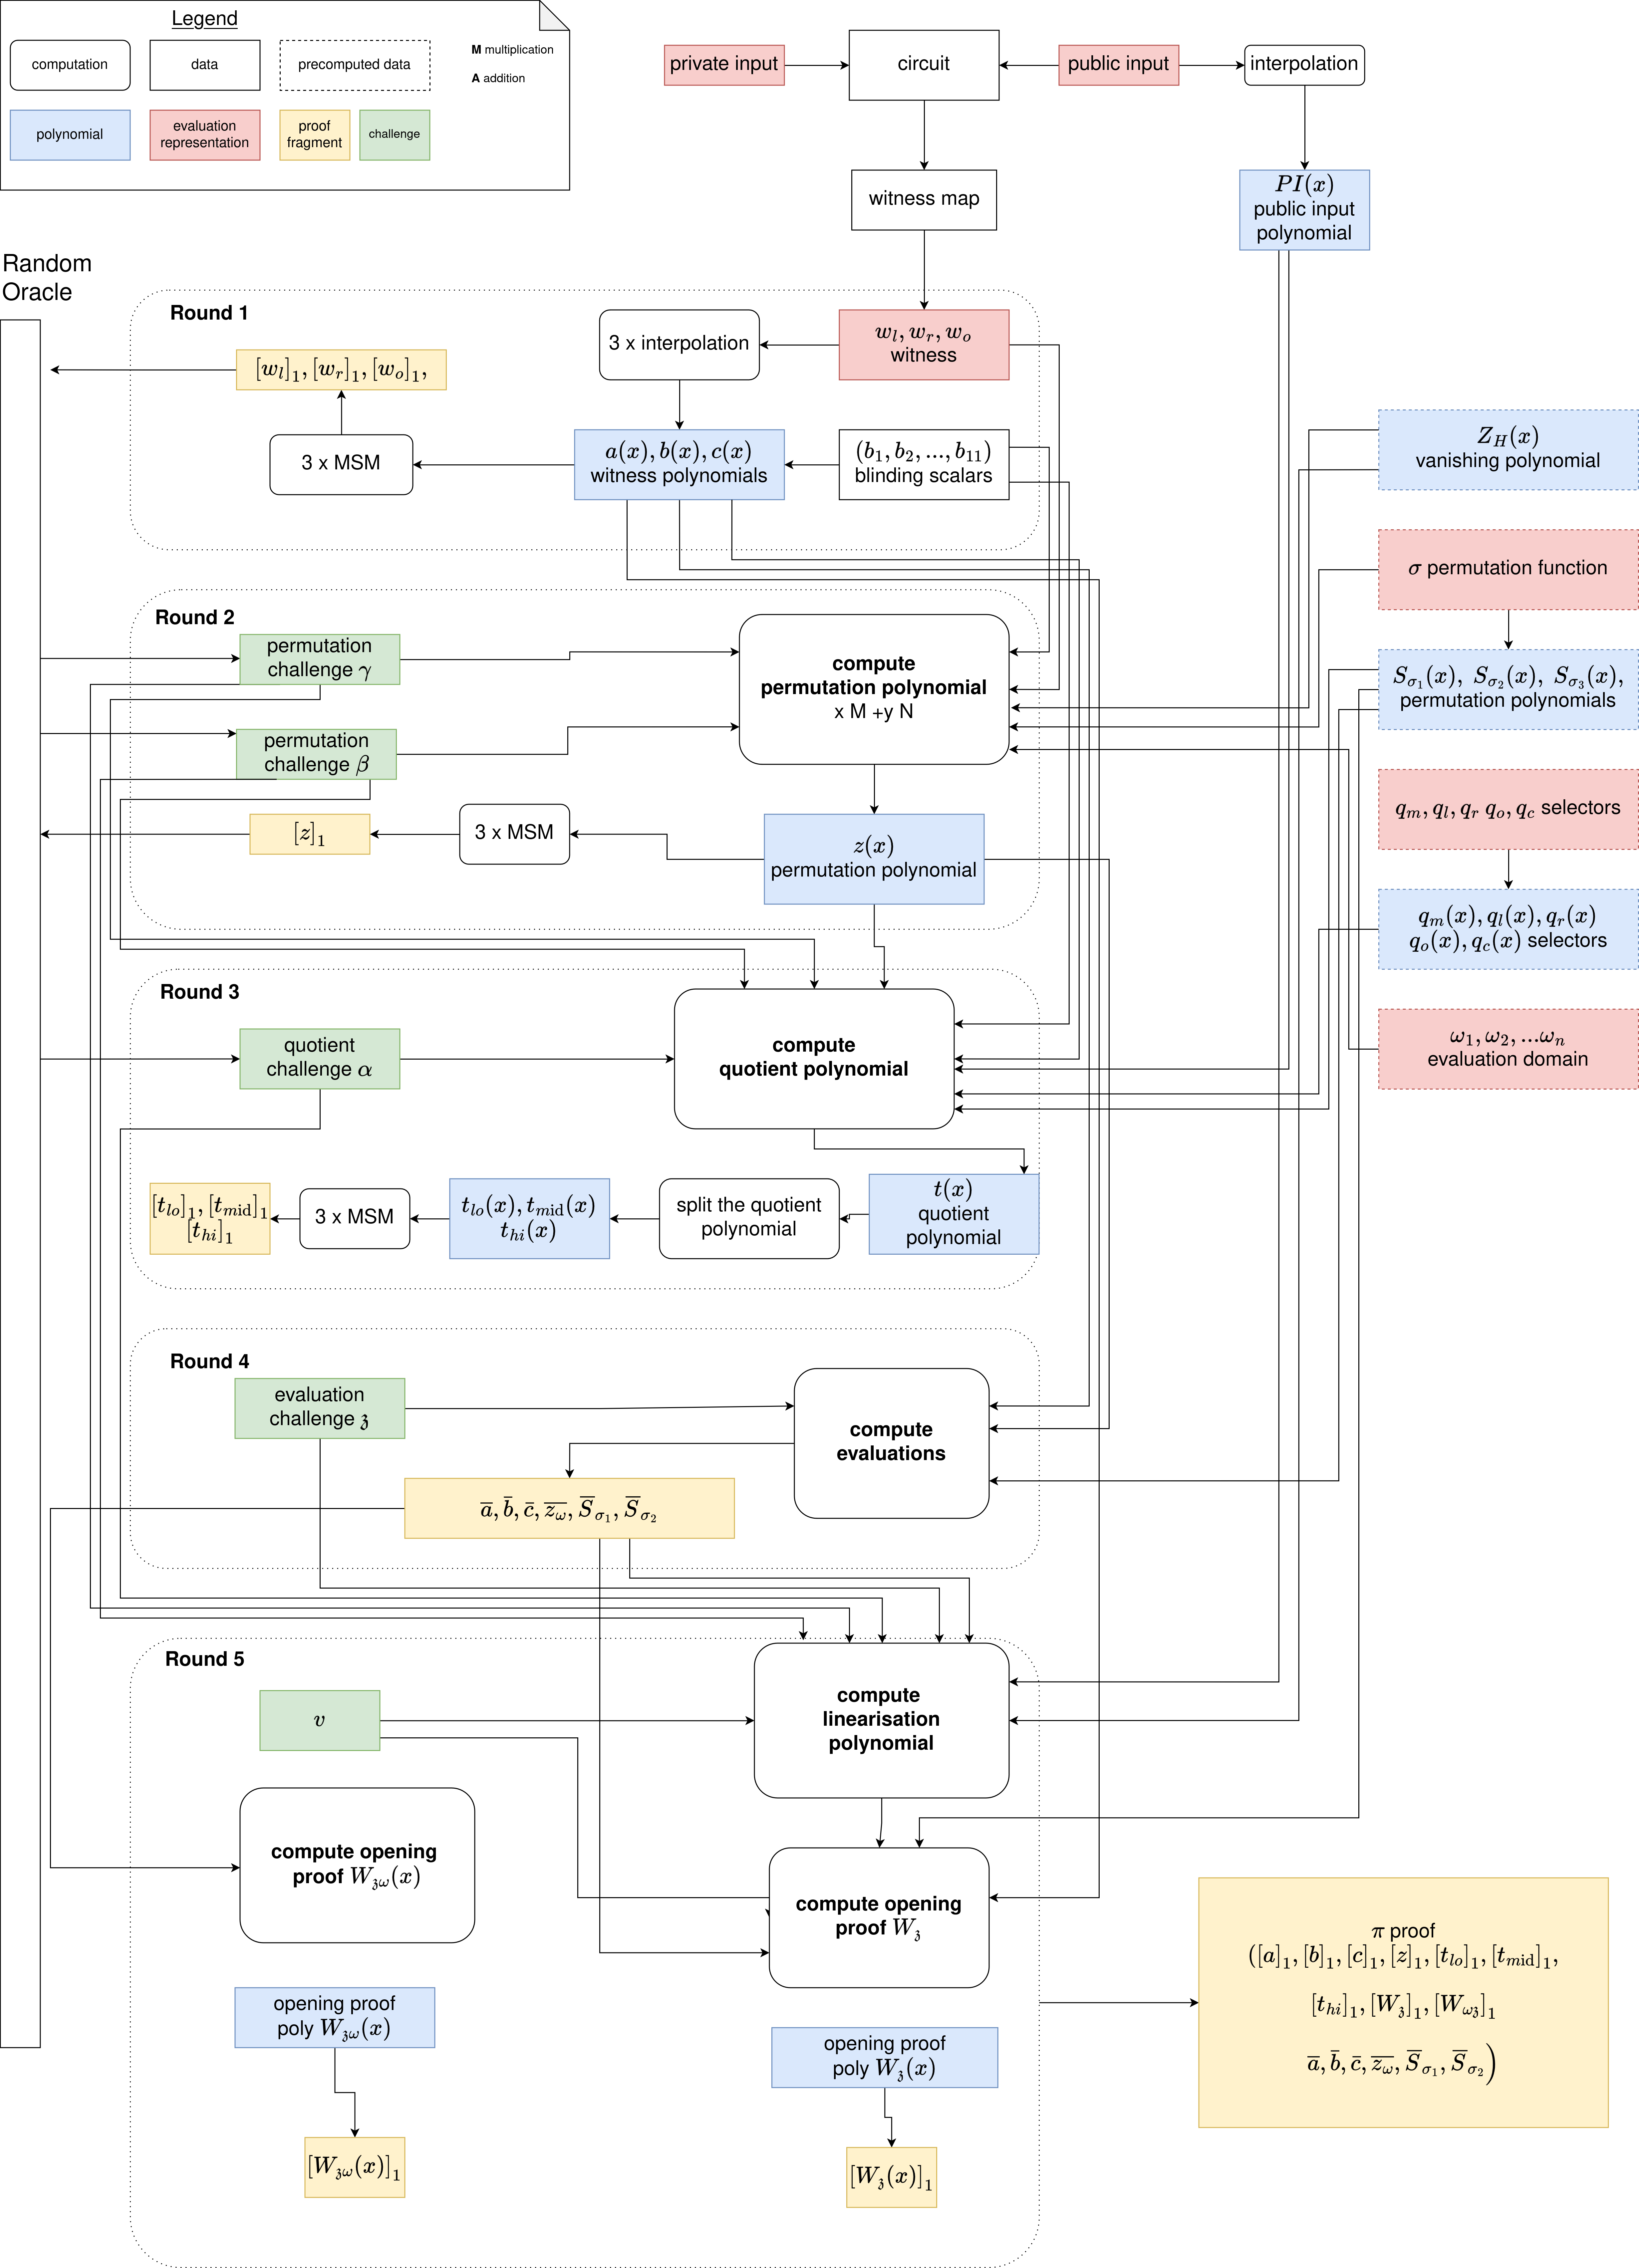
\includegraphics[width=1\linewidth]{round-figures/prover-algorithm.drawio.png}
    \caption{Diagram of prover algorithm}
    \label{fig:full-diagram}
\end{figure}

Degree bound on the polynomials constructed by the prover:
\begin{itemize}
    \item Wire polynomials $deg(a(x)) = deg(b(x)) = deg(c(x)) = n+1$ determined the multiplication of blinding polynomial of degree 1 and the vanishing polynomial of degree $n$.
    \item Permutation polynomial $deg(z(x)) = n+2$ determined by multiplication of blinding polynomial of degree 2 and vanishing polynomial of degree $n$
    \item Quotient polynomial $deg(t(x)) 3n+5$ described in the round 3 \Cref{sec:polynomial-splitting}
    \item Split quotient polynomials $deg(t_{lo}(x)) = deg(t_{mid}(x)) = n, deg(t_{hi}(x)) = n+5$ quotient polynomial is split into 3 smaller polynomials
    \item Linearisation polynomial $deg(r(x)) = n+5$ as described in round 4 \Cref{chap:round4} the linearisation polynomial cannot contain polynomial multiplication. Therefore, the degree is determined by the polynomial of the highest degree, which is $t_{hi}(x)$
    \item Opening proof polynomial $deg(W_{\challenge}(x)) = n+4$ degree is determined by $t(x)$ and consequently divided by $(x - \challenge)$
    \item Opening proof permutation polynomial $deg(W_{\challenge\omega}(x)) = n+1$ degree is determined by $z(x)$ and divided by $(x - \challenge\omega)$
\end{itemize}

\section{Advantages and limitations}

The plonk protocol can run for a general circuit of some size that is bounded by the $KZG$ setup. The setup, in the form of common preprocessed input, is updatable, and the trusted KZG setup can be reused for any circuit of a given size bound. Moreover, the size of the proof is constant. 

A downside of the protocol is the requirement for a trusted setup. As stated in the article \cite{pipeMSM}, the calculation of the commitments seems to be a major bottleneck of $\plonk$ and other SNARK protocols. Another major bottleneck is FFT. There is a lot of effort to make the prover algorithm more effective. Possible ways for the protocol optimization are mentioned in the \Cref{optimization-possibilities}. 



\section{Properties of the protocol}

\begin{theorem}
    \label{main-theorem}
    The $\plonk$ protocol is a succinct, non-interactive, complete, knowledge-sound, and zero-knowledge.
\end{theorem}

\paragraph{Succinctness:} The proof $\pi$ consists of 9 commitments and 6 openings, so for an arbitrarily large circuit, the proof size remains constant. The verification algorithm must perform sanity checks, evaluate 3 public polynomials, calculate 3 additional commitments, and perform a single batched KZG verification procedure. The number of operations does not change with respect to the size of the circuit, so we can conclude that the protocol is succinct.

\paragraph{Non-Interactivity:} Non-interactivity is achieved by the Fiat-Shamir heuristic, where the prover can effectively generate challenges by accessing a random oracle $\mathcal{H}$. We will not show the correctness of the application of this heuristic.

\paragraph{Completeness:} Correctness of $\plonk$ is dependant on many building blocks. Correctness of the checks for the arithmetic circuit was established by \Cref{input-correctness-soundness}, \Cref{output-correctness-soundness}, \Cref{gate-correctness-soundness}, \Cref{permutation-correctness-soundness}, and we also showed the correctness of the KZG polynomial commitment scheme \Cref{kzg-correctnes}.

\paragraph{Knowledge Soundness:} We showed the soundness of each of the checks for the arithmetic circuit \Cref{input-correctness-soundness}, \Cref{output-correctness-soundness}, \Cref{gate-correctness-soundness}, \Cref{permutation-correctness-soundness}. We did not show the soundness of KZG but referred to \cite{ProofArgsAndZk}.

\paragraph{Zero-Knowledge:} Since the proof contains only commitments and polynomial opening, it is sufficient to show that masking polynomial makes the KZG polynomial commitment scheme zero-knowledge, which was proven in \Cref{theorem:blinding}.

With respect to the above discussion, we can conclude the \Cref{main-theorem} is proven. 


\chapter{Optimizations}
\label{chap:5}

Upon publishing, $\plonk$ became a popular SNARK, and variants of the protocol have been implemented in many cryptocurrency projects. This led to efforts to make the protocol more efficient. The optimizations can be done on three fronts:
\begin{itemize}
    \item Polynomial commitment scheme 
    \item Interactive Protocol
    \item Recursive proof composition
\end{itemize}

\section{Possibilities for optimization}
\label{optimization-possibilities}

\subsection{Polynomial commitment scheme:} The $\plonk$ protocol was initially described with the KZG \cite{KZG} polynomial commitment scheme, but other polynomial commitment schemes like FRI \cite{fri} could be used as well. As mentioned, commitments realized by MSM place a large computational load on the prover. One of the authors of $\plonk$ has already written a follow-up article on the construction of efficient polynomial commitment schemes for multiple points and polynomials \cite{shplonk} that can be used in $\plonk$.

\subsection{Interactive protocol:} This covers the rest of the protocol that is not about the polynomial commitment scheme. The possibilities for optimization range from more effective arithmetization to constructing more efficient polynomial checks. The major work in this area was done on the use of custom gates and the construction of lookup tables. By using more complex custom gates, it is possible to reduce the degree of the circuit, which determines the complexity of the prover. Custom gates are described in detail in \textit{TurboPlonK} \cite{turboplonk}. The lookup tables from \textit{plookup} \cite{plookup} enable to precompute values for inputs $\publicinput$ and then prove that the witness $\witness$ exists in that table. These two approaches are independent and can be combined, as shown in \textit{HyperPlonK} \cite{HyperPlonk}.

\subsection{Recursive proof construction:} SNARKs place most of the computational load on the prover. Since the verifier is considered to be computationally weak, the verification algorithm is designed to lightweight and effective. Nevertheless, optimizing the verifier for multiple proofs is possible. The technique of recursive proof composition can aggregate several proofs into a single one and provide proof that each of the sub-proofs is valid. This approach is formalized in the  \textit{Halo} protocol \cite{halo}, where the authors introduced an accumulation layer of the proof system.

\section{ZK-Garage PlonK}
In this work, I  use \href{https://github.com/ZK-Garage/plonk}{ZK-Garage} as a reference implementation of $\plonk$. ZK-Garage is an open-source Rust implementation that uses arkworks library \cite{arkworks} for cryptographic primitives, arithmetic operations, and other utilities. The implementation adds the mentioned lookup tables and extends the arithmetic gates with AND, XOR, and range gates.

\begin{figure}
    \centering
    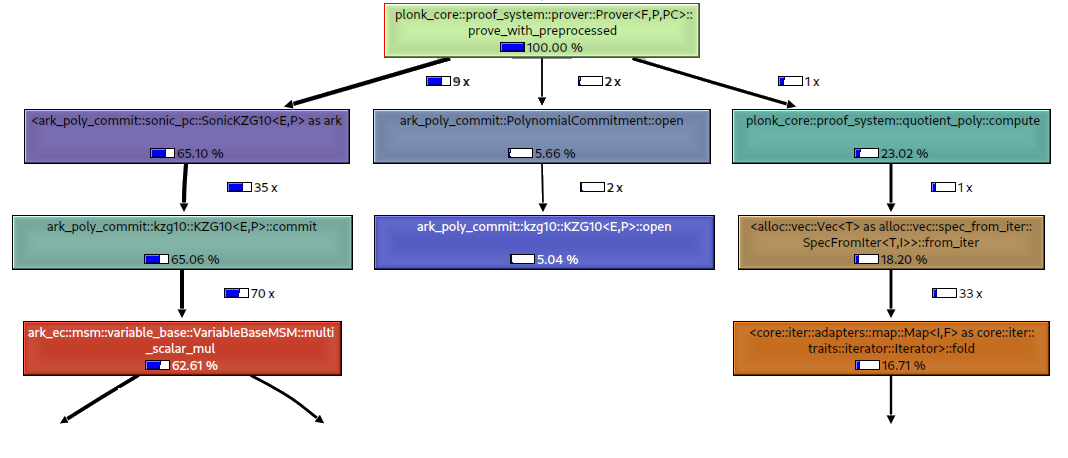
\includegraphics[width=1\linewidth]{figures//optimizations/computation_load.png}
    \caption{Computational Load of ZK-Garage implementation}
    \label{fig:profiler}
\end{figure}

Before trying out possible improvements, I analyzed demanding parts of the code. I used the popular profiling tool \textit{Callgrind} for that task. It monitors how often each function is called, along with the number of CPU instructions executed within each function. This allows for identifying the most computationally demanding function and prioritizing the efforts to ensure that the optimizations have the most significant impact on overall performance. 

The prover algorithm is contained in the function \texttt{prove\_with\_preprocessed}, which takes common preprocessed input as an argument. Figure \Cref{fig:profiler} shows the most demanding computation of the prover in a call graph. The most computationally heavy parts of the program are the computation of commitments and the construction of the quotient polynomial $t(x)$. From the computation of the prover algorithm, 65\% of the CPU instructions were spent on the commitments to the polynomials and 23\% on the construction of the quotient polynomial. The function that calculates the quotient polynomial is called only once, and there are two calls to polynomial openings at $\mathfrak{z}, \mathfrak{z}\omega$. As specified in the protocol, nine polynomial commitments correspond to the calls of the \texttt{commit} function. The profiler was executed on  $\textit{BenchCircuit}$ of size $2^{6}$, and the relative computation load varied depending on the circuit size. Nevertheless, most of the time is spent calculating commitments and the quotient polynomial $t(x)$, so optimizing it will be the goal for the rest of this chapter. Minimizing the number of commitments would mean the checks could be encoded more efficiently with fewer polynomial. This task is complex, but there are other ways to improve the performance. For example, it is possible to reduce the size of MSM in some of the commitments.

\section{Wire polynomials degree reduction}
In this work, I aimed to give a detailed explanation of the prover algorithm in the interactive protocol and decided to think of possible improvements in this area. I led a discussion on potential improvements with Tomáš Krňák \cite{tomas}, who suggested looking at the construction of wire polynomials $a(x), b(x), c(x)$, which are interpolated from the witness $\witness$. 

ZK-Garage interpolates $a(x), b(x), c(x)$ using inverse Fast Fourier transform ($\ifft$) implemented in \textit{arkworks}. The library calculates $\ifft$ using a variant of the Cooley–Tukey algorithm \cite{cooley-fft}, which requires the number of evaluations to be a power of two. The wire polynomial computed in round 1 also determines the degree of the polynomials computed in the following rounds. Reducing the degree of $ an (x), b(x), c(x)$ naturally speeds up the computation of $[a]_1, [b]_1, [c]_1$, but the construction and commitment of the quotient polynomial should also be faster. This makes it a meaningful candidate for optimization.

I have tried to reduce the degree of $a(x), b(x), c(x)$ in two ways suggested by Tomáš Krňák. It is possible to perform the reduction by polynomial division in coefficient form and also by pairwise division in evaluation form. The two approaches are sketched in the diagram \Cref{fig:degree-reduction}.

\subsection{Problem statement} 
The problem with the current implementation is that wire polynomials may be at most twice as big as the size of the circuit because of the padding to the next power of two. We denote the wire vector as $w = \{w_0, w_1 \ldots w_{m-1}\}$. The closest power of two to $m$ is $n$. To interpolate $w$ using $\ifft$, it needs to be padded to size $n$, which means that the size of SRS needs to be at least $n$. In the ZK-Garage, $w$ is padded with $n-m$ zeros. We denote the interpolated polynomial as: $$W(x) = w(x)pad_0(x)$$,
where $w(x)$ is defined by $w$ on the evaluation domain $H = \{1, \omega, \ldots \omega^{m-1}\}$ and $pad_0(x)$ is polynomial which has roots on $\{\omega^m, \omega^{m+1}, \omega^{n-1}\}$. We can write the padding polynomial as: 

\begin{equation}
    \label{padding-polynomail}
    pad_0(x) = (x - \omega^m)(x - \omega^m+1) \ldots (x - \omega^{n-1})
\end{equation}.

The reference implementation wire vector is padded and interpolated. There is no further degree reduction which means that $a(x), b(x), c(x)$ have degree $n-1$. It is also worth noting that the protocol does not perform any checks on the padding domain  $[\omega^{m}, \omega^{n-1}]$, which means we can pad the vectors with arbitrary values. As shown in the \Cref{chap:2}, the prover needs to show the following checks hold:

\begin{enumerate}
    \item Public input check: the public input is encoded in the first $l$ indices of the witness $\witness$, so values on $[\omega^{m}, \omega^{n-1}]$ do not concern it.
    \item Output check: the circuit output check verifies evaluation of the last element in the witness on $\omega^{m-1}$, therefore $[\omega^{m}, \omega^{n-1}]$ are not relevant for this case.
    \item Gate check: the values of the selectors $q_m(x), q_l(x), q_r(x), q_o(x), q_(x)$ on $[\omega^{m}, \omega^{n-1}]$ are zero because they do not encode any gate. Since $a(x), b(c), c(x)$ in the gate equation \Cref{gate-constraint} are always in combination with some selector the whole expression will evaluate to 0 as it should.
    \item Wiring check: the permutation function the the range $[\omega^{m}, \omega^{n-1}]$ encodes identity. This means that the wiring check does not enforce anything on $[\omega^{m}, \omega^{n-1}]$.
\end{enumerate}

Next, we present two optimizations that aim to use $\ifft$ to get $W(x)$ and reduce its degree to get $w(x)$. In the following sections, each approach will be described in detail.

\begin{figure}[H]
    \centering
    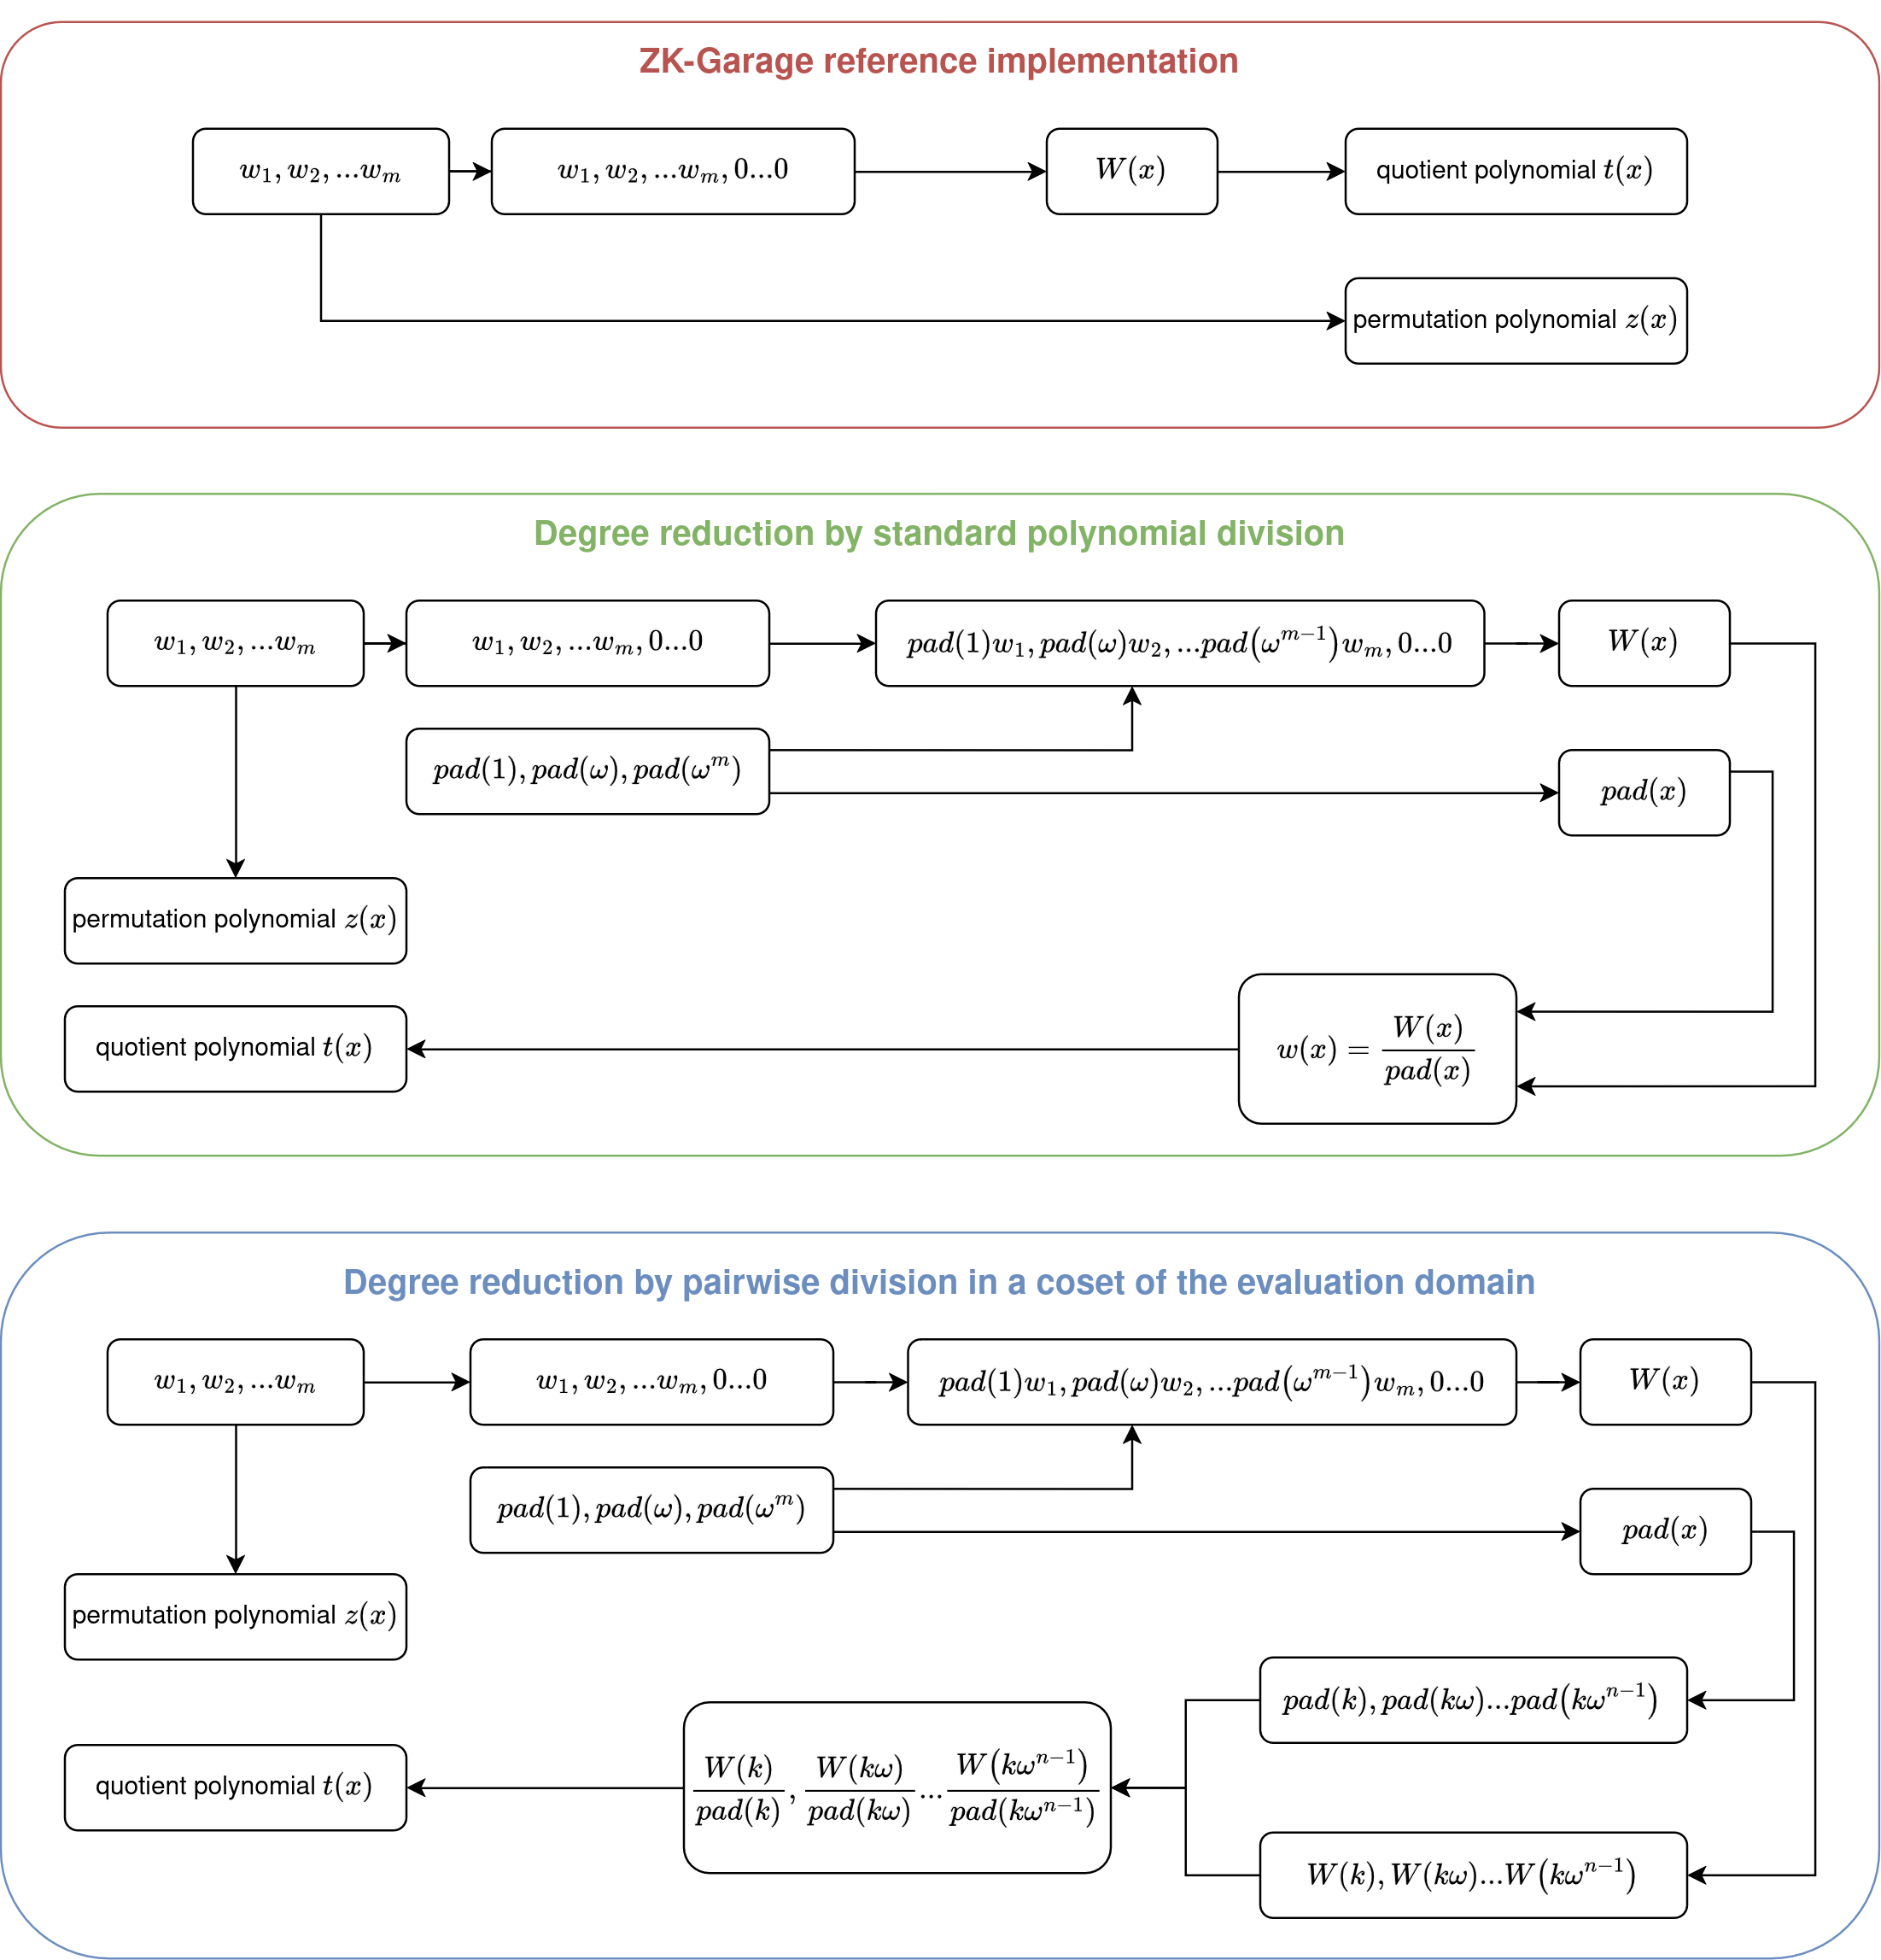
\includegraphics[width=1\linewidth]{figures/optimizations/degree_reduction_diagram.drawio.png}
    \caption{Degree reduction variants}
    \label{fig:degree-reduction}
\end{figure}

\subsection{ZK-Garage implementation}

\begin{pchstack}[center, boxed]
    \pseudocode[linenumbering, head=\textcolor{red}{Reference implementation in ZK-Garage}] {
        \text{construct padding vector } [0]^{n-m} \\
        \text{concatenate } [w, [0]^{n-m}] \\
        \text{interpolate } W(x) = \ifft(w, [0]^{n-m}) \\
        \pcreturn W(x)
    }
\end{pchstack}

The prover algorithm receives wire vectors $w_l, w_r, w_o$. These are padded with zeros and interpolated by $\ifft$ over the domain $H$ to get polynomial $a(x), b(x), c(x)$. Padded wire vectors are further used to calculate the permutation polynomial in \hyperref[chap:round2]{round 2} because, according to the protocol, the permutation polynomial is computed in the evaluation form.

\paragraph{Time analysis:} The complexity of this approach is dominated by $\ifft$, which has complexity $\bigO{n \log{n}}$.

\definecolor{ultramarine}{rgb}{0, 0.501, 0}
\subsection{Polynomial division}
\begin{pchstack}[center, boxed]
    \label{poly-div}
    \pseudocode[linenumbering, head=\textcolor{ultramarine}{Reduction by polynomial division}] {
        \text{construct padding vector } [0]^{n-m} \\
        \text{evaluate } [pad_0(1), pad_0(\omega), \ldots, pad_0(\omega^{m-1})] \\
        \text{concatenate } [w, [0]^{n-m}] \\
        \text{pair-wise multiplication } \Tilde{w} = [w_0 pad_0(1), \ldots w_{m-1} pad_0(\omega^{m-1}), 0 \ldots 0] \\
        \text{interpolate } W(x) = \ifft(\Tilde{w}) \\
        \text{reduce degree by polynomial division } w(x) = W(x) / pad_0(x) \\
        \pcreturn w(x)
    }
\end{pchstack}

The most straightforward approach when reducing the degree is to perform polynomial division by the polynomial defined by the padding values on $\{\omega^m, \ldots, \omega^{n-m}\}$. Note that $[w_0, w_1 \ldots w_{m}]$ first needs to be pair-wise multiplied by $[pad_0 \ldots pad_{m}]$ so that it holds $W(x) = w(x)pad(x)$. In this approach, I have used the standard algorithm for long polynomial division. As a result, it is possible to retrieve $w(x)$ of degree $m$ and use it in the following approach. The padded vector $[w_1, \ldots w_{m-1}, 0 \ldots 0]$ is again used in the round 2 to calculate $z(x)$. 

The zero padding polynomial could be written as $pad_0(x) = \prod_{i=m}^{n-1} (x - \omega^i)$. Computing values $[pad_0(1), pad_0(\omega) \ldots pad_0(\omega^{m-1})]$ requires significant number of field operations. There are $n-m$ field multiplications needed to calculate value $pad(\omega^i)$. To compute values on $[1 \ldots \omega^{m-1}]$, it is needed to perform $n-m \times m = nm - m^2$ field multiplication, which introduces non-negligible overhead. Luckily there is a better approach and evaluation of $pad_0(x)$ on $[1, \ldots \omega^m]$ can be calculated using recursive formula:
\begin{equation}
    \label{eq:recursive-formula}
    pad_0(x) =
    \begin{cases}
        \prod_{j=m}^{n-1} (1 - \omega^j) & x = 1,  \\
        \omega^{n-m-1} \frac{\omega^{i-1} - \omega^{m-1}}{\omega^{i-1} - \omega^{n-1}} pad_0(\omega^{i-1}) & x = \omega^i: i \in [m] \setminus \{1\}
    \end{cases}
\end{equation}

To confirm the correctness of this formula:
$$\frac{pad_0(\omega^i)}{pad_0(\omega^{i-1})} = \prod_{j = m}^{n-1} \frac{\omega^i - \omega^j}{\omega^{i-1} - \omega^j} = \omega^{n-m} \prod_{j = m}^{n-1} \frac{\omega^{i-1} - \omega^{j-1}}{\omega^{i-1} - \omega^j}$$
$$= \omega^{n-m} \frac{\omega(\omega^{i-1} - \omega^{m-1})}{\omega^{i-1} - \omega^{n-1}} = \omega^{n-m} \frac{\omega(\omega^{i-1} - \omega^{m-1})}{\omega^{i-1} - \omega^{n-1}}$$
$$pad_0(\omega^i) = \omega^{n-m} \frac{\omega(\omega^{i-1} - \omega^{m-1})}{\omega^{i-1} - \omega^{n-1}}pad_0(\omega^{i-1})$$


\paragraph{Time analysis:} Calculating evaluations of $pad$ can be done in $m$ iteration thanks to the recursive formula \Cref{eq:recursive-formula} and pairwise multiplication in step 4 of the algorithm could be trivially parallelized. Naive polynomial division, which has  complexity $deg(w(x))\times deg(pad_0(x)) = n \times n-m$, which makes the total complexity $n^2 - nm + n\log{n}$. Since $m < n/2$  we can conclude $\bigO{n^2 - \frac{3}{2}n}$.

From the analysis, we can already conclude that this approach will be much slower in round 1 than the former implementation. However it is questionable what is the performance benefit in rounds 2 - 5. As suggested by Tomáš Krňák \cite{tomas}, padding the circuit with a sparse polynomial might slightly speed up the polynomial division. One possibility is to use padding polynomial $pad_{cyclic}(x)$ that is zero on every $k$-th element of $H$ instead of  $pad_0(x)$ which is zero on $[\omega^m \ldots \omega^{n-1}]$, i.e.,

\begin{equation}
    pad_{cyclic}(x) = x^{\frac{n}{k}} - 1
\end{equation}.

The domain $H$ is generated by the $n$-th root of unity, so for every $\omega^ki$ it holds that:

$$pad_{cyclic}(\omega^{ki}) = \omega^{ki \frac{n}{k}} -1 = \omega^{ni} - 1 = 1^i - 1 = 0$$

This variant reduces the degree of the wire polynomial to $n - \frac{n}{k}$ instead of $m$. Moreover it requires changing the structure of the circuit. The witness $w_l, w_r, w_o$ selector $q_m, q_l, q_r, q_o, q_c$ and public input $PI$ need to be shifted in such way that every $k$-th index is 0, otherwise \Cref{eq:gate-contraints} fails. We also need to change the permutation function $\sigma^*$ accordingly. This would require a major change in the repository protocol. Therefore, I did not implement this alternative.

% , and we do not need to be contained to the $pad_{cyclic}(x)$.
As mentioned earlier, any value could be used as padding. We can try to find a different sparse polynomial to pad with. For example, we could pad by values of the polynomial that has a root at $\omega^m$ $pad_{m0}(x - \omega^m)$. However, this polynomial has only a degree 1, which means after the division, we get a reduction of degree by 1. This is not useful, so we have to state rough conditions for the polynomial we are searching for:

\begin{enumerate}
    \item polynomial is \textit{relatively} sparse
    \item has a \textit{high enough} degree
    \item is not zero on $[1, \omega^{m-1}]$
\end{enumerate}

Condition 1. should potentially achieve better performance in the polynomial division, and condition 2. should make sure that the division is worth it. One might ask if we could use a polynomial $x^{k}$ for padding. This polynomial is sparse, does not zero out on the domain $H$, and could have a sufficient degree. First, let us examine the case for $k=1$. If we divide a polynomial $W(x) = c_0 + c_1 x + c_2 + x^2 \ldots c_n x^n$ by $x$ we reduce the degree of each monomial as $c_0/x + c_1 + c_2 + x \ldots c_n x^{n-1}$. However, the problem is that $c_0$ is likely not divisible by $x$, which invalidates this approach. The same problem arises for larger $k$.

In the end, I did not succeed in finding a suitable polynomial. Even if such polynomial existed, it is unclear whether there is any reasonable performance gain. I have tried to measure naive polynomial division by polynomial $pad_0(x)$ and compare the time to other sparse polynomials on $n = 2^{14}$

\begin{table}[H]
    \centering
    \begin{tabular}{|l|l|l|l|l|}
    \hline
             & \multicolumn{1}{c|}{$pad_0$} & $x^{n/8}$ & $x^{n/4}$ & $x^{n/2}$ \\ \hline
    Time (s) & 152.1                        & 47.32     & 85.84     & 114.3     \\ \hline
    Degree   & 32766                        & 8192      & 163681    & 32768     \\ \hline
    \end{tabular}
\end{table}

Division by all of the sparse polynomials is faster than division by the zero-pad polynomial $pad_0(x)$. However, the efficiency mainly depends on the polynomial degree. In the case of this optimization, we would like to divide by a polynomial with a high degree to reduce the degree of the wire polynomial as much as possible. While division by $x^{n/4}$ is two times faster than division by $pad_0(x)$, this variant is still pretty slow, as seen in the \Cref{benchmarks}.

\subsection{Pairwise division}
\begin{pchstack}[center, boxed]
    \label{pairwise-div}
    \pseudocode[linenumbering, head=\textcolor{blue}{Reduction by pairwise division in domain coset}] {
        \text{construct padding vector } [0]^{n-m} \\
        \text{interpolate padding polynomial } pad_0 = \ifft([0]^{n-m}) \\
        \text{calculate coset evaluations } \cfft(pad_0(x)) = [pad_0(k1), \ldots, pad_0(k\omega^{m-1})] \\
        \text{concatenate } [w, [0]^{n-m}] \\
        \text{pair-wise multiplication } \Tilde{w} = [w_0 pad_0(1) \ldots w_{m-1} pad_0(\omega^{m-1}), 0 \ldots 0] \\
        \text{interpolate } W(x) = \ifft(\Tilde{w}) \\
        \text{calculate coset evaluations } \cfft(W(x)) = [W(k1) \ldots, W(k\omega^{m-1})] \\
        \text{reduce degree by pairwise division } \hat{w} = \left[\frac{W(k)}{pad_0(k)}, \frac{W(k\omega)}{pad_0(k\omega)} \ldots \frac{W(k\omega^{n})}{pad_0(k\omega^{n})}\right]  \\
        \text{interpolate } w(x) = \cifft(\hat{w}) \\
        \pcreturn w(x)
    }
\end{pchstack}

With the hope of bypassing the costs introduced by the polynomial division, we introduce the final approach, where the division is performed in the evaluation of the form. It is not possible to perform this computation on the domain $H$ because $pad_0(x)$ is zero on $[\omega^m \ldots \omega^{n-1}]$, which is why the division is performed in a coset of the domain $H$. As in the previous approach, both multiplication by the $pad_0(x)$ in $H$ and division by $pad_0(x)$ in the coset of $H$ could be trivially parallelized.

It might be a bit unclear why the reduction actually works since we interpolate $n$ values in step 6. We will not go into details about the $\fft$ algorithm, but we provide an intuition. The vector $w$ comes from a specific distribution determined by the circuit $\CRKT$, public input $\publicinput$, and the witness $\witness$, but we will assume that it is uniformly random. If we take $m$ evaluation of $w(x)$ and interpolate them over $H$, then with high probability, the evaluation on $[\omega^{m} \ldots \omega^{n}]$ would not be zero. To be more specific, for a uniformly random polynomial, the probability would be $\frac{1}{|\field|}^{n-m}$. This is why simply padding $w$ with zeros and using the $\ifft$ returns a polynomial $W(x)$ of degree $n-1$. However, if we instead divide by the evaluation of the padding polynomial in the coset of the evaluation domain, then all the $n$ evaluations correspond to the evaluations of $w(x)$, which has degree $m-1$. As a result, we get a polynomial of the degree $m-1$ from the interpolation.

Another trick that could make this approach faster is to precompute evaluations of $pad_0(x)$ on $H$ and the cost of $H$ in the protocol setup. The polynomial $pad_0(x)$ depends on $m$ which is determined by the size of $w$ and $deg(pad_0(x))$ could be anywhere in the interval $(\frac{n}{2}, n)$. The important thing is that $deg(pad(x)) \leq m$ because otherwise, the multiplication in step 5 of the algorithm would zero out part of $w$. So, we have to precompute evaluation for multiple sizes of $pad_0(x)$ and then use the suitable one. Although this approach does not completely reduce the degree to $m$, it is sufficient to gain performance benefits. In the implementation, we decided to precompute $\log{n/2}$ evaluation of $pad_0(x)$. This precomputation can save time when we are interested in a SNARK for the general circuit. However, when we want to run the prover only on a single circuit, we know the $m$ in advance and can precompute specific padding for $m$. 

\paragraph{Time analysis:} Evaluation of $pad_0(x)$ can be computed using the recursive formula \Cref{eq:recursive-formula}. However, this needs to be done only once in the protocol setup. Pairwise, multiplication, and division could be parallelized. The wire polynomial needs to be interpolated by $\ifft$, evaluated at coset by $\cfft$ and also interpolated on the coset using coset-$\ifft$. The total complexity is $3 n\log{n} = \bigO{n\log{n}}$.


\section{Benchmarks}
\label{benchmarks}

In the benchmarks, I compared two working implementations against the reference implementation. All measurements were taken on \textit{BenchCircuit}, which benchmarked ZK-Garage PlonK. The circuit contains only dummy constraints and can be constructed with a variable number of gates. To verify the correctness of my code, I ran it on other example circuits included in the repository. If the verifier accepts the proof produced, there is a good chance that the changes will not break the implementation. We provide a link to a \href{https://github.com/benbencik/plonk-polynomial-degree-reduction}{public repository} with the implemented optimization. 

\subsection{Local benchmarks}

% \begin{table}[]
% \begin{tabular}{|c|lll|lll|lll|}
% \hline
%  &
%   \multicolumn{3}{c|}{\textbf{Round 1}} &
%   \multicolumn{3}{c|}{\textbf{Round 2-5}} &
%   \multicolumn{3}{c|}{\textbf{Proving time}} \\ \hline
% \multicolumn{1}{|l|}{Circuit size} &
%   \multicolumn{1}{l|}{zkg} &
%   \multicolumn{1}{l|}{pw} &
%   poly &
%   \multicolumn{1}{l|}{zkg} &
%   \multicolumn{1}{l|}{pw} &
%   poly &
%   \multicolumn{1}{l|}{zkg} &
%   \multicolumn{1}{l|}{pw} &
%   poly \\ \hline
% $2^{8}$ &
%   \multicolumn{1}{l|}{0.004} &
%   \multicolumn{1}{l|}{0.016} &
%   0.019 &
%   \multicolumn{1}{l|}{0.317} &
%   \multicolumn{1}{l|}{0.367} &
%   0.311 &
%   \multicolumn{1}{l|}{0.321} &
%   \multicolumn{1}{l|}{0.385} &
%   0.330 \\ \hline
% $2^{10}$ &
%   \multicolumn{1}{l|}{0.006} &
%   \multicolumn{1}{l|}{0.063} &
%   0.159 &
%   \multicolumn{1}{l|}{0.800} &
%   \multicolumn{1}{l|}{0.962} &
%   0.803 &
%   \multicolumn{1}{l|}{0.806} &
%   \multicolumn{1}{l|}{1.026} &
%   0.963 \\ \hline
% $2^{12}$ &
%   \multicolumn{1}{l|}{0.029} &
%   \multicolumn{1}{l|}{0.088} &
%   1.923 &
%   \multicolumn{1}{l|}{2.943} &
%   \multicolumn{1}{l|}{2.656} &
%   2.621 &
%   \multicolumn{1}{l|}{2.972} &
%   \multicolumn{1}{l|}{2.744} &
%   4.544 \\ \hline
% $2^{14}$ &
%   \multicolumn{1}{l|}{0.032} &
%   \multicolumn{1}{l|}{0.260} &
%   30.67 &
%   \multicolumn{1}{l|}{9.441} &
%   \multicolumn{1}{l|}{8.784} &
%   9.393 &
%   \multicolumn{1}{l|}{9.473} &
%   \multicolumn{1}{l|}{9.045} &
%   40.06 \\ \hline
% \end{tabular}
% \end{table}

\begin{figure}
    \centering
    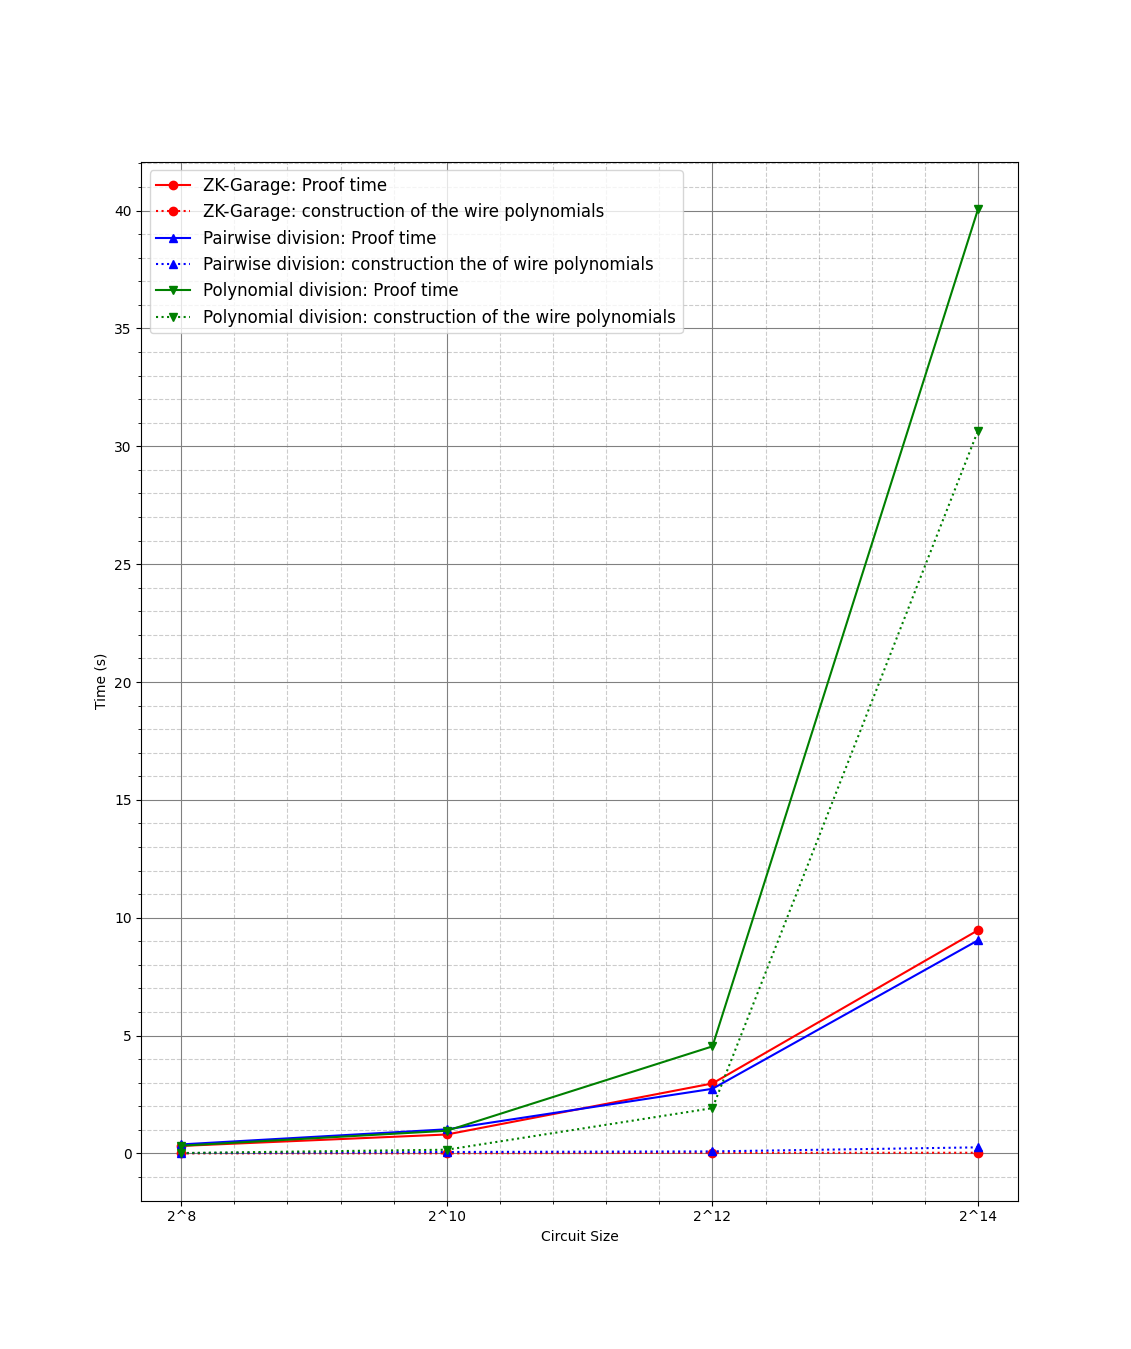
\includegraphics[width=1\linewidth]{figures/optimizations/local_bench.png}
    \caption{Local benchmarks on AMD Ryzen 7 5800H}
    \label{fig:local-bench}
\end{figure}

I compared the two implementations from \Cref{poly-div} and \Cref{pairwise-div} against the reference implementation. At first, I ran the benchmarks locally on a consumer-grade notebook. The major limitation was the memory capacity due to the size of SRS. I measured the total proving time and the time needed to construct the wire polynomials. The plot in \Cref{fig:local-bench} shows that the version with a naive polynomial division is unsurprisingly much worse than the ZK-Garage implementation. Construction of the wire polynomials alone takes 3 times the construction of the proof in ZK-Garage. Therefore, I will not consider this approach in further benchmarks. 

The alternative with pairwise division \Cref{pairwise-div} introduces overhead in the construction of the wire polynomials because it introduces additional $\fft$s. The improvement raises with the size of the circuit, which follows from the fact that the increased size of the circuit leads to greater padding. And the bigger the padding is, the more we can reduce the degree of the wire polynomials, resulting in improvements in rounds 2-5. So, for circuits of bigger size, the performance benefit becomes more pronounced. However, the improvement is much lower than what we were hoping for. To get insight into the problem, I measured what was happening in rounds 2-5. 

\subsection{Remote benchmarks}
The rest of the measurements were taken on servers of the Department of Applied Mathematics of the Faculty of Mathematics and Physics of Charles University. The machine has CPU type \textit{Intel Xeon E5-2630 v3} with 16 cores and frequency 3200 MHz. The memory usage after the setup of the protocol for the circuit of size $2^{20}$ reached 50GB, and the whole protocol filled the entire memory of 125GB on the circuit of size $2^{21}$. In addition to the proving time and the construction of wire polynomial $a(x), b(x), c(x)$, I have measured also commitments to these polynomials $[a]_1, [b]_1, [c]_1$ and also commitments to the quotient polynomial that is split into multiple parts as described in the round 3. Table \ref{table-measurements} shows the exact comparison between the reference implementation and the degree reduction described by pairwise division in the coset \ref{pairwise-div} in seconds. These results are as well plotted on \Cref{fig:kam-bench}.

\label{table-measurements}
\begin{table}[H]
    \centering
    \begin{tabular}{|l|llll|llll|}
    \hline
     &
      \multicolumn{4}{c|}{ZK-Garage} &
      \multicolumn{4}{c|}{Reduced Degree} \\ \hline
    \multicolumn{1}{|l|}{\begin{tabular}[c]{@{}l@{}}Circuit\\ size\end{tabular}} & 
      \multicolumn{1}{l|}{\begin{tabular}[c]{@{}l@{}}$a(x)$\\ $b(x)$\\ $c(x)$\end{tabular}} &
      \multicolumn{1}{l|}{\begin{tabular}[c]{@{}l@{}}$[a]_1$\\ $[b]_1$\\ $[c]_1$\end{tabular}} &
      \multicolumn{1}{l|}{$[t]_1$} &
    \multicolumn{1}{l|}{\begin{tabular}[c]{@{}l@{}}Proof\\ time\end{tabular}} & 
      \multicolumn{1}{l|}{\begin{tabular}[c]{@{}l@{}}$a(x)$\\ $b(x)$\\ $c(x)$\end{tabular}} &
      \multicolumn{1}{l|}{\begin{tabular}[c]{@{}l@{}}$[a]_1$\\ $[b]_1$\\ $[c]_1$\end{tabular}} &
      \multicolumn{1}{l|}{$[t]_1$} &
   \multicolumn{1}{l|}{\begin{tabular}[c]{@{}l@{}}Proof\\ time\end{tabular}} \\ \hline
    $2^{15}$ &
      \multicolumn{1}{l|}{0.023} &
      \multicolumn{1}{l|}{0.413} &
      \multicolumn{1}{l|}{0.466} &
      7.393 &
      \multicolumn{1}{l|}{0.102} &
      \multicolumn{1}{l|}{0.260} &
      \multicolumn{1}{l|}{0.467} &
      7.000 \\ \hline
    $2^{16}$ &
      \multicolumn{1}{l|}{0.039} &
      \multicolumn{1}{l|}{0.834} &
      \multicolumn{1}{l|}{0.856} &
      14.325 &
      \multicolumn{1}{l|}{0.183} &
      \multicolumn{1}{l|}{0.491} &
      \multicolumn{1}{l|}{0.883} &
      13.882 \\ \hline
    $2^{17}$ &
      \multicolumn{1}{l|}{0.061} &
      \multicolumn{1}{l|}{1.499} &
      \multicolumn{1}{l|}{1.487} &
      27.369 &
      \multicolumn{1}{l|}{0.341} &
      \multicolumn{1}{l|}{0.843} &
      \multicolumn{1}{l|}{1.489} &
      26.035 \\ \hline
    $2^{18}$ &
      \multicolumn{1}{l|}{0.133} &
      \multicolumn{1}{l|}{2.894} &
      \multicolumn{1}{l|}{2.954} &
      54.144 &
      \multicolumn{1}{l|}{0.692} &
      \multicolumn{1}{l|}{1.642} &
      \multicolumn{1}{l|}{2.972} &
      52.479 \\ \hline
    $2^{19}$ &
      \multicolumn{1}{l|}{0.244} &
      \multicolumn{1}{l|}{5.393} &
      \multicolumn{1}{l|}{5.110} &
      106.628 &
      \multicolumn{1}{l|}{1.268} &
      \multicolumn{1}{l|}{3.182} &
      \multicolumn{1}{l|}{5.310} &
      103.123 \\ \hline
    $2^{20}$ &
      \multicolumn{1}{l|}{0.499} &
      \multicolumn{1}{l|}{9.166} &
      \multicolumn{1}{l|}{9.166} &
      201.599 &
      \multicolumn{1}{l|}{2.615} &
      \multicolumn{1}{l|}{5.555} &
      \multicolumn{1}{l|}{10.817} &
      198.667 \\ \hline
    \end{tabular}
\end{table}

\begin{figure}
    \centering
    \label{fig:kam-bench}
    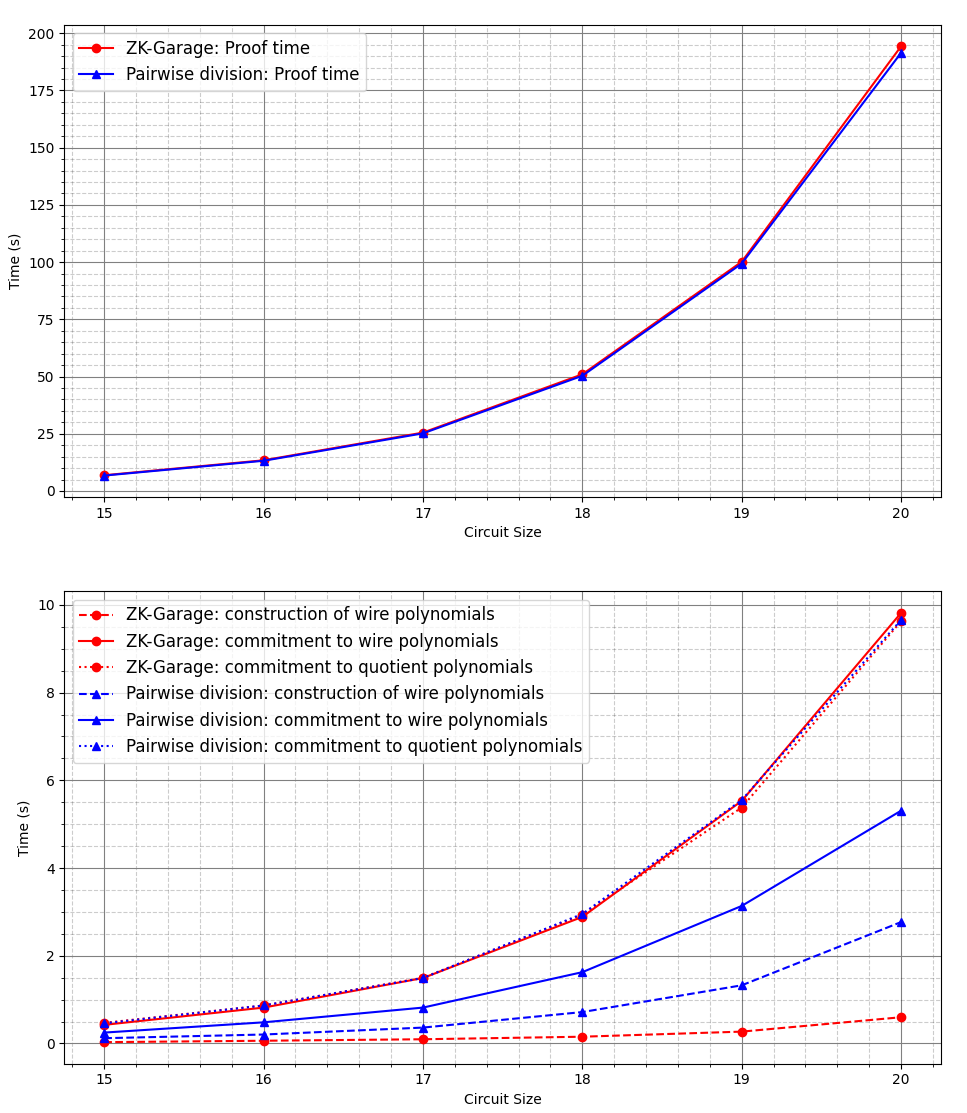
\includegraphics[width=1\linewidth]{figures/optimizations/kam_bench.png}
    \caption{Remote benchmarks on Intel Xeon E5-2630 v3}
\end{figure}

It is again evident that the improvement in the proof time is negligible. Time for the commitment of the wire polynomial decreased significantly as it should; however, the commitment of the quotient polynomial did not change at all. In this optimization, we wanted to reduce the degree of the wire polynomial with the hope the polynomial $t(x)$ constructed from the wire polynomials would also have a smaller degree. Since commitments to the quotient polynomial take approximately the same time and the complexity of commitment is dominated MSM, it must mean that the degree of the quotient polynomial $t(x)$ does not change at all. 

Going back to the ZK-Garage implementation, I found out that the quotient polynomial is computed in the evaluation form, unlike the protocol description in the original paper \cite{plonk}. First, all of the required polynomials are transformed into a coset of the domain $H$ of size 8n. This is due to a similar reason as in \Cref{pairwise-div} to avoid division by 0. Each of the parts of the quotient polynomial is computed in the evaluation form. Finally, they are merged and interpolated through coset-$\ifft$. The resulting polynomial is split into 8 parts, and the prover calculates the commitment to each of them. The reason why the polynomial needs to be split into 8 parts is that the \Cref{eq:gate-contraints} is extended with checks for custom gates, and there is also an additional polynomial proving the validity of the lookup table. As a result, the degree of $t(x)$ is determined by interpolation, and the reduction of the wire polynomial does not affect the degree of the quotient polynomial. 

\begin{pchstack}[center, boxed]
    \pseudocode[linenumbering, head=ZK-Garage Round 3] {
        \text{evaluate polynomial on coset of domain of size } 8n \\
        \text{calculate } t_1(x) \ref{quotient1}, t_2(x) \ref{quotient2} t_3(x) \ref{quotient3} \text{ in the evaluation form} \\
        \text{calculate polynomial } t_4(x) \text{ for proving correctness of the lookup table } \\
        \text{merge and interpolate } t(x) = \cifft(t_1(x) + t_2(x) + t_3(x) + t_4(x)) \\ 
        \text{split the result into 8 polynomials and calculate corresponding commitments }
    }
\end{pchstack}

We can conclude that the only performance benefit of the optimization \ref{pairwise-div} is in the computation of commitments $[a]_1, [b]_1, [c]_1$ and the quotient polynomial is computed from evaluations of wire polynomials. We know that it is possible to compute the commitment form a polynomial in evaluation form as explained in \Cref{sec:kzg-evaluation-form}, so if it even needed to construct the polynomials $a(x), b(x), c(x)$? Round 3 uses the evaluation wire polynomials in the cost of the domain, which is easy to compute. The problem is that there are $8n$ evaluations instead of $n$. We have described how to compute a new evaluation with precomputed barycentric weights in $n$ operation. That means calculating the evaluations on the domain of size 8n will take $8n^2$, which is slow. However, if there is a smarter way to do this that is comparable to $n \log{n}$, we could skip the computation of $ a(x), b(x), c(x)$ together. 

In conclusion, the optimization with degree reduction of the wire polynomials did not bring the desired performance benefit for this implementation of the $\plonk$ protocol due to the reason that round 3 is computed in another way than in the description of the protocol. 

\subsection{Engineering approach}
Designing a more efficient variant of the $\plonk$ protocol is undoubtedly a hard task, and sometimes, an engineering approach might produce good results. Even though this was not the purpose of the work, there are many possible improvements on the software side. The most notable difference was produced by parallelized computations in round 2 and round 3. As already discussed, the construction of the wire protocol takes a significant portion of the proving time, which becomes even more pronounced for circuits of larger size. Since the quotient polynomial is computed in the evaluation form, the whole computation is trivially parallelizable. We improved the function for computing $t(x)$ by a parallelized approach to computing the evaluation of the polynomial for gate constraints, permutation constraints, and lookup table constraints. A similar approach also helped to speed up the construction of the permutation polynomial $z(x)$ in round 2. This approach was implemented using the parallel iterator in \href{https://github.com/rayon-rs/rayon}{rayon}, which is a lightweight data parallelism library that guarantees data race freedom. In the next measurement, we compared the approach \Cref{pairwise-div} with parallel computation of $t(x)$ and $z(x)$. As can be seen from the results \Cref{fig:parallelized}, this change yields a significantly faster prover algorithm. 

\begin{table}[H]
\scriptsize
\begin{tabular}{|l|lll|lll|lll|}
\hline
 &
  \multicolumn{3}{c|}{permutaiton polynomial} &
  \multicolumn{3}{c|}{quotient polynomial} &
  \multicolumn{3}{c|}{total proof time} \\ \hline
Degree &
  \multicolumn{1}{l|}{zkg.} &
  \multicolumn{1}{l|}{par.} &
  imp. &
  \multicolumn{1}{l|}{zkg.} &
  \multicolumn{1}{l|}{par.} &
  imp. &
  \multicolumn{1}{l|}{zkg.} &
  \multicolumn{1}{l|}{par.} &
  imp. \\ \hline
$2^{15}$ &
  \multicolumn{1}{l|}{0.23} &
  \multicolumn{1}{l|}{0.05} &
  76.52\% &
  \multicolumn{1}{l|}{3.72} &
  \multicolumn{1}{l|}{1.41} &
  62.13\% &
  \multicolumn{1}{l|}{6.84} &
  \multicolumn{1}{l|}{4.18} &
  38.88\% \\ \hline
$2^{16}$ &
  \multicolumn{1}{l|}{0.46} &
  \multicolumn{1}{l|}{0.10} &
  77.73\% &
  \multicolumn{1}{l|}{7.40} &
  \multicolumn{1}{l|}{2.77} &
  62.58\% &
  \multicolumn{1}{l|}{13.39} &
  \multicolumn{1}{l|}{8.13} &
  39.28\% \\ \hline
$2^{17}$ &
  \multicolumn{1}{l|}{0.89} &
  \multicolumn{1}{l|}{0.18} &
  79.42\% &
  \multicolumn{1}{l|}{14.72} &
  \multicolumn{1}{l|}{5.56} &
  62.25\% &
  \multicolumn{1}{l|}{25.55} &
  \multicolumn{1}{l|}{15.16} &
  40.66\% \\ \hline
$2^{18}$ &
  \multicolumn{1}{l|}{1.80} &
  \multicolumn{1}{l|}{0.33} &
  81.58\% &
  \multicolumn{1}{l|}{29.56} &
  \multicolumn{1}{l|}{11.64} &
  60.63\% &
  \multicolumn{1}{l|}{51.02} &
  \multicolumn{1}{l|}{30.48} &
  40.26\% \\ \hline
$2^{19}$ &
  \multicolumn{1}{l|}{3.55} &
  \multicolumn{1}{l|}{0.66} &
  81.44\% &
  \multicolumn{1}{l|}{59.56} &
  \multicolumn{1}{l|}{23.24} &
  60.99\% &
  \multicolumn{1}{l|}{100.75} &
  \multicolumn{1}{l|}{59.26} &
  41.18\% \\ \hline
$2^{20}$ &
  \multicolumn{1}{l|}{7.11} &
  \multicolumn{1}{l|}{1.37} &
  80.71\% &
  \multicolumn{1}{l|}{120.17} &
  \multicolumn{1}{l|}{47.00} &
  60.89\% &
  \multicolumn{1}{l|}{195.09} &
  \multicolumn{1}{l|}{112.38} &
  42.40\% \\ \hline
\end{tabular}
\end{table}

While we have mentioned other design optimizations of the protocol, it might be also meaningful to work on an engineering solution. There have already been multiple attempts for hardware optimization of computationally expensive tasks like MSM, one of which is covered in the paper \cite{pipeMSM}.


\begin{figure}
    \centering
    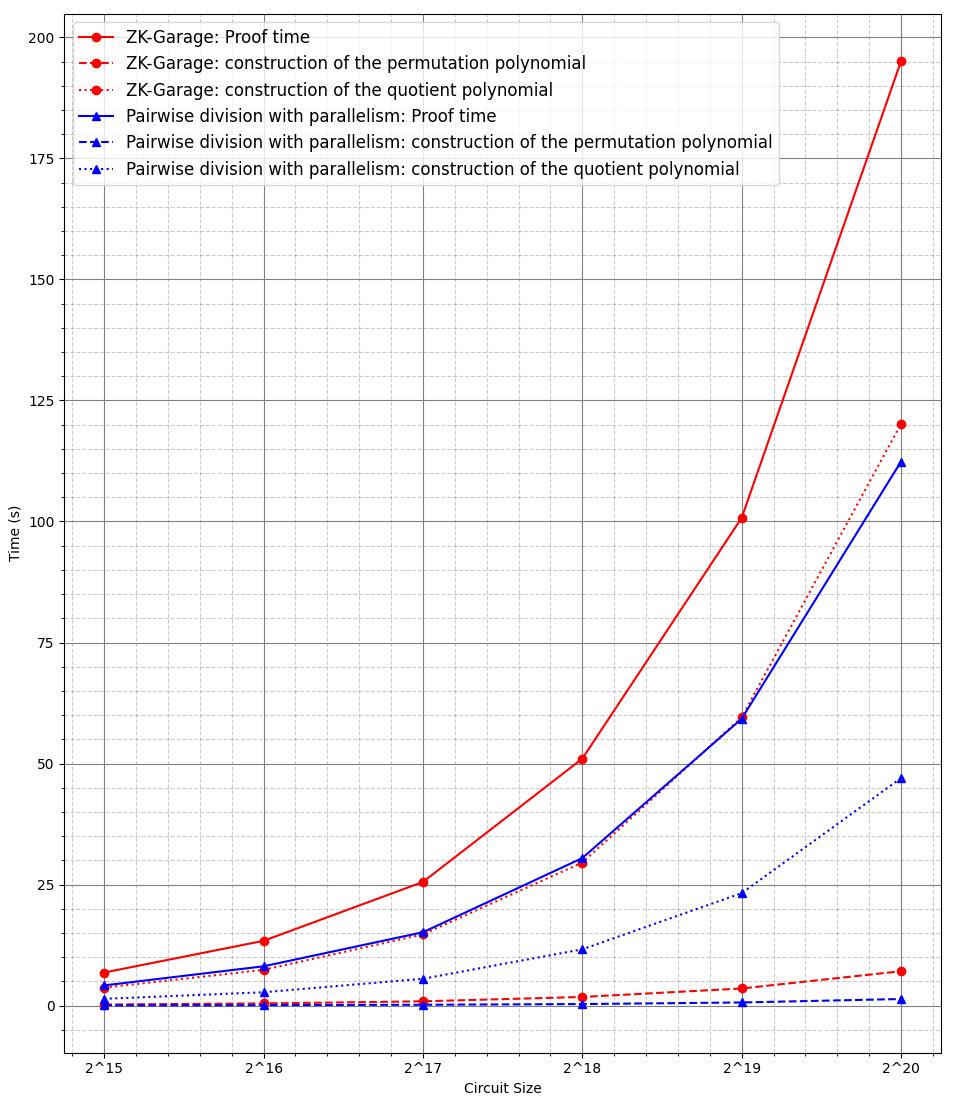
\includegraphics[width=1\linewidth]{figures//optimizations/parallel.png}
    \caption{Parallel computation of the quotient polynomial}
    \label{fig:parallelized}
\end{figure}


\hl{TODO}
\begin{itemize}
    \item Still do not understand the PKoE assumption
    \item Establish complexity of elliptic curve arithmetic
    \item Choose specific pairing.
    \item Which form of curve representation is used? (Weierstrass, Montgomery, Twisted-Edwards)
    \item Lagrange basis polynomial -> commitments can be evaluated from the evaluation form great explanation at scroll
\end{itemize}

%%% References 
%%% References are sought in the database priklady_literatury.bib.
%%% Requires the compilation sequence latex->bibtex->latex->latex
\bibliography{references}

%%% List of figures
\listoffigures

%%% List of tables
\listoftables

%%% 
%\chapter*{List of abbreviations}
%\addcontentsline{toc}{chapter}{List of abbreviations}


%%% The Appendix. 
%\chapter*{Appendix}
%\addcontentsline{toc}{chapter}{Appendix}



\end{document}

